\documentclass{cmspaper}
\usepackage{color}
\usepackage{graphicx}
\usepackage{wrapfig}
\usepackage{slashbox}
\usepackage{epstopdf}  %added for MAC compiler
\usepackage{pdfpages}
\usepackage{lineno}
\usepackage{verbatim}
\usepackage{url}
\RequirePackage{lineno} 
%\RequirePackage{lineno} 

\usepackage{wrapfig}

%Note to authors: these definitions are suggested to be used for consistency
\newcommand{\pt}{$p_T$ }
\newcommand{\GeVc}{GeV/c}
\newcommand{\mll}{\ensuremath{M_{\ell\ell}}}
\newcommand{\z}{$Z$ }
\newcommand{\zjets}{$\rm{Z}+\rm{jets}$ }
\newcommand{\gjets}{$\gamma+\rm{jets}$ }
\newcommand{\Z}{$Z$ } %redundancy can be good
\newcommand{\ttbar}{\ensuremath{t\bar{t}}}
\newcommand{\ttV}{\ensuremath{t\bar{t}\rm{V}}}
\newcommand{\emu }{\ensuremath{e\mu}}
\newcommand{\ee  }{\ensuremath{ee}}
\newcommand{\eepm}{\ensuremath{e^+ e^-}}
\newcommand{\mm  }{\ensuremath{\mu\mu}}
\newcommand{\mmpm}{\ensuremath{\mu^+ \mu^-}}
\newcommand{\empm}{\ensuremath{e^\pm \mu^\mp}}
\newcommand{\ase}[2]{\ensuremath{_{~- #1}^{~+ #2}}}
\newcommand{\MET}{\ensuremath{\rm{E_{T}^{miss}}}}
\newcommand{\met}{\mbox{$\raisebox{.3ex}{$\not$}E_T$\hspace*{0.5ex}}} 
\newcommand{\effr}{$R_{e\mu}$} %used to be \epsilon
\newcommand{\effrm}{$R_{\mu e}$} %used to be \epsilon
\newcommand{\sta}{$\sigma\times A$} %notation is such that A includes BR
\newcommand{\statistics}{CL$_\mathrm{S}$}
\newcommand{\njets}{$N_{\rm{jets}}$}
%\newcommand{\chizi}{\ensuremath{\widetilde{\chi}^{0}_{1}}\xspace}
%\newcommand{\chipm}{\ensuremath{\widetilde{\chi}^{\pm}_{1}}\xspace}
%\newcommand{\chizii}{\ensuremath{\widetilde{\chi}^{0}_{2}}\xspace}

\newcommand{\chizi}{\ensuremath{\tilde{\chi}^{0}_{1}}}
\newcommand{\chipm}{\ensuremath{\tilde{\chi}^{\pm}_{1}}}
\newcommand{\chizii}{\ensuremath{\tilde{\chi}^{0}_{2}}}

%The lumi so that if it changes it's easier to update
\newcommand{\lumi}{19.5~fb$^{-1}$}

%loose(tight) signal region met cut
\newcommand{\signalmetl}{100}
\newcommand{\signalmett}{200}
\newcommand{\signalmetvt}{300}

\newcommand{\resulttitle}
%{                       &   MET $>30$  GeV    &   MET $>60$  GeV    &   MET $>100$ GeV    &   MET $>200$ GeV \\}
%{                       &   MET $>30$  GeV    &   MET $>60$  GeV    &   MET $>100$ GeV    &   MET $>200$ GeV  &  MET $>300$ GeV  \\}
%move 300 to 150
{                       &   MET $>30$  GeV    &   MET $>60$  GeV    &   MET $>100$ GeV    &   MET $>150$ GeV  &  MET $>200$ GeV  \\}

\newcommand{\wjets}{$\rm{W}+{\rm jets}$}
\newcommand{\zzmet}{$\rm{ZZ}+\MET$}
\newcommand{\wzmet}{$\rm{WZ}+\MET$}
\newcommand{\wzzmet}{$\rm{WZ/ZZ}+\MET$}
\newcommand{\Ht}{$H_{T}$}
\newcommand{\cls}  {\ensuremath{\mathrm{CL_S}}}


\begin{document}


%\begin{comment}

\begin{titlepage}

  %\internalnote{2011/000}
  \cmsnote{2011/254}

  \date{\today}
 
  \title{Searches for beyond-the-standard model physics in events with a Z boson, jets and missing transverse energy}

  %No Victor this time (sorry, Victor)
  \begin{Authlist}
    D.~Barge, C.~Campagnari, D.~Kovalskyi, V.~Krutelyov
    \Instfoot{ucsb}{University of California, Santa Barbara, USA}

    W.~Andrews, G.~Cerati, D.~Evans, F.~Golf, I.~MacNeill, S.~Padhi, V.~Welke, Y.~Tu, F.~W\"urthwein, 
	A.~Yagil, J.~Yoo
    \Instfoot{ucsd}{University of California, San Diego, USA}

	L.~Bauerdick, K.~Burkett, I.~Fisk, Y.~Gao, O.~Gutsche, B.~Hooberman, S.~Jindariani, J.~Linacre, V.~Martinez Outschoorn
    \Instfoot{fnal}{Fermi National Accelerator Laboratory, Batavia, Illinois, USA}
  \end{Authlist}

  \begin{abstract}

This note describes a search for beyond-the-standard model (BSM) physics in events with a leptonically-decaying Z boson, 
jets, and missing transverse energy (\MET).
This signature is predicted to occur in several BSM scenarios, for example supersymmetric (SUSY) models.
Two search strategies are pursued. The first is an inclusive approach which selects events with at least two jets and
large \MET, produced in association with the Z$\to\ell\ell$ candidate. The second is a targeted search 
in which additional requirements are imposed in order to achieve sensitivity to the production of the weakly-coupled
SUSY charginos and neutralinos. The main backgrounds of SM \zjets\ and \ttbar\ production are estimated with the data-driven 
\MET\ templates technique and the opposite-flavor subtraction technique, respectively.
Additional backgrounds are estimated from simulation, after validation in data control samples. 
In both the inclusive and targeted analyses,  good agreement is observed between the data and predicted background over the full \MET\ range. 
The results are interpreted in the context of a simplified SUSY model, and used to place constraints on the masses of the electroweak
charginos and neutralinos.

\end{abstract}

\end{titlepage}

%\end{comment}

\setcounter{page}{2}%JPP


\newpage
\tableofcontents

\newpage
\linenumbers
\section{Changes w.r.t. previous AN Version}
\label{sec:changes}

\begin{itemize}

\item v6: Updated to full 2012 sample corresponding to 19.3 fb$^{-1}$.
\item v5: {\bf This is the version corresponding to the HCP results}. Added interpretation for the GMSB model (Sec.~\ref{sec:interpretation}). Added data vs. MC kinematic distributions for the sample with 3 leptons and at least 2 jets, where we observe an excess of data with respect to the MC prediction (App.~\ref{app:WZ}).
\item v4: Un-blinded the results of the inclusive and targeted analysis, and added an interpretation in the \wzmet\ model. Moved the material for the edge analysis to a separate AN (2012/359).
\item v3: Added results for the low-\MET\ and high-\MET\ signal regions used for the edge analysis, for the first 5.1 fb$^{-1}$ 2012A+B data.
\item v2: Updated to 9.2 fb$^{-1}$ of 53X data and MC (v1 used 5.1 fb$^{-1}$ 52X data and MC).

\end{itemize}

\section{Introduction}
\label{sec:intro}

In this note we describe a search for new physics in the 2011 
opposite sign isolated dilepton sample ($ee$, $e\mu$, and $\mu\mu$).  
The main source of 
isolated dileptons at CMS is Drell Yan and $t\bar{t}$.
Here we concentrate on dileptons with invariant mass inconsistent
with $Z \to ee$ and $Z \to \mu\mu$.  Thus $t\bar{t}$ is the most
important background.  A separate search for new physics in the $Z$ 
sample is described in a separate note\cite{ref:Ztemplates}.
This is an update of an analysis performed on 2010 data~\cite{ref:osnote,ref:ospaper}. 

The search strategy is the following

\begin{itemize}

\item We start out with a pre-selection which is as close as 
possible to the published (or soon to be published) $t\bar{t}$
dilepton analysis\cite{ref:top} (same lepton ID, same jet definitions,
etc.).  We do make a couple of substantive modifications:

\begin{enumerate}
\item The top analysis requires two leptons of $P_T > 20$ GeV.  
 In this
analysis we lower the requirement on the second lepton to $P_T > 10$ 
GeV.  This is motivated by our desire to maintain sensitivity to possible
SUSY signals with relatively low $P_T$ leptons generated in the 
cascade decays of heavy objects.
\item The top analysis requires at least two jets of $P_T > 30$
GeV with \met $>30$ GeV ($ee$ and $e\mu$) or \met $>20$ GeV ($e \mu$).
We tighten the \met cut to 50 GeV and we 
also require that the scalar sum of the $P_T$ of all jets with $P_T > 30$
GeV be $> 100$ GeV.  These requirements considerably
reduce backgrounds to the $t\bar{t}$ sample, {\em e.g.}, backgrounds
from Drell Yan and $W+$jets.
\end{enumerate}

\item The pre-selection consists mostly of $t\bar{t}$ events.  We perform 
data $-$ Monte Carlo comparisons of kinematical distributions.  Assuming
reasonable agreeement for the bulk of $t\bar{t}$ we move on to a 
search for new physics in the tail of the $t\bar{t}$.

\item Our prejudice is that new physics would manifest itself in an
excess of events with high \met and significant hadronic activity.
We define an a-priori search region by tightening the \met and 
hadronic activity requirements such that we expect of order 1\% 
of $t\bar{t}$ events to pass the selection (as predicted by Monte Carlo).

\item We perform a counting experiment in the signal region.  We compare
observed yields with expectations from Monte Carlo and with two independent
data driven techniques (see Section~\ref{sec:abcd} and~\ref{sec:victory}).

\end{itemize}





\section{Datasets}
\label{sec:datasets}

%\subsection{Datasets}

%We use a combination of rereco and prompt reco for both leptons and photons.
We use the May 10 ReReco and prompt reco data for both signal and control samples.%leptons and photons.
\\
For selecting the dilepton sample, the following datasets are used (the pythia DY samples are used only for generator level Z mass values less than 50 to avoid overlap with the madgraph DYJets sample), including the benchmark SUSY points LM4 and LM8:


\begin{itemize}
\item Data 
\begin{itemize}
\item \verb=/DoubleElectron/Run2011A-May10ReReco-v1/AOD=
\item \verb=/DoubleMu/Run2011A-May10ReReco-v1/AOD=
\item \verb=/MuEG/Run2011A-May10ReReco-v1/AOD=

\item \verb=/DoubleElectron/Run2011A-PromptReco-v4/AOD=
\item \verb=/DoubleMu/Run2011A-PromptReco-v4/AOD=
\item \verb=/MuEG/Run2011A-PromptReco-v4/AOD=
\end{itemize}

\item Monte Carlo
  \begin{itemize} 
  \item \verb=/DYJetsToLL_TuneD6T_M-50_7TeV-madgraph-tauola/Spring11-PU_S1_START311_V1G1-v1/AODSIM=
  \item \verb=/TTJets_TuneZ2_7TeV-madgraph-tauola/Spring11-PU_S1_START311_V1G1-v1/AODSIM=
  \item \verb=/WJetsToLNu_TuneZ2_7TeV-madgraph-tauola/Spring11-PU_S1_START311_V1G1-v1/AODSIM=
  \item \verb=/WWTo2L2Nu_TuneZ2_7TeV-pythia6/Spring11-PU_S1_START311_V1G1-v1/AODSIM=
  \item \verb=/WZtoAnything_TuneZ2_7TeV-pythia6-tauola/Spring11-PU_S1_START311_V1G1-v1/AODSIM=
  \item \verb=/ZZtoAnything_TuneZ2_7TeV-pythia6-tauola/Spring11-PU_S1_START311_V1G1-v1/AODSIM=
  \item \verb=/TToBLNu_TuneZ2_s-channel_7TeV-madgraph/Spring11-PU_S1_START311_V1G1-v1/AODSIM=
  \item \verb=/TToBLNu_TuneZ2_t-channel_7TeV-madgraph/Spring11-PU_S1_START311_V1G1-v1/AODSIM=
  \item \verb=/TToBLNu_TuneZ2_tW-channel_7TeV-madgraph/Spring11-PU_S1_START311_V1G1-v1/AODSIM=
  \item Pythia samples:
  \item \verb=/DYToEE_M-20_CT10_TuneZ2_7TeV-powheg-pythia/Spring11-PU_S1_START311_V1G1-v1/AODSIM=
  \item \verb=/DYToMuMu_M-20_CT10_TuneZ2_7TeV-powheg-pythia/Spring11-PU_S1_START311_V1G1-v1/AODSIM=
  \item \verb=/DYToTauTau_M-20_CT10_TuneZ2_7TeV-powheg-pythia-tauola/Spring11-PU_S1_START311_V1G1-v1/AODSIM=
  \item \verb=/DYToEE_M-10To20_TuneZ2_7TeV-pythia6/Spring11-PU_S1_START311_V1G1-v1/AODSIM=
  \item \verb=/DYToMuMu_M-10To20_TuneZ2_7TeV-pythia6/Spring11-PU_S1_START311_V1G1-v1/AODSIM=
  \item LM samples:
  \item \verb=/LM4_SUSY_sftsht_7TeV-pythia6/Spring11-PU_S1_START311_V1G1-v1/AODSIM=
  \item \verb=/LM8_SUSY_sftsht_7TeV-pythia6/Spring11-PU_S1_START311_V1G1-v1/AODSIM=
  \end{itemize}
\end{itemize}

For the creation of photon templates, we use:

\begin{itemize}
\item \verb=/Photon/Run2011A-May10ReReco-v1/AOD=
\item \verb=/Photon/Run2011A-PromptReco-v4/AOD=
%\item \verb==
\end{itemize}

The integrated luminosity used corresponds to \lumi, and the JSON used is 
the official May 10 ReReco 
and July 1 prompt reco
JSON:
\\
Cert\_160404-163869\_7TeV\_May10ReReco\_Collisions11\_JSON.txt
%Cert_160404-163869_7TeV_May10ReReco_Collisions11_JSON.txt
\\
Cert\_160404-167784\_7TeV\_PromptReco\_Collisions11\_JSON.txt
%Cert_160404-167784_7TeV_PromptReco_Collisions11_JSON.txt

%\clearpage


\section{Studies of Jets from Pileup}
\label{sec:pujets}

In order to ensure the jets which pass the jet selection are from the hard collision rather than from pileup (PU), we will use MC truth information to define a method in which we can distinguish between these jets.

The following dataset is used:

\begin{itemize}
\scriptsize
\item \verb=/DYJetsToLL_M-50_TuneZ2Star_8TeV-madgraph-tarball/Summer12_DR53X-PU_S10_START53_V7A-v1/AODSIM=
\end{itemize}

\subsection{Selection}
The preselection requirements from the inclusive analysis are used to study the PU jets, specifically:

\begin{itemize}
\item Require two leptons which both pass the lepton selection with \pt $>$ 20 \GeVc 
\item 81 GeV $<$ \mll $<$ 101 GeV
\item Require at least two jets both with \pt $> 30$ \GeVc~and $|\eta| < 2.5$ 
\end{itemize}

\subsection{Defining Jets to be ``Matched'' to Genjets}
In order to determine which jets are from the hard collision and which jets come from PU using the MC truth information, the $\Delta$R between each pfjet and the closest status 1 generator level jet with \pt $>$ 20 \GeVc is calculated. By examining the distribution in Fig. \ref{fig:dralljets} we choose a cut value of $\Delta$R $<$ 0.4 to define our jets as ``matched'' to a genjet, and if $Delta$R $>$ 0.4, then the jet is defined to be a PU jet.

%% dr of all jets plot
\begin{figure}[!h]
\begin{center}
\begin{tabular}{cc}
%% 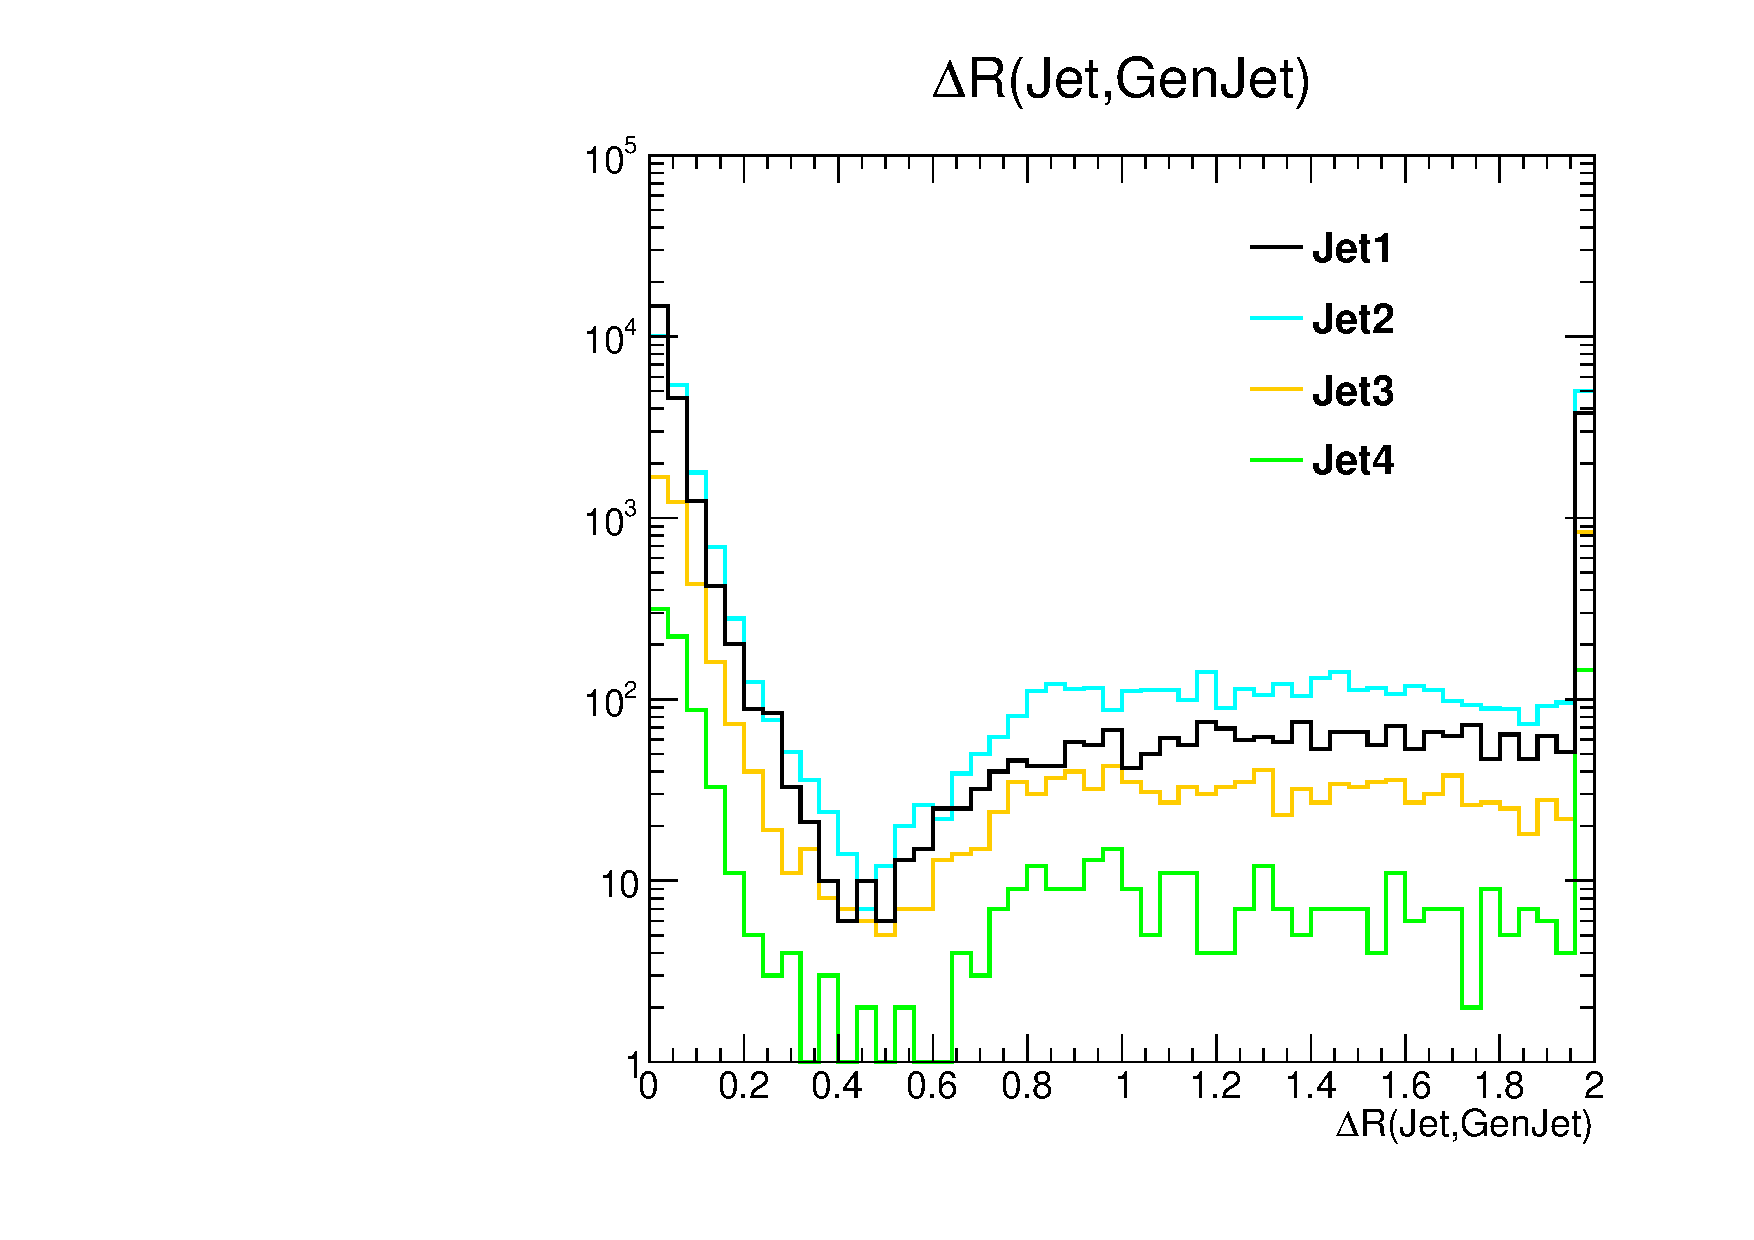
\includegraphics[width=0.6\textwidth]{/home/users/cwelke/public_html/Zmet/jetstudy/pdf/jetAlldrgen_Inclusive_Selection.pdf}
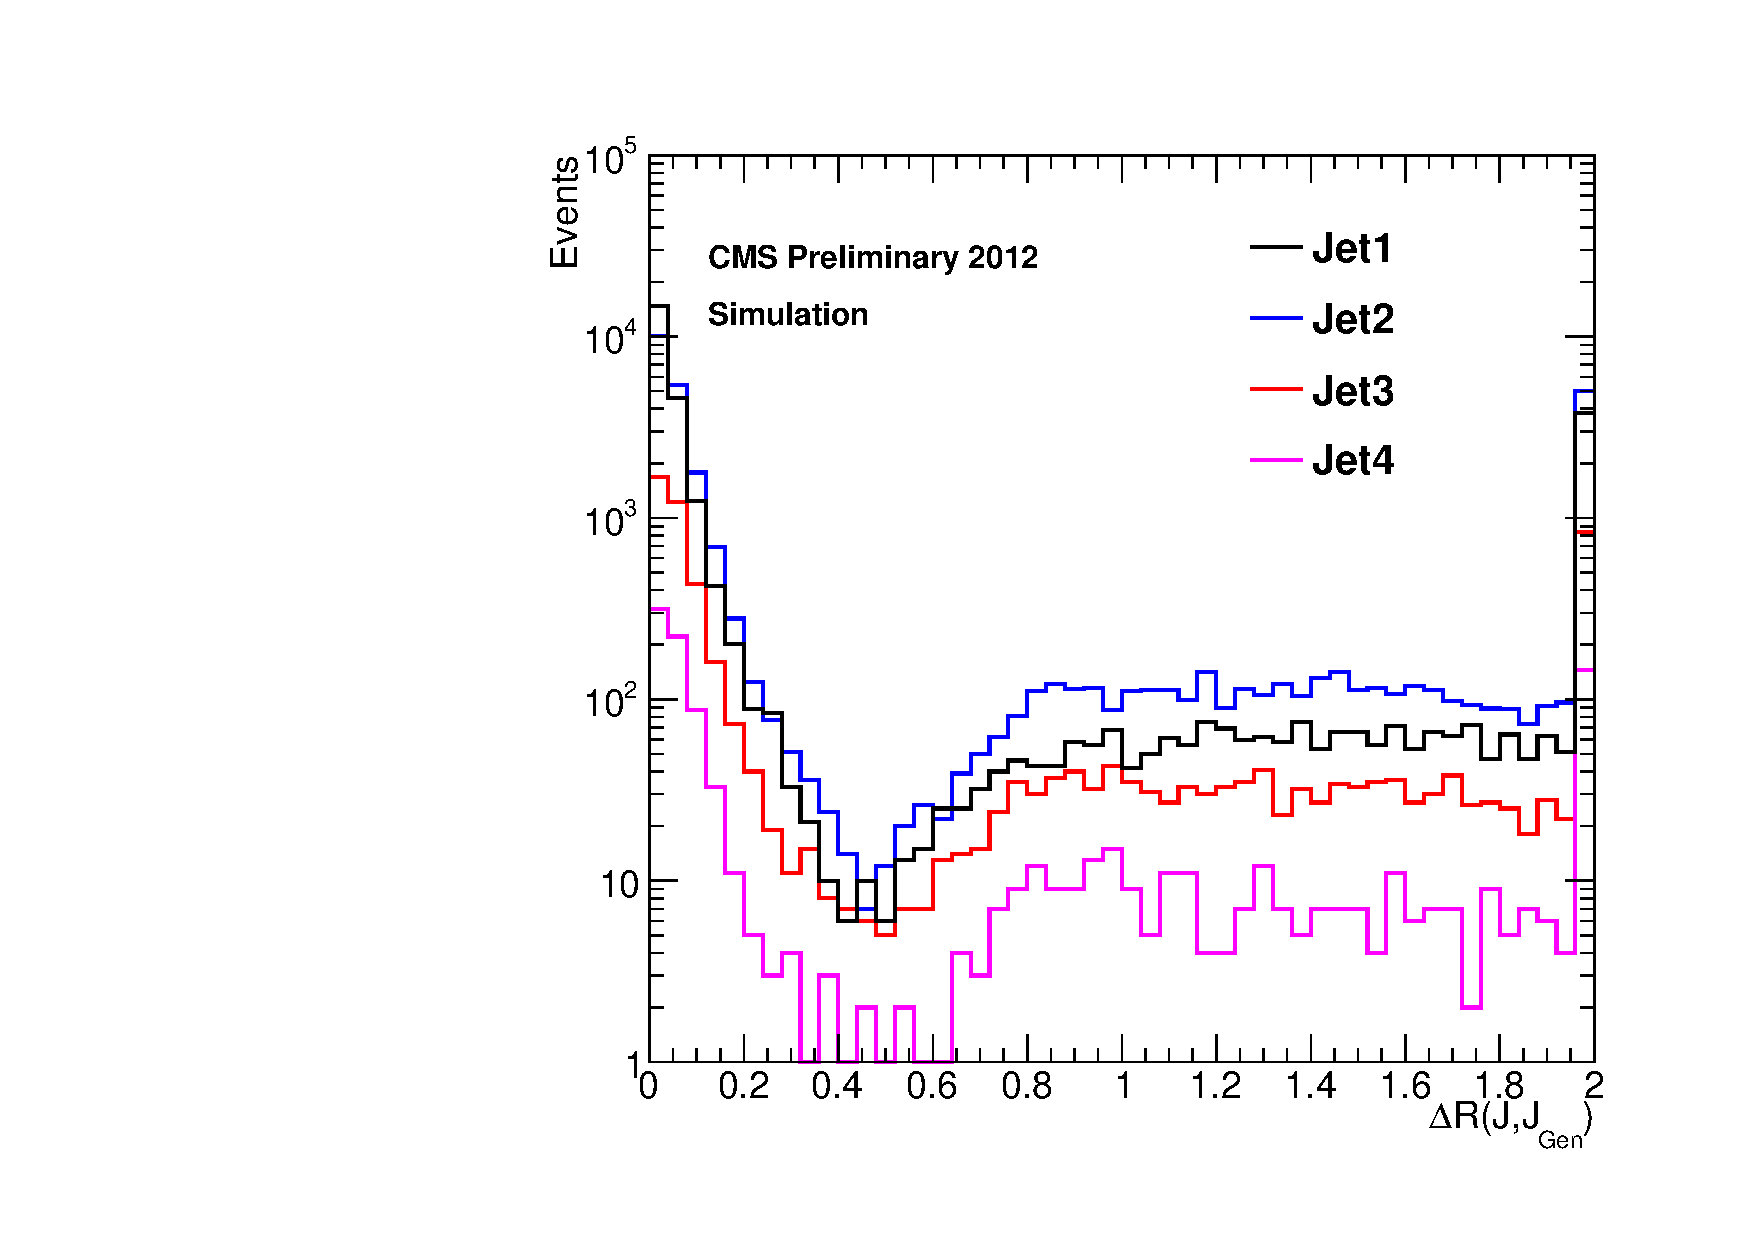
\includegraphics[width=0.6\textwidth]{plots/dralljets.pdf}
\end{tabular}
\caption{The $\Delta$R for the four highest \pt jets is shown. We are using $\Delta$R $<$ 0.4 to define jets to be ``matched'' to a genjet.
\label{fig:dralljets}
}
\end{center}
\end{figure}

\subsection{Defining $\beta$}
Now that we've established how to distinguish between PU jets versus hard scatter jets using MC truth information, we want to be able to be able to make the same distinction in data (without the truth information). In order to do this, the variable $\beta$ is defined for each jet in equation (\ref{eqn:beta}) 

\begin{equation}
\beta = \frac{\sum_i({track~p_T^i})^2_{tracks~with~dz~>~0.5~cm}}{\sum_i ({track~p_T^i})^2_{All~Tracks}}
\label{eqn:beta}
\end{equation}

Jets with $\beta$ close to 1 are jets from the hard collision, whereas Jets with $\beta$ close to 0 are PU jets. By looking at the $\beta$ distribution of the two highest \pt jets in Figure.~\ref{fig:jetbeta}, we choose a cut value of $\beta$ $>$ 0.2 to remove PU jets. 

%% The plots in Fig.~\ref{fig:jetbeta} show the $\beta$ distributions for the two highest \pt jets after being seperated as PU jets and hard scatter jets.

%% jet beta plots
\begin{figure}[!hbtp]
\centering
\subfigure[]{
\centering
\label{subfig:jet1beta}
%% \includegraphics[width=.4\textwidth]{/home/users/cwelke/public_html/Zmet/jetstudy/pdf/jet1beta2_05.pdf}
\includegraphics[width=.4\textwidth]{plots/jet1beta2_05.pdf}
}
\subfigure[]{
\centering
\label{subfig:jet2beta}
%% \includegraphics[width=.4\textwidth]{/home/users/cwelke/public_html/Zmet/jetstudy/pdf/jet2beta2_05.pdf}
\includegraphics[width=.4\textwidth]{plots/jet2beta2_05.pdf}
}\\
\caption{$\beta$ for jet1 \subref{subfig:jet1beta} and jet2 \subref{subfig:jet2beta}.}
\label{fig:jetbeta}
\end{figure}

We list the efficiencies for the $\beta$ cut in table \ref{table:efficiency}

\begin{table}[htb]
\begin{center}
\caption{\label{table:efficiency} Selection efficiencies for a cut value of $\beta > 0.2$. }
\begin{tabular}{l|cc}
\hline
\hline
$\beta > 0.2$ & PU Jets & Hard Scatter Jets \\
\hline
Jet 1 & 12\% & 99\% \\
Jet 2 & 17\% & 99\% \\
\hline
\hline
\end{tabular}
\end{center}
\end{table}

\subsection{Dilepton \pt}
These plots show the dilepton mass of events which pass the inclusive analysis selection. As you can see in Fig.~\ref{fig:dileppt}, the PU jets have a significant contribution to the shape of the distribution at low \pt. The rejection of PU jets leads to a dilepton \pt distribution which looks healthy (i.e. the double peak structure is gone). 

%% dilepton Pt Plots
\begin{figure}[!hbtp]
\centering
\subfigure[]{
\centering
\label{subfig:jet1cut}
%% \includegraphics[width=.4\textwidth]{/home/users/cwelke/public_html/Zmet/jetstudy/pdf/dilep_Pt_jet1_drgen_Selection.pdf}
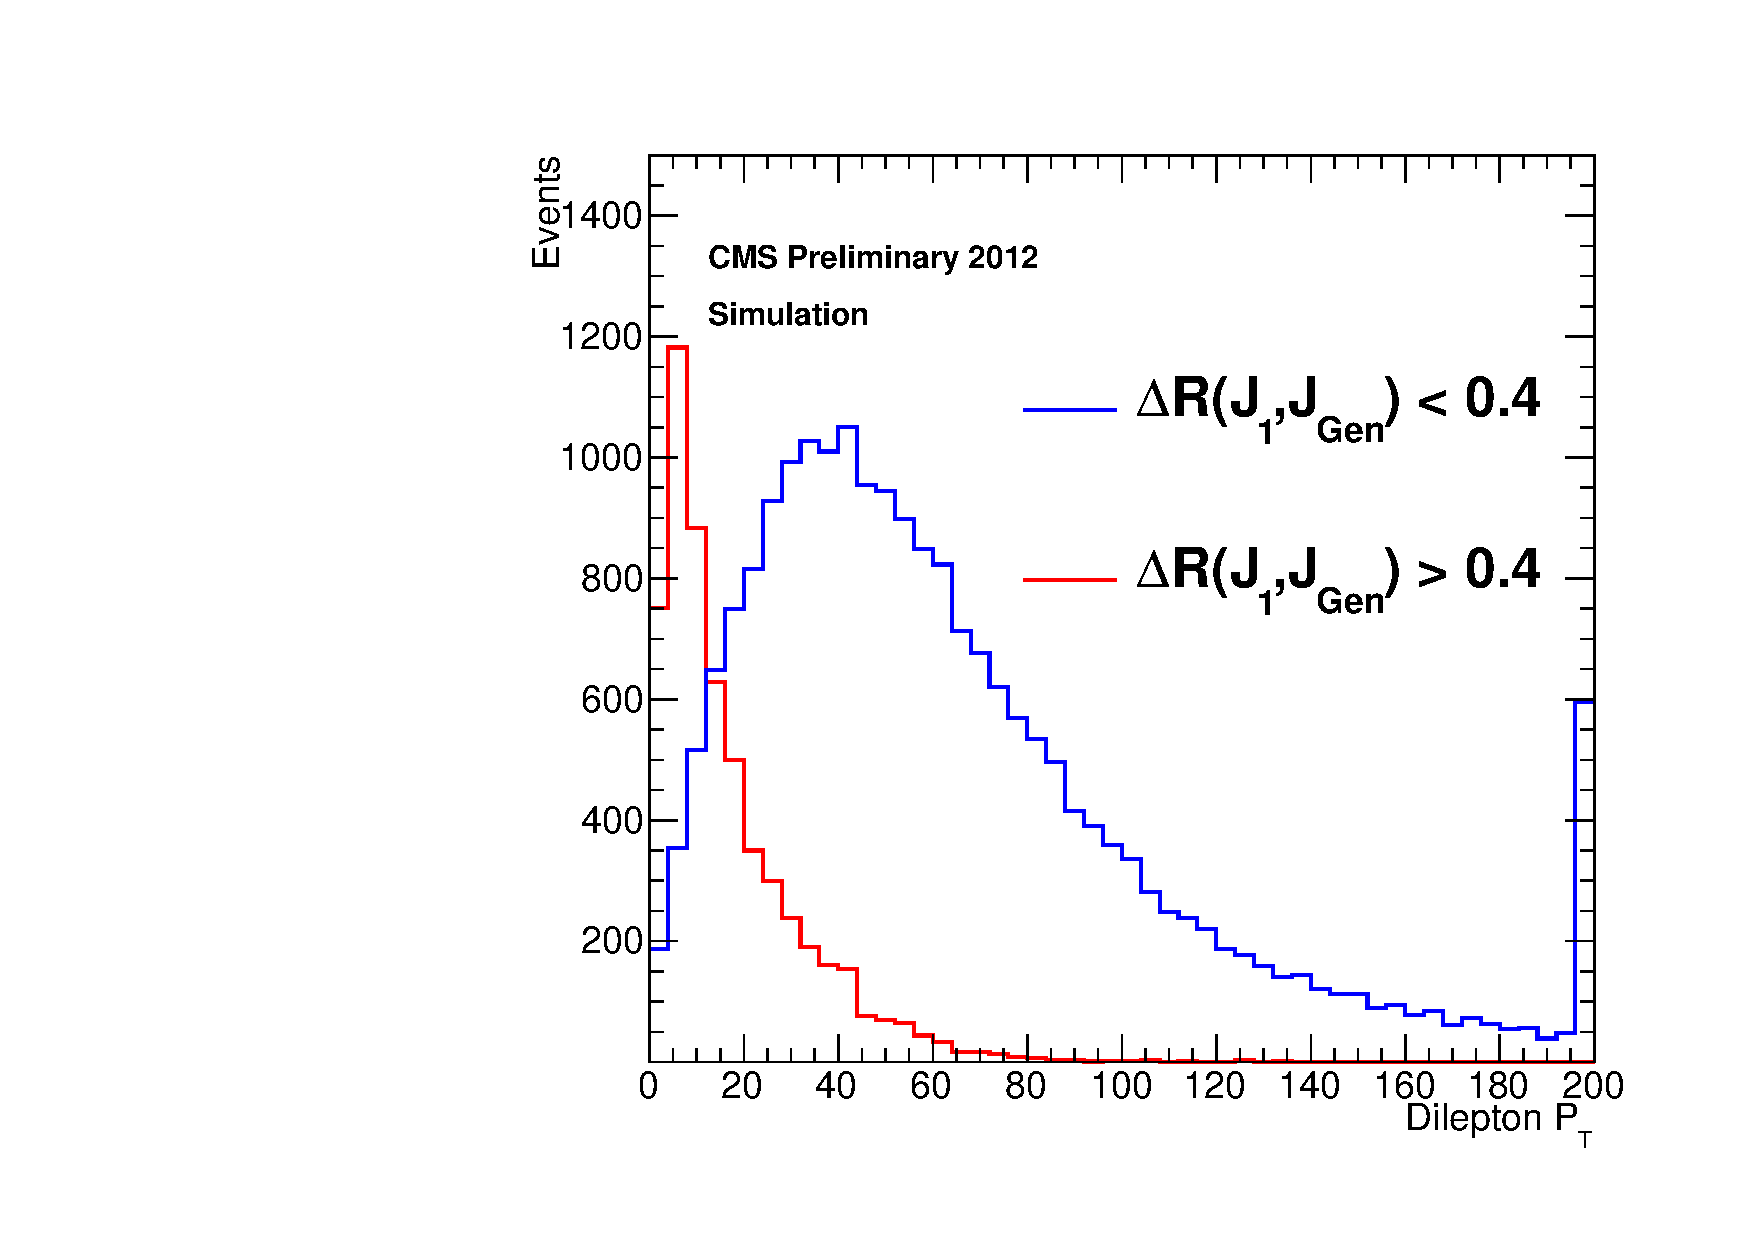
\includegraphics[width=.4\textwidth]{plots/dilep_pt_jet1.pdf}
}
\subfigure[]{
\centering
\label{subfig:jet12cut}
%% \includegraphics[width=.4\textwidth]{/home/users/cwelke/public_html/Zmet/jetstudy/pdf/dilep_Pt_jet1_jet2_drgen_Selection.pdf}
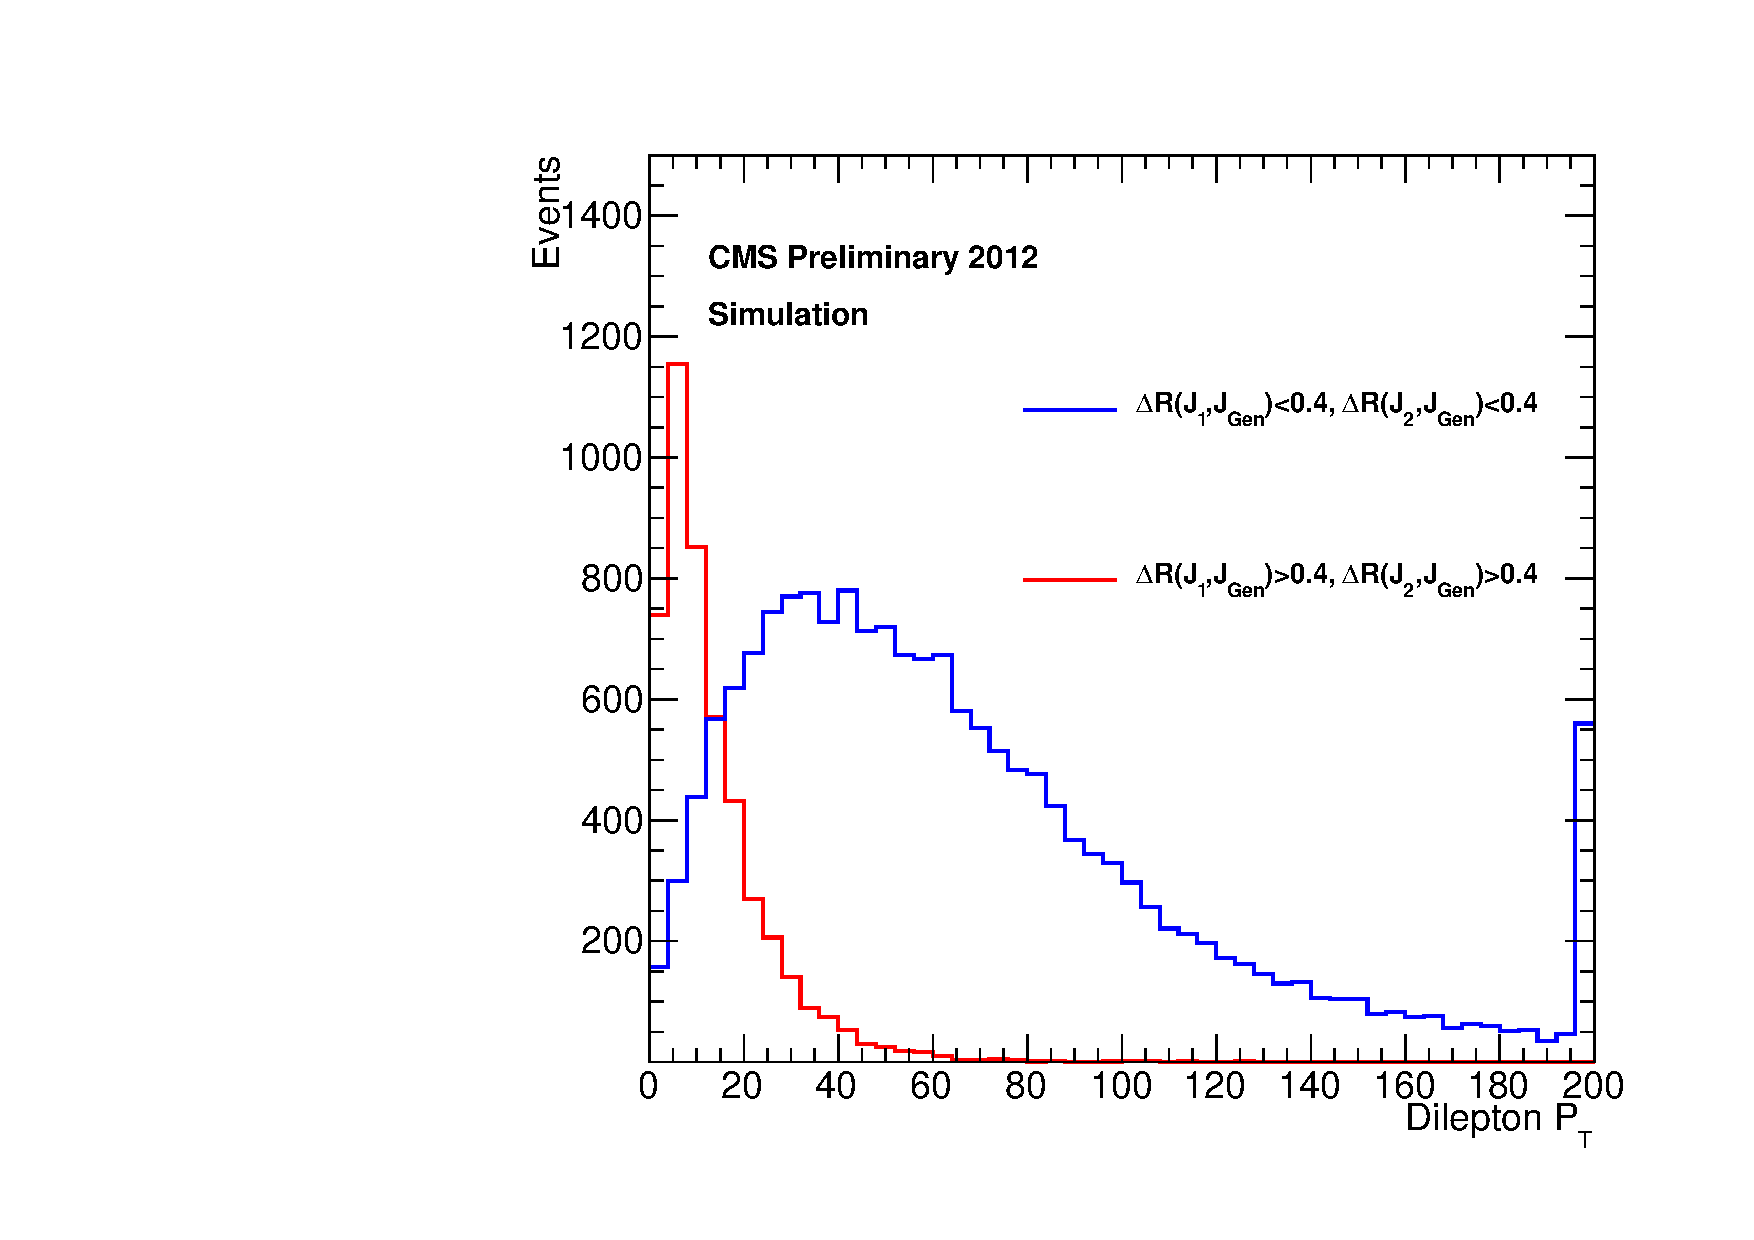
\includegraphics[width=.4\textwidth]{plots/dilep_pt_jet1_jet2.pdf}
}\\
\caption{Dilepton \pt with $\Delta$R cut on jet1 \subref{subfig:jet1cut} and $\Delta$R cut on jet1 and jet2 \subref{subfig:jet12cut}.}
\label{fig:dileppt}
\end{figure}


\subsection{Distinguishing Event Type}
If we seperate the jets in the event by jet type (i.e. PU jets vs hard scatter jets), we can determine what type of event we are looking at. The possible event types are \z + 2 hard scatter jets, \z + 1 hard scatter jet and 1 PU jet, and \z + 2 PU jets. 
In Fig.~\ref{fig:2Ddrplot}, the $\Delta$R between the highest \pt jet and its associated gen jet is plotted against the $\Delta$R between the second highest \pt jet and its associated gen jet. We can use this plot to visually see the various regions which contain the three different event types.

%% dr of all jets plot
\begin{figure}[!h]
\begin{center}
\begin{tabular}{cc}
%% \includegraphics[width=0.6\textwidth]{/home/users/cwelke/public_html/Zmet/jetstudy/pdf/2D_drgen_Selection.pdf}
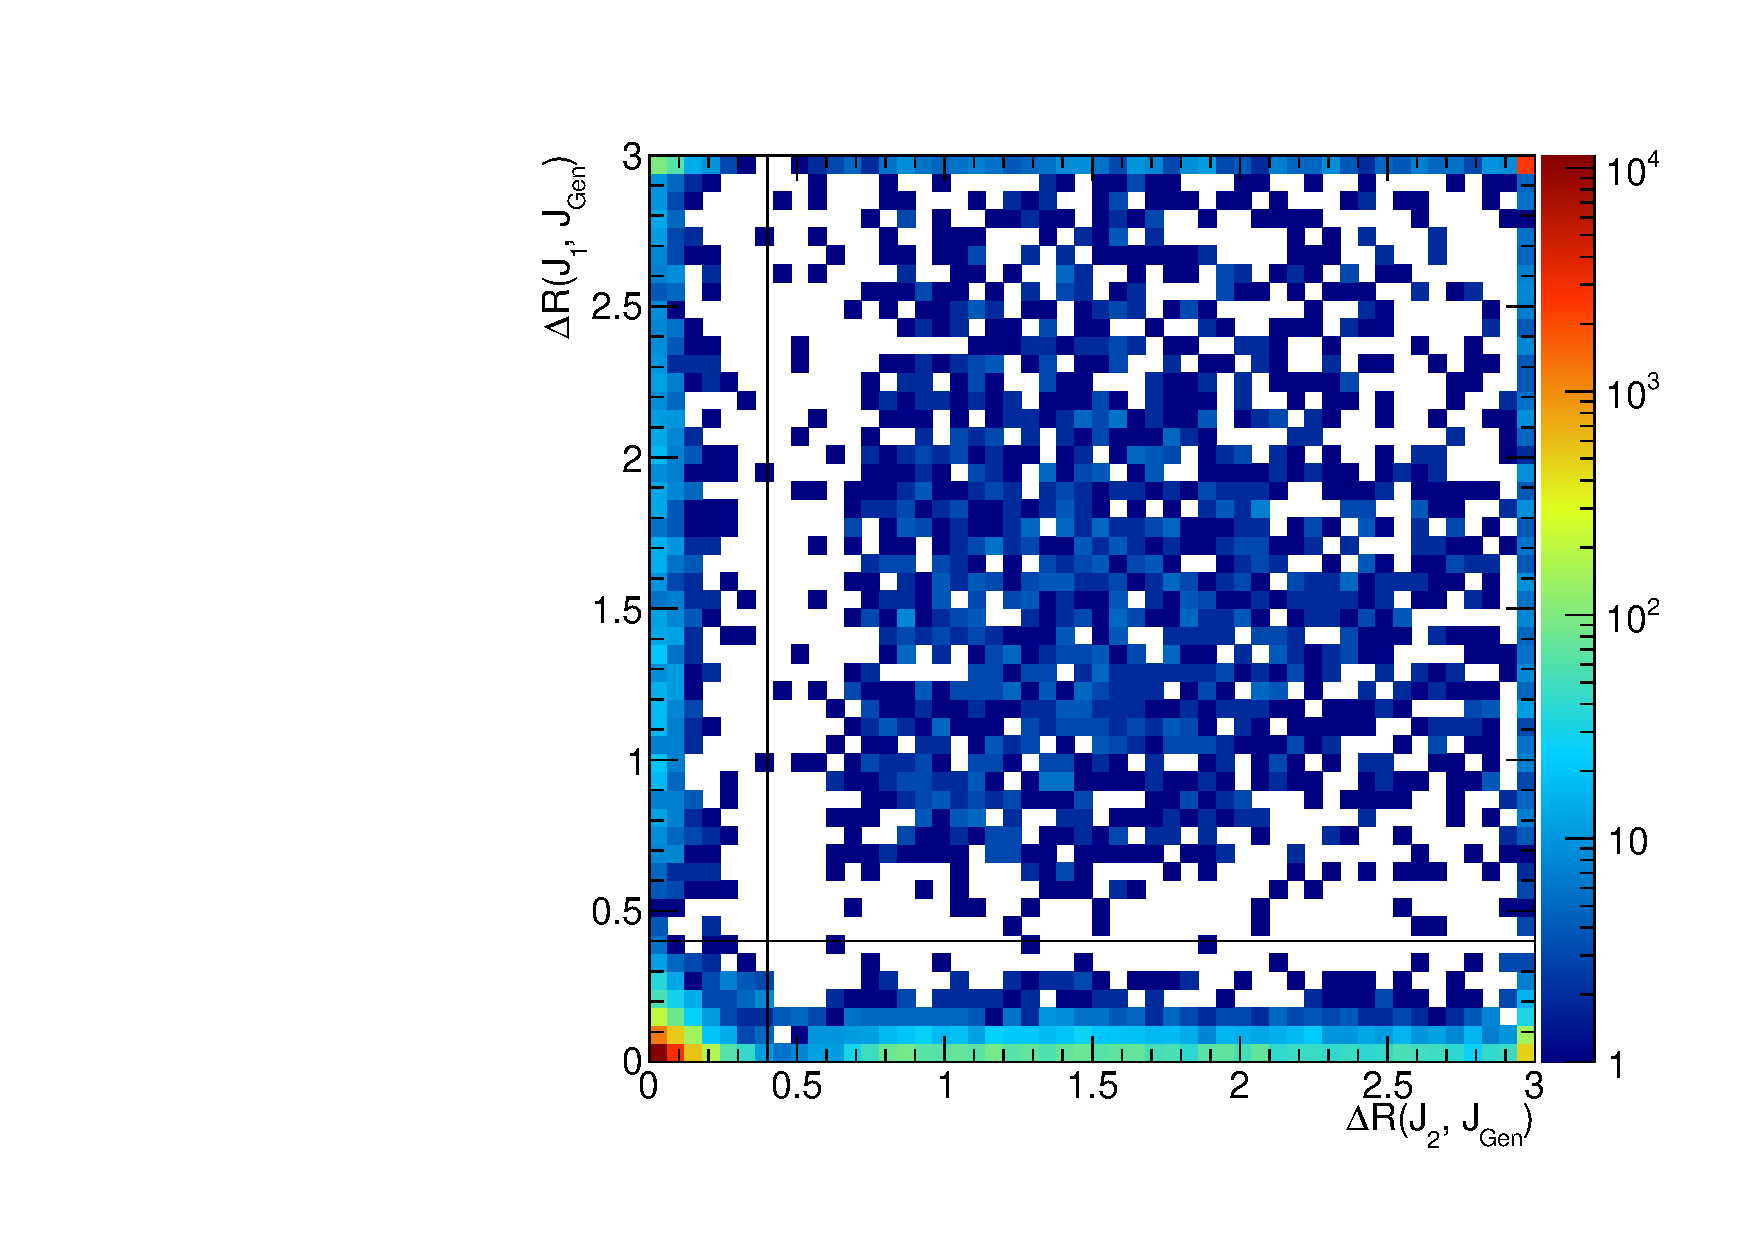
\includegraphics[width=0.6\textwidth]{plots/2D_drgen.pdf}
\end{tabular}
\caption{The $\Delta$R(jet1, genjet) vs. $\Delta$R(jet2, genjet)
\label{fig:2Ddrplot}
}
\end{center}
\end{figure}

We label the sections on this plot starting from the top left and going clockwise as sections 1 through 4. The events with 2 hard scatter jets are represented in section 4, the section with 1 hard scatter jet and 1 PU jet are represented in sections 1 and 3, adn the events with 2 PU jets are represented in section 2. Now we will look at $\Delta\phi$ between the 2 lead jets to see if we can better understand the events.

\subsection{$\Delta\phi$ Between the Two Jets}
In Fig.~\ref{fig:dphiplots}, we show the distribution of the $\Delta\phi$ between the two highest pt jets in the event. 

%% delta phi plots
\begin{figure}[!hbtp]
\centering
\subfigure[]{
\centering
\label{subfig:dphisamecut}
%% \includegraphics[width=.4\textwidth]{/home/users/cwelke/public_html/Zmet/jetstudy/pdf/dphij1j2_jet1_jet2drgen_Selection.pdf}
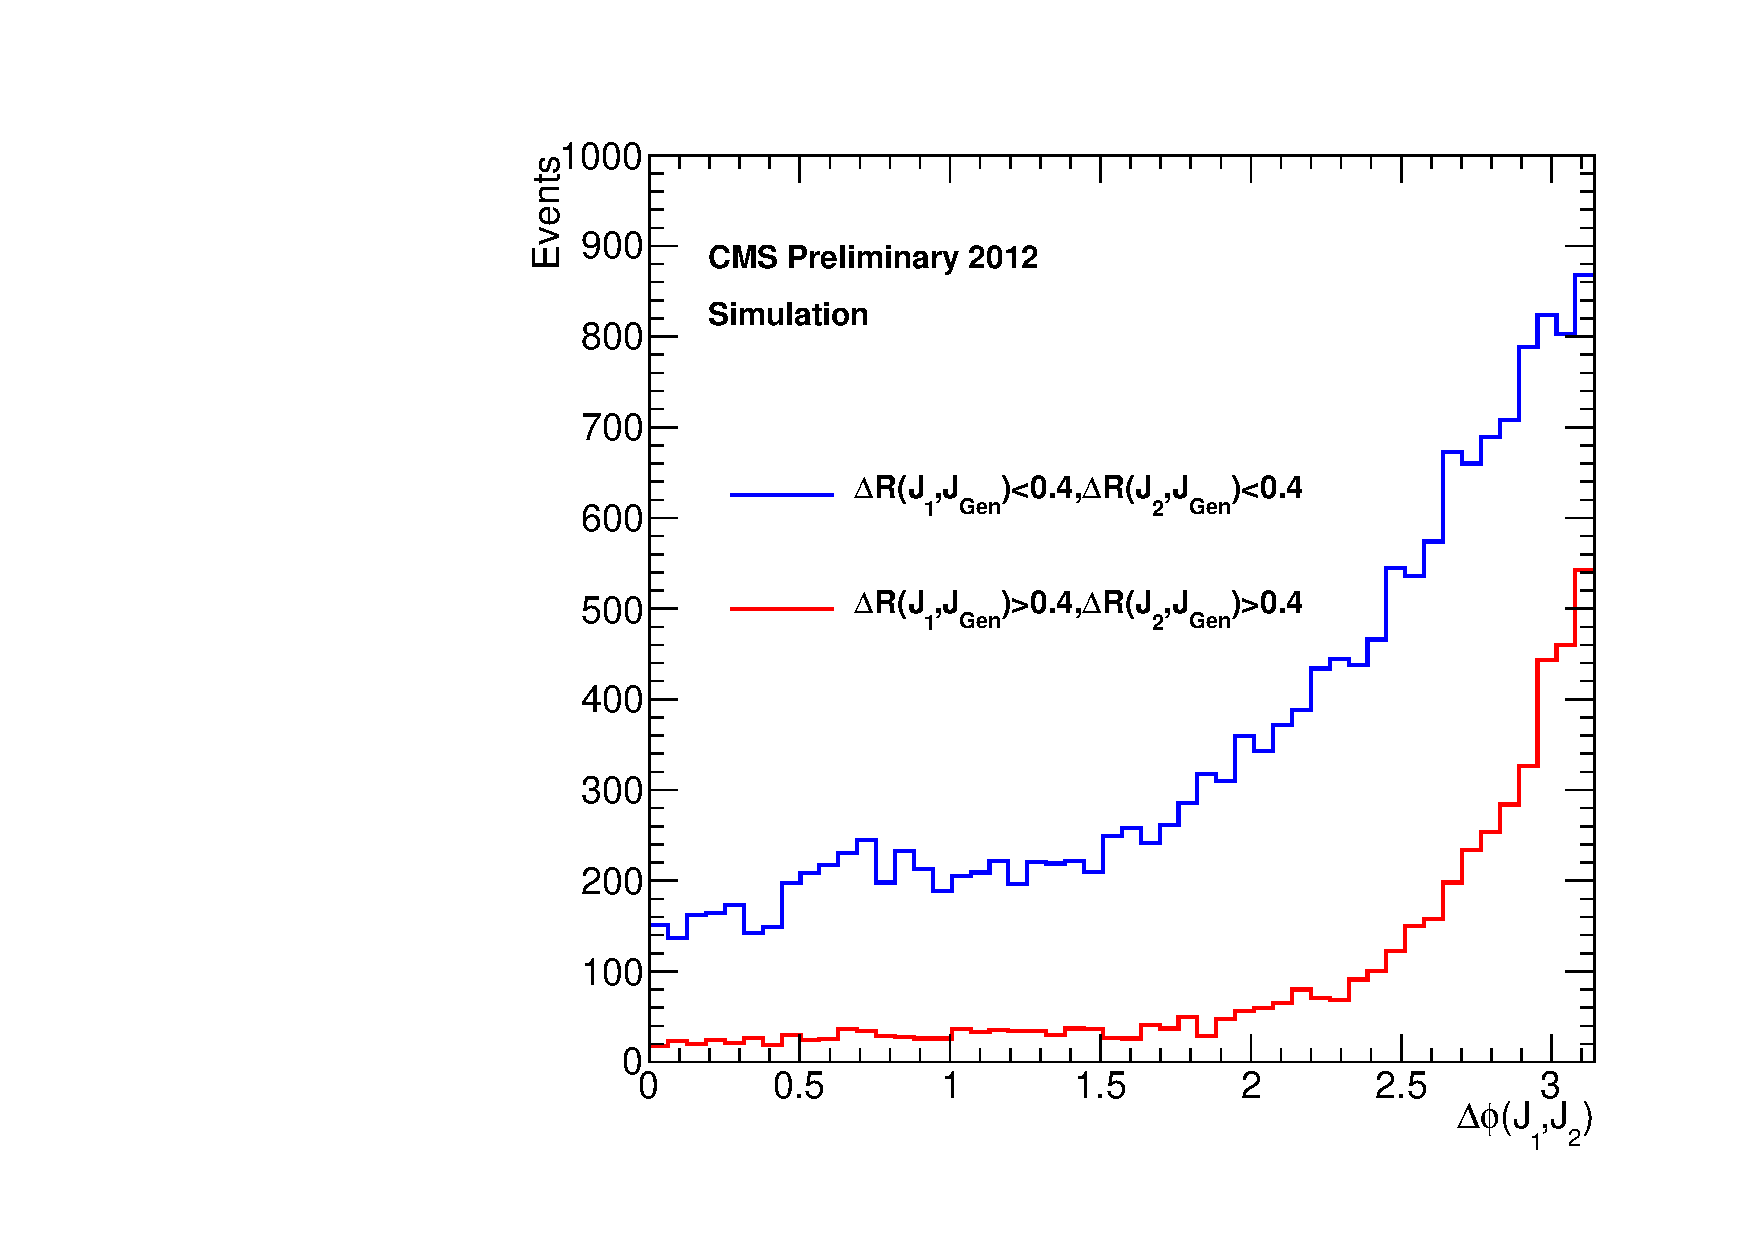
\includegraphics[width=.4\textwidth]{plots/dphi_jet1_jet2.pdf}
}
\subfigure[]{
\centering
\label{subfig:dphianticut}
%% \includegraphics[width=.4\textwidth]{/home/users/cwelke/public_html/Zmet/jetstudy/pdf/dphij1j2_All_Selection.pdf}
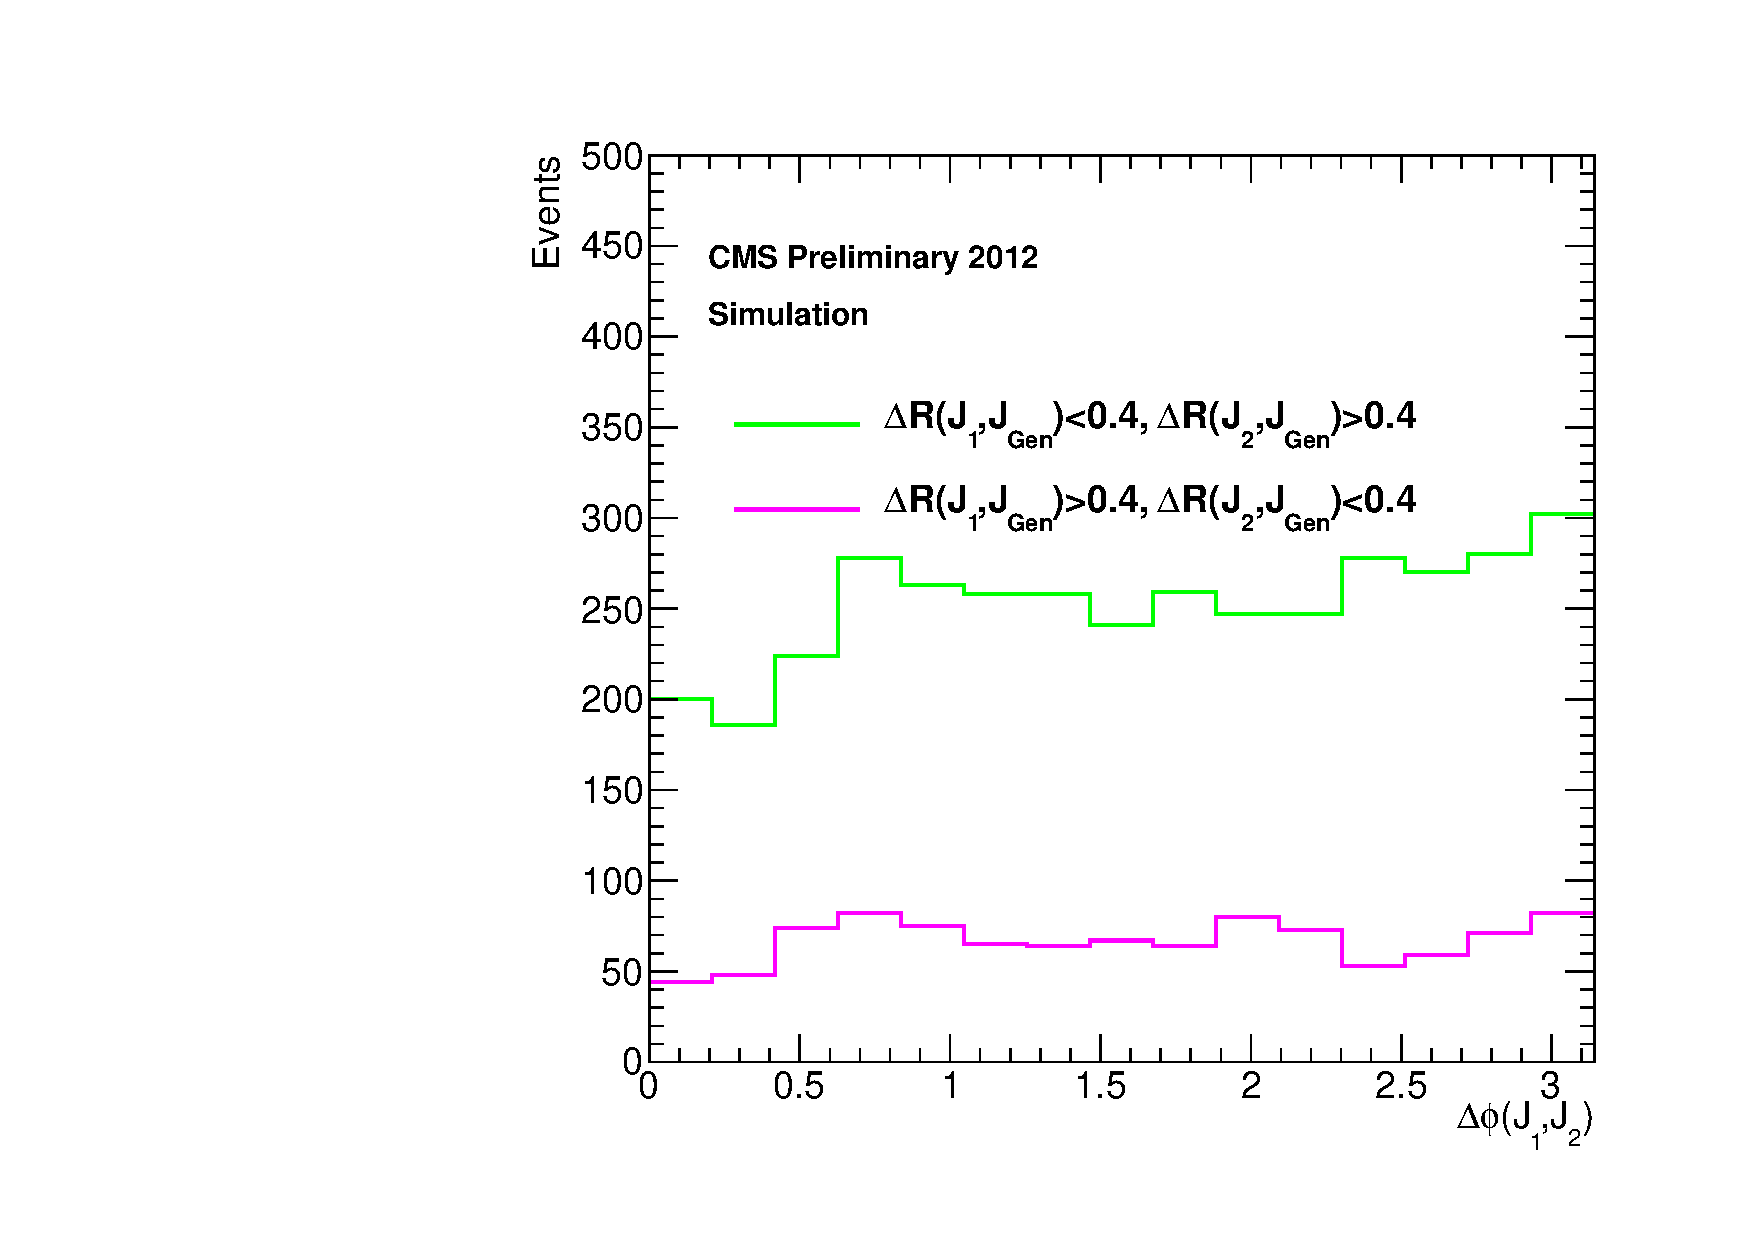
\includegraphics[width=.4\textwidth]{plots/dphi_jet1_antijet2.pdf}
}\\
\caption{The $\Delta\phi$ distribution between the two leading jets is shown in blue where both jets are matched to gen jets and shown in red for events where both jets are from PU in \subref{subfig:dphisamecut} and in \subref{subfig:jet12cut} one jet is matched to a gen jet and the other jet is not matched to a gen jet.}
\label{fig:dphiplots}
\end{figure}

These distributions represent the various sections in Fig.~\ref{fig:2Ddrplot} as follows, section 1 is magenta, section 2 is red, section 3 is green, and section 4 is blue. 
The events in section 2 show a strong correlation for events to be back to back. The events in sections 1 and 3 show a flat distribution which implies that the jets $\phi$ is uncorrelated. 

\clearpage

\section{Event Preselection}
\label{sec:eventSel}
The purpose of the preselection is to reject backgrounds other than 
$t\bar{t} \to$ dileptons.  We compare the kinematical 
properties of this sample with expectations from $t\bar{t}$ 
Monte Carlo.

The preselection is based on the 
$t\bar{t}$ analysis~\cite{ref:top}.  
We select events with two opposite sign, well-identified and isolated
leptons ($ee$, $e\mu$, or $\mu\mu$); one of the leptons must 
have $P_T > 20$ GeV,
the other one must have $P_T > 10$ GeV. Events with dilepton mass
consistent with $Z \to ee/\mu\mu$ are rejected.
In case of events with 
more than two such leptons, we select the pair that maximizes the scalar 
sum of lepton $P_T$'s.
There must be at least two 
pfjets of $P_T > 30$ GeV and $|\eta| < 3.0$;  jets must pass
loose {\tt pfJetId} and be separated by $\Delta R >$ 0.4 from any 
lepton with $P_T > 10$~GeV passing the selection.
The scalar sum \Ht\ of the 
$P_T$ of all such jets must exceed 100 GeV, for the dilepton-\Ht\ sample
this requirement is increased to 200 GeV since these triggers have large inefficiency
below this threshold.
Finally $\met > 50$ GeV (we use pfmet). More details are given in the subsections below.

\subsection{Event Cleanup}
\label{sec:cleanup}

\begin{itemize}
   \item Require at least one good deterministic annealing (DA) vertex
   \begin{itemize}
      \item not fake
      \item ndof $>$ 4
      \item $|\rho| < 2$ cm
      \item $|z| < 24$ cm.  
   \end{itemize}
\end{itemize}


\subsection{Muon Selection}
\label{sec:muon}

Muon candidates are RECO muon objects passing the following
requirements:

\begin{itemize}

\item $p_{T} > 5$~GeV and $|\eta| < 2.4$

\item Global Muon and Tracker Muon

\item $\chi^2$/ndof of global fit $<$ 10

\item At least 11 hits in the tracker fit

\item Impact parameter with respect to the first DA vertex $d_{0} < 200$~$\mu$m and $d_{z} < 1$~cm

\item $Iso \equiv E_T^{\rm iso}/p_T < $~0.15, $E_T^{\rm iso}$ is defined as the sum of 
transverse energy/momentum deposits in ecal, hcal, and tracker, in a cone of 0.3

\item At least one of the hits from the 
standalone muon must be used in the global fit

\item Require tracker $\Delta p_T/p_T < 0.1$. This cut was not in the original top analysis.
It is motivated by the observation of poorly measured muons in data with large
relative $p_T$ uncertainty, giving significant contributions to the \met

\item {\color{red} \bf LIST FO DEFINITIONS HERE? }

\end{itemize}



\subsection{Electron Selection}
\label{sec:electron}

Electron candidates are RECO GSF electrons passing the following requirements:

\begin{itemize}

\item $p_{T}>10$~GeV and $|\eta| < 2.5$.

\item Veto electrons with a supercluster in the transition region $1.4442 < |\eta| < 1.556$.

\item VBTF90 identification\cite{ref:vbtf} with requirements tightened to match the CaloIdT and TrkIdVL HLT requirements:

  \begin{itemize}
  \item $\sigma_{i\eta i\eta} < $ 0.01 (EB), 0.03 (EE)
  \item $\Delta\phi < $ 0.15 (EB), 0.10 (EE)
  \item $\Delta\eta < $ 0.007 (EB), 0.009 (EE)
  \item $H/E < $ 0.1 (EB), 0.075 (EE)
  \end{itemize}  

\item Impact parameter with respect to the first DA vertex $d_0 < 400$~$\mu$m and $d_z < 1$~cm.

\item $Iso \equiv $ $E_T^{\rm iso}/p_T < $ 0.15.  $E_T^{\rm iso}$
is defined as the sum of transverse energy/momentum deposits in ecal,
hcal, and tracker, in a 
cone of 0.3.  A 1 GeV pedestal is subtracted from the ecal energy 
deposition in the EB, however the ecal energy is never allowed to 
go negative.

\item Electrons with a tracker or global muon within $\Delta R$ of 
0.1 are vetoed.

\item The number of missing expected inner hits must be less than 
two~\cite{ref:conv}.

\item Conversion removal via partner track finding: any electron
where an additional GeneralTrack is found with $Dist < 0.02$ cm 
and $\Delta \cot \theta < 0.02$ is vetoed~\cite{ref:conv}.

%\item Cleaning for ECAL spike (aka Swiss-Cross cleaning) has been applied
%at the reconstruction level (CMSSW 38x).

\item {\color{red} \bf LIST FO DEFINITIONS HERE? }

\end{itemize}

\subsection{Invariant mass requirement}
\label{sec:zveto}

We remove $e^+e^-$ and $\mu^+ \mu^-$ events with invariant 
mass between 76 and 106 GeV.  We also remove events
with invariant mass $<$ 12 GeV, since this kinematical region is 
not well reproduced in CMS Monte Carlo and to remove Upsilons.

In addition, we remove $Z \to \mu\mu\gamma$
candidates with the $\gamma$ collinear with one of the muons.  This is
done as follows:
if the ecal energy associated with one of the muons is greater than 6 GeV,
we add this energy to the momentum of the initial muon, and we recompute
the $\mu\mu$ mass.  If this mass is between 76 and 106 GeV, the event is rejected.


\subsection{Trigger Selection}
\label{sec:trigSel}

We do not make any requirements on HLT bits in the Monte Carlo.
Instead, as discussed in 
Section~\ref{sec:trgEff}, a trigger efficiency weight is applied
to each event, based on the trigger efficiencies measured on data (see Sec.~\ref{sec:trgEff}).

We select data events using the following triggers. An event in the $ee$ channel is required
to pass a DoubleElectron trigger, an event in the $\mu\mu$ channel is required to pass a 
DoubleMu trigger, and an event in the $e\mu$ channel is required to pass a Ele-Mu trigger.

   \begin{itemize}
      \item High \pt\ dilepton trigger sample
      \begin{itemize}
         \item \verb=HLT_Ele17_CaloIdL_CaloIsoVL_Ele8_CaloIdL_CaloIsoVL=
         \item {\footnotesize \verb=HLT_Ele17_CaloIdT_TrkIdVL_CaloIsoVL_TrkIsoVL_Ele8_CaloIdT_TrkIdVL_CaloIsoVL_TrkIsoVL=}
         \item \verb=HLT_DoubleMu7=
         \item \verb=HLT_Mu13_Mu7=
         \item \verb=HLT_Mu17_Ele8_CaloIdL=
         \item \verb=HLT_Mu8_Ele17_CaloIdL=
      \end{itemize}
      \item Lepton \Ht\ cross trigger sample
      \begin{itemize}
        \item \verb=HLT_DoubleMu3_HT150=
        \item \verb=HLT_DoubleMu3_HT160=
        \item \verb=HLT_Mu3_Ele8_CaloIdL_TrkIdVL_HT150=
        \item \verb=HLT_Mu3_Ele8_CaloIdT_TrkIdVL_HT150=
        \item \verb=HLT_Mu3_Ele8_CaloIdL_TrkIdVL_HT160=
        \item \verb=HLT_Mu3_Ele8_CaloIdT_TrkIdVL_HT160=
        \item \verb=HLT_DoubleEle8_CaloIdL_TrkIdVL_HT150=
        \item \verb=HLT_DoubleEle8_CaloIdT_TrkIdVL_HT150=
        \item \verb=HLT_DoubleEle8_CaloIdL_TrkIdVL_HT160=
        \item \verb=HLT_DoubleEle8_CaloIdT_TrkIdVL_HT160=
      \end{itemize}
   \end{itemize}









%\section{Preselection yields}
%\label{sec:yields}

The data yields and corresponding MC predictions after this event preselection
are given in Table~\ref{tab:yields}. The MC yields are normalized to~\lumifinal\ using 
next-to-leading order (NLO) cross sections. At the current LHC luminosity, the mean
number of interactions in a single beam crossing is approximately 5. In the MC, multiple interactions
are superimposed on the hard collision, and the MC is reweighted such that the distribution
of reconstructed primary vertices matches that in data. As expected, the MC predicts that the 
sample passing the preselection is dominated by dilepton $t\bar{t}$. The data yield is in 
reasonable agreement~\footnote{The luminosity is currently underestimated by approximately 10\%,
which explains the observed excess in data. The estimate will be updated before EPS.}
 with the prediction. We also quote the yields for
the LM1 and LM3 benchmark scenarios.

\begin{table}[htb]
\begin{center}
\caption{\label{tab:yields} Data yields and MC predictions after preselection, using the quoted NLO production cross sections $\sigma$.
The \ttll\ corrresponds  to dilepton $t\bar{t}$, including 
$t \to W \to \tau \to \ell$; \ttfake\ includes all other $t\bar{t}$ decay modes. 
The samples of MC $t\bar{t}$, $W^{\pm}$ + jets, and single-top events were 
generated with \MADGRAPH. The Drell--Yan sample (which includes events with
invariant masses as low as 10\GeVcc) was generated using a mixture of \MADGRAPH\ and 
\PYTHIA  and includes decays to the $\tau^+\tau^-$ final state. All other samples were generated with \PYTHIA. 
The LM1 and LM3 benchmark scenarios are defined in the text; the quoted $\sigma$ values refer to the total production
cross section for SUSY particles in these scenarios. Uncertainties are statistical only.
}
\vspace{2 mm}
\begin{tabular}{lr|cccc}
\hline
         Sample     & $\sigma$ [pb]  &            $ee$   &       $\mu\mu$   &         $e\mu$   &       total  \\
\hline
          \ttll     &     17 & 147.6 $\pm$ 3.2   &166.4 $\pm$ 3.2   &391.7 $\pm$ 5.1   &705.8 $\pm$ 6.8  \\
        \ttfake     &    141 &   4.5 $\pm$ 0.6   &  1.3 $\pm$ 0.3   &  8.1 $\pm$ 0.7   & 13.9 $\pm$ 1.0  \\
DY$\to\ell^+\ell^-$ &  16677 &   6.6 $\pm$ 1.8   &  9.5 $\pm$ 2.1   & 13.4 $\pm$ 2.6   & 29.6 $\pm$ 3.8  \\
            \WW     &     43 &   1.4 $\pm$ 0.2   &  1.5 $\pm$ 0.2   &  3.4 $\pm$ 0.2   &  6.3 $\pm$ 0.3  \\
            \WZ     &     18 &   0.3 $\pm$ 0.0   &  0.4 $\pm$ 0.0   &  0.7 $\pm$ 0.1   &  1.3 $\pm$ 0.1  \\
            \ZZ     &    5.9 &   0.1 $\pm$ 0.0   &  0.1 $\pm$ 0.0   &  0.2 $\pm$ 0.0   &  0.4 $\pm$ 0.0  \\
     single top     &    102 &   4.5 $\pm$ 0.2   &  5.0 $\pm$ 0.2   & 11.9 $\pm$ 0.3   & 21.4 $\pm$ 0.5  \\
         \wjets     &  96648 &   4.5 $\pm$ 1.9   &  0.0 $\pm$ 0.0   &  2.8 $\pm$ 1.7   &  7.3 $\pm$ 2.6  \\
\hline
    total SM MC     &        & 169.7 $\pm$ 4.2   &184.3 $\pm$ 3.9   &432.2 $\pm$ 6.0   &786.1 $\pm$ 8.3  \\
\hline
           data     &        &             193   &            201   &            485   &            879  \\
\hline
            LM1     &    6.7 &  22.3 $\pm$ 0.6   & 24.8 $\pm$ 0.6   & 12.8 $\pm$ 0.4   & 59.9 $\pm$ 0.9  \\
            LM3     &    5.3 &   7.9 $\pm$ 0.3   &  9.6 $\pm$ 0.3   & 14.2 $\pm$ 0.4   & 31.7 $\pm$ 0.6  \\
\hline
\end{tabular}
\end{center}
\end{table}


%\clearpage
\section{Background Estimation Techniques}
\label{sec:bkg}

In this section we describe the techniques used to estimate the SM backgrounds in our signal regions defined by requirements of large \MET.
The SM backgrounds fall into three categories:

\begin{itemize}
\item \zjets: this is the dominant background after the preselection. The \MET\ in \zjets\ events is estimated with the 
``\MET\ templates'' technique described in Sec.~\ref{sec:bkg_zjets};
\item Flavor-symmetric (FS) backgrounds: this category includes processes which produces 2 leptons of uncorrelated flavor. It is dominated
by \ttbar\ but also contains Z$\to\tau\tau$, WW, and single top processes. This is the dominant contribution in the signal regions, and it
is estimated using a data control sample of e$\mu$ events as described in Sec.~\ref{sec:bkg_fs};
\item WZ and ZZ backgrounds: this background is estimated from MC, after validating the MC modeling of these processes using data control
samples with jets and exactly 3 leptons (WZ control sample) and exactly 4 leptons (ZZ control sample) as described in Sec.~\ref{sec:bkg_vz};
%\item Rare SM backgrounds: this background contains rare processes such as $t\bar{t}$V and triple vector boson processes VVV (V=W,Z).
%This background is estimated from MC as described in Sec.~\ref{sec:bkg_raresm}. {\bf FIXME: add rare MC}
\end{itemize}

\subsection{Estimating the \zjets\ Background with \MET\ Templates}
\label{sec:bkg_zjets}

The premise of this data driven technique is that \MET\ in \zjets\ events
is produced by the hadronic recoil system and {\it not} by the leptons making up the Z.
Therefore, the basic idea of the \MET\ template method is to measure the \MET\ distribution in 
a control sample which has no true MET and the same general attributes regarding
fake MET as in \zjets\ events. We thus use a sample of \gjets\ events, since both \zjets\
and \gjets\ events consist of a well-measured object recoiling against hadronic jets.

For selecting photon-like objects, the very loose photon selection described in Sec.~\ref{sec:phosel} is used.
It is not essential for the photon sample to have high purity. For our purposes, selecting jets with predominantly 
electromagnetic energy deposition in a good fiducial volume suffices to ensure that 
they are well measured and do not contribute to fake \MET. The \gjets\ events are selected with a suite of
single photon triggers with \pt thresholds varying from 22--90 GeV. The events are weighted by the trigger prescale
such that \gjets\ events evenly sample the conditions over the full period of data taking.
There remains a small difference in the PU conditions in the \gjets\ vs. \zjets\ samples due to the different
dependencies of the $\gamma$ vs. Z isolation efficiencies on PU. To account for this, we reweight the \gjets\ samples
to match the distribution of reconstructed primary vertices in the \zjets\ sample.

To account for kinematic differences between the hadronic systems in the control vs. signal 
samples, we measure the \MET\ distributions in the \gjets\ sample in bins of the number of jets 
and the scalar sum of jet transverse energies (\Ht). These \MET\ templates are extracted separately from the 5 single photon
triggers with thresholds 22, 36, 50, 75, and 90 GeV, so that the templates are effectively binned in photon \pt.
All \MET distributions are normalized to unit area to form ``MET templates''.
The prediction of the MET in each \Z event is the template which corresponds to the \njets,
\Ht, and Z \pt in the \zjets\ event. The prediction for the \Z sample is simply the sum of all such templates.
All templates are displayed in App.~\ref{app:templates}.

After preselection, there is  a small contribution from backgrounds other than \zjets. To correct for this, the \MET\ templates
prediction is scaled such that the total background prediction matches the observed data yield in the \MET\ 0--60 GeV region.
Because the non-\zjets impurity in the low \MET\ region after preselection is very small, this results in 
scaling factors of 0.985 (0.995) for the inclusive (targeted) search.

\subsection{Estimating the Flavor-Symmetric Background with e$\mu$ Events}
\label{sec:bkg_fs}

In this subsection we describe the background estimate for the FS background. Since this background produces equal rates of same-flavor (SF)
ee and $\mu\mu$ lepton pairs as opposite-flavor (OF) e$\mu$ lepton pairs, the OF yield can be used to estimate the SF yield, after
correcting for the different electron vs. muon offline selection efficiencies and the different efficiencies for the ee, $\mu\mu$, and e$\mu$ triggers.

An important quantity needed to translate from the OF yield to a prediction for the background in the SF final state is the ratio 
$R_{\mu e} = \epsilon_\mu / \epsilon_e$, where $\epsilon_\mu$ ($\epsilon_e$) indicates the offline muon (electron) selection efficiency. 
This quantity can be extracted from data using the observed Z$\to\mu\mu$ and Z$\to$ee yields in the preselection region, after correcting 
for the different trigger efficiencies.

Hence we define:

\begin{itemize}
\item $N_{ee}^{\rm{trig}} = \epsilon_{ee}^{\rm{trig}}N_{ee}^{\rm{offline}}$,
\item $N_{\mu\mu}^{\rm{trig}} = \epsilon_{\mu\mu}^{\rm{trig}}N_{\mu\mu}^{\rm{offline}}$,
\item $N_{e\mu}^{\rm{trig}} = \epsilon_{e\mu}^{\rm{trig}}N_{e\mu}^{\rm{offline}}$.
\end{itemize}
 
Here $N_{\ell\ell}^{\rm{trig}}$ denotes the number of selected Z events in the $\ell\ell$ channel passing the offline and trigger selection
(in other words, the number of recorded and selected events), $\epsilon_{\ell\ell}^{\rm{trig}}$ is the trigger efficiency, and 
$N_{\ell\ell}^{\rm{offline}}$ is the number of events that would have passed the offline selection if the trigger had an efficiency of 100\%.
Thus we calculate the quantity:

\begin{equation}
R_{\mu e} = \sqrt{\frac{N_{\mu\mu}^{\rm{offline}}}{N_{ee}^{\rm{offline}}}} = \sqrt{\frac{N_{\mu\mu}^{\rm{trig}}/\epsilon_{\mu\mu}^{\rm{trig}}}{N_{ee}^{\rm{trig}}/\epsilon_{ee}^{\rm{trig}}}} 
= \sqrt{\frac{304953/0.88}{239661/0.95}} = 1.17\pm0.07.
\end{equation}

Here we have used the Z$\to\mu\mu$ and Z$\to$ee yields from Table~\ref{table:zyields_2j} and the trigger efficiencies quoted in Sec.~\ref{sec:datasets}.
The indicated uncertainty is due to the 3\% uncertainties in the trigger efficiencies. %{\bf FIXME: check for variation w.r.t. lepton \pt}.
The predicted yields in the ee and $\mu\mu$ final states are calculated from the observed e$\mu$ yield as

\begin{itemize}
\item $N_{ee}^{\rm{predicted}}    = \frac {N_{e\mu}^{\rm{trig}}} {\epsilon_{e\mu}^{\rm{trig}}} \frac {\epsilon_{ee}^{\rm{trig}}} {2 R_{\mu e}} 
= \frac{N_{e\mu}^{\rm{trig}}}{0.92}\frac{0.95}{2\times1.17} = (0.44\pm0.05) \times N_{e\mu}^{\rm{trig}}$ ,
\item $N_{\mu\mu}^{\rm{predicted}} = \frac {N_{e\mu}^{\rm{trig}}} {\epsilon_{e\mu}^{\rm{trig}}} \frac {\epsilon_{\mu\mu}^{\rm{trig}} R_{\mu e}}  {2}
= \frac {N_{e\mu}^{\rm{trig}}} {0.95} \frac {0.88 \times 1.17}{2} = (0.54\pm0.07) \times N_{e\mu}^{\rm{trig}}$,
\end{itemize}

and the predicted yield in the combined ee and $\mu\mu$ channel is simply the sum of these two predictions:

\begin{itemize}
\item $N_{ee+\mu\mu}^{\rm{predicted}} = (0.98\pm0.06)\times N_{e\mu}^{\rm{trig}}$.
\end{itemize}

Note that the relative uncertainty in the combined ee and $\mu\mu$ prediction is smaller than those for the individual ee and $\mu\mu$ predictions
because the uncertainty in $R_{\mu e}$ cancels when summing the ee and $\mu\mu$ predictions. %{\bf N.B. these uncertainties are preliminary}.

To improve the statistical precision of the FS background estimate, we remove the requirement that the e$\mu$ lepton pair falls in the Z mass window.
Instead we scale the e$\mu$ yield by $K$, the efficiency for e$\mu$ events to satisfy the Z mass requirement, extracted from simulation. In Fig.~\ref{fig:K_incl}
we display the value of $K$ in data and simulation, for a variety of \MET\ requirements, for the inclusive analysis. 
Based on this we chose $K=0.14\pm0.02$ for the lower \MET\ regions, $K=0.14\pm0.04$ for the \MET\ $>$ 200 GeV region,and $K=0.14\pm0.09$ for \MET\ $>$ 300 GeV,
where the larger uncertainties reflect the reduced statistical precision at large \MET.
The corresponding plot for the targeted analysis, including the b-veto, is displayed in Fig.~\ref{fig:K_targeted}.
Based on this we chose $K=0.13\pm0.02$
for all \MET\ regions up to  \MET\ $>$ 150 GeV. For the \MET\ $>$ 200 GeV region we choose $K=0.13\pm0.05$, due to the reduced  statistical precision.

\begin{figure}[!ht]
\begin{center}
\begin{tabular}{cc}
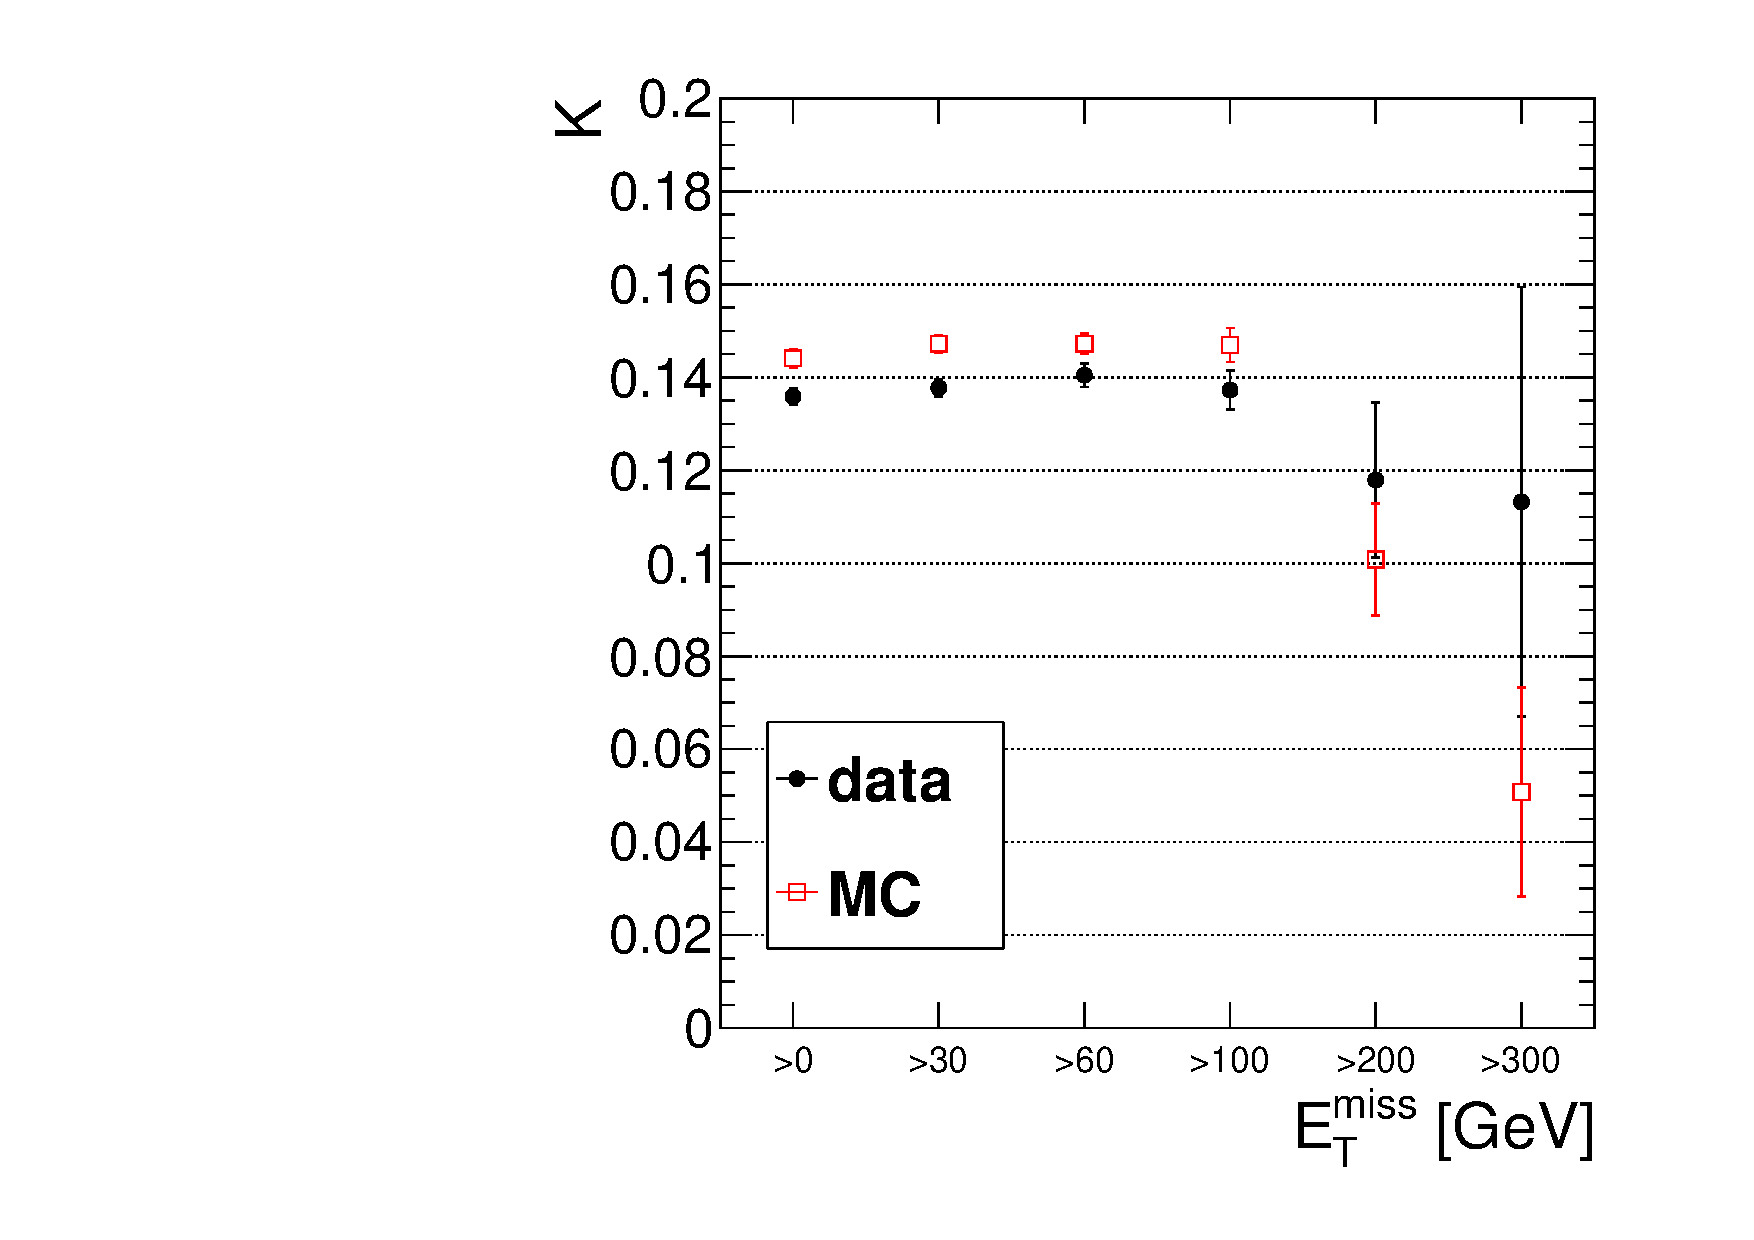
\includegraphics[width=0.4\textwidth]{plots/extractK_inclusive_19fb.pdf} &
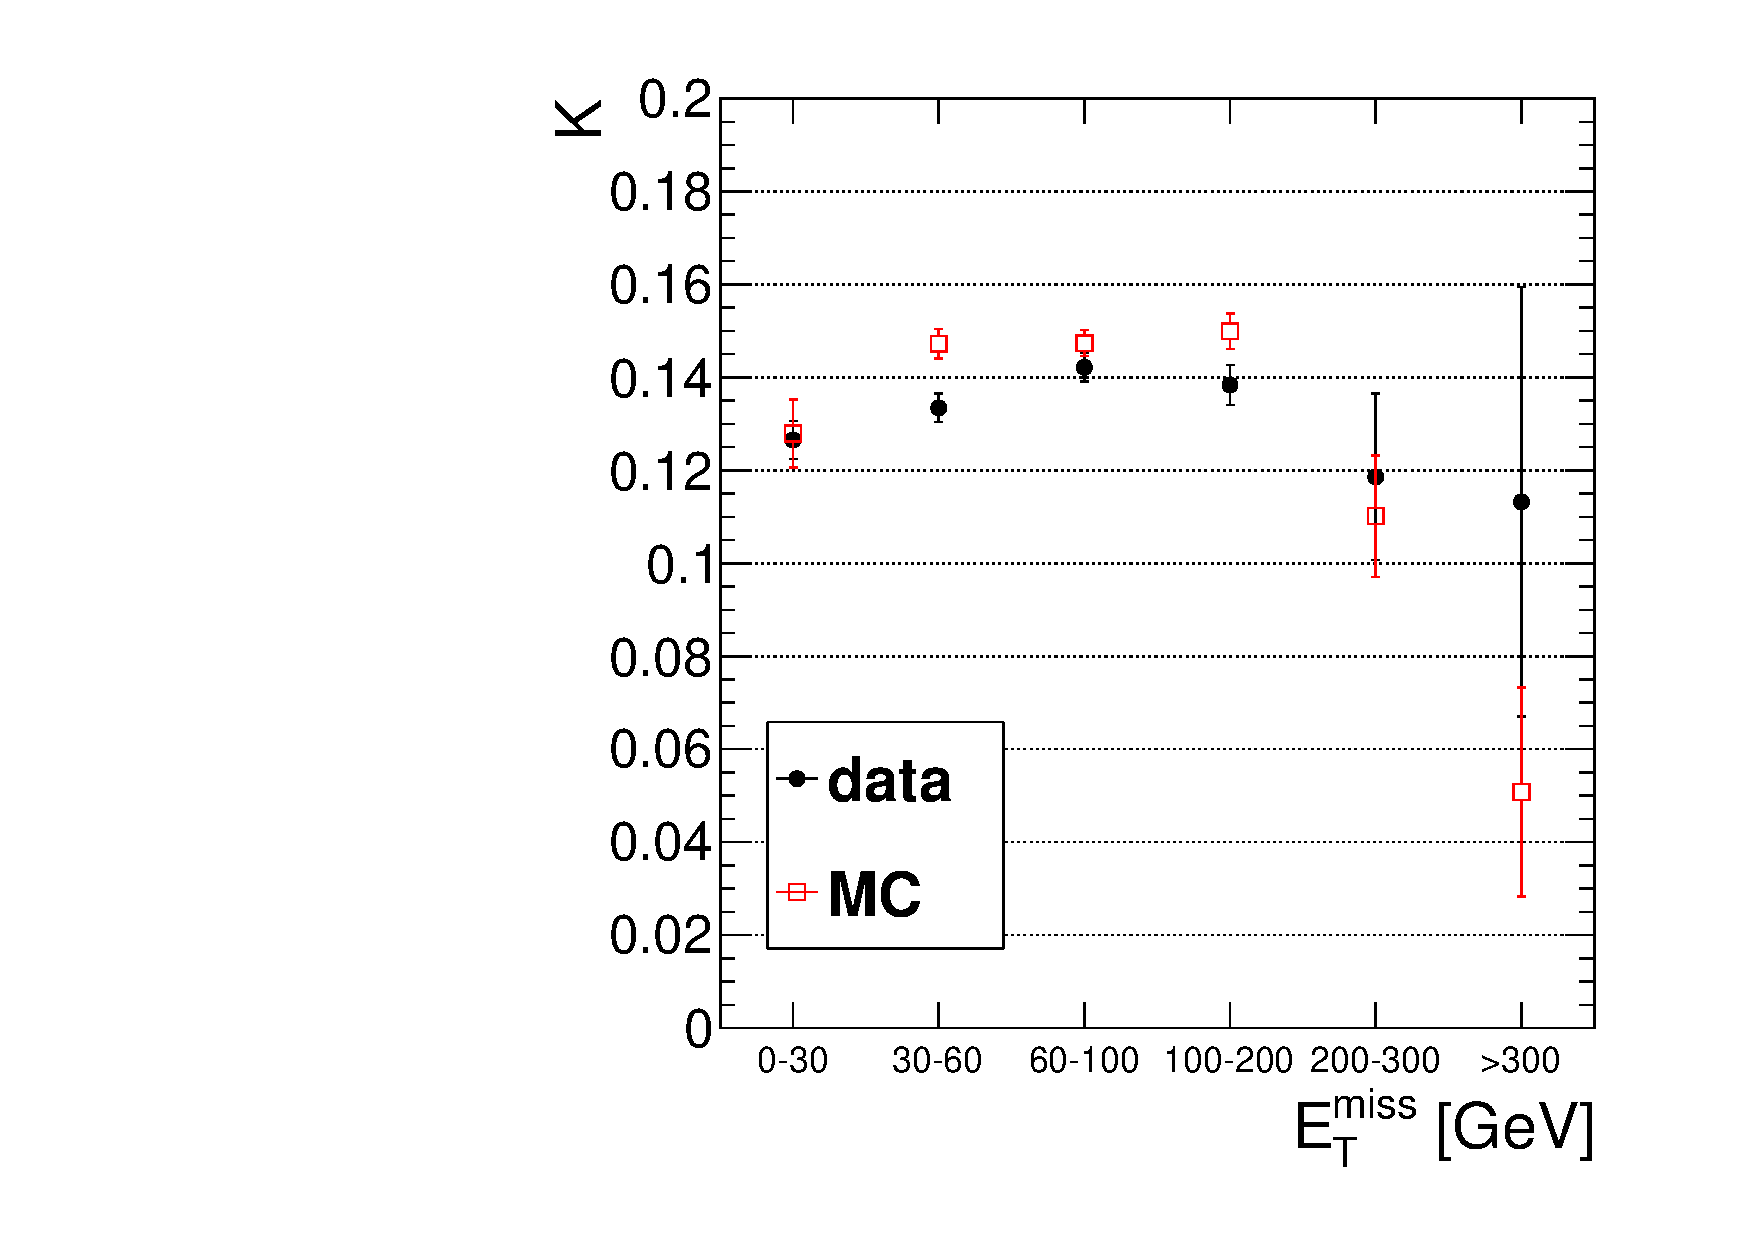
\includegraphics[width=0.4\textwidth]{plots/extractK_exclusive_19fb.pdf} \\
\end{tabular}
\caption{\label{fig:K_incl}
The efficiency for e$\mu$ events to satisfy the dilepton mass requirement, $K$, in data and simulation for inclusive \MET\ intervals (left) and
exclusive \MET\ intervals (right) for the inclusive analysis. 
}

\begin{comment}

----------------------------------------
  EXCLUSIVE RESULTS
----------------------------------------

Using selection : ((((leptype==2)&&(csc==0 && hbhe==1 && hcallaser==1 && ecaltp==1 && trkfail==1 && eebadsc==1 && hbhenew==1))&&(isdata==0 || (run<197556 || run>198913)))&&(njets>=2))&&(lep1.pt()>20 && lep2.pt()>20)
Using weight    : vtxweight * weight
OF entries (total)  44537
OF entries (Z mass) 6051
K                   0.135865
Warning in <TROOT::Append>: Replacing existing TH1: htot (Potential memory leak).
Warning in <TROOT::Append>: Replacing existing TH1: hZ (Potential memory leak).

--------------------------------------------------------------
pfmet>0   && pfmet<30

data  : 
total : 7563
Z     : 957
K     : 0.13 +/- 0.004

MC    : 
total : 399.019
Z     : 51.0493
K     : 0.13 +/- 0.007
--------------------------------------------------------------


--------------------------------------------------------------
pfmet>30  && pfmet<60

data  : 
total : 14185
Z     : 1893
K     : 0.13 +/- 0.003

MC    : 
total : 755.309
Z     : 111.206
K     : 0.15 +/- 0.003
--------------------------------------------------------------


--------------------------------------------------------------
pfmet>60  && pfmet<100

data  : 
total : 14928
Z     : 2122
K     : 0.14 +/- 0.003

MC    : 
total : 838.418
Z     : 123.554
K     : 0.15 +/- 0.003
--------------------------------------------------------------


--------------------------------------------------------------
pfmet>100 && pfmet<200

data  : 
total : 7437
Z     : 1029
K     : 0.14 +/- 0.004

MC    : 
total : 451.624
Z     : 67.7098
K     : 0.15 +/- 0.004
--------------------------------------------------------------


--------------------------------------------------------------
pfmet>200 && pfmet<300

data  : 
total : 371
Z     : 44
K     : 0.12 +/- 0.018

MC    : 
total : 24.2441
Z     : 2.67077
K     : 0.11 +/- 0.013
--------------------------------------------------------------


--------------------------------------------------------------
pfmet>300

data  : 
total : 53
Z     : 6
K     : 0.11 +/- 0.046

MC    : 
total : 4.53108
Z     : 0.230071
K     : 0.05 +/- 0.022
--------------------------------------------------------------


----------------------------------------
  INCLUSIVE RESULTS
----------------------------------------

Using selection : ((((leptype==2)&&(csc==0 && hbhe==1 && hcallaser==1 && ecaltp==1 && trkfail==1 && eebadsc==1 && hbhenew==1))&&(isdata==0 || (run<197556 || run>198913)))&&(njets>=2))&&(lep1.pt()>20 && lep2.pt()>20)
Using weight    : vtxweight * weight
OF entries (total)  44537
OF entries (Z mass) 6051
K                   0.135865
Warning in <TROOT::Append>: Replacing existing TH1: htot (Potential memory leak).
Warning in <TROOT::Append>: Replacing existing TH1: hZ (Potential memory leak).

--------------------------------------------------------------
pfmet>0

data  : 
total : 44537
Z     : 6051
K     : 0.14 +/- 0.002

MC    : 
total : 2472.89
Z     : 356.434
K     : 0.14 +/- 0.002
--------------------------------------------------------------


--------------------------------------------------------------
pfmet>30

data  : 
total : 36974
Z     : 5094
K     : 0.14 +/- 0.002

MC    : 
total : 2074.05
Z     : 305.382
K     : 0.15 +/- 0.002
--------------------------------------------------------------


--------------------------------------------------------------
pfmet>60

data  : 
total : 22789
Z     : 3201
K     : 0.14 +/- 0.002

MC    : 
total : 1318.79
Z     : 194.166
K     : 0.15 +/- 0.002
--------------------------------------------------------------


--------------------------------------------------------------
pfmet>100

data  : 
total : 7861
Z     : 1079
K     : 0.14 +/- 0.004

MC    : 
total : 480.402
Z     : 70.6107
K     : 0.15 +/- 0.004
--------------------------------------------------------------


--------------------------------------------------------------
pfmet>200

data  : 
total : 424
Z     : 50
K     : 0.12 +/- 0.017

MC    : 
total : 28.7751
Z     : 2.90084
K     : 0.10 +/- 0.012
--------------------------------------------------------------


--------------------------------------------------------------
pfmet>300

data  : 
total : 53
Z     : 6
K     : 0.11 +/- 0.046

MC    : 
total : 4.53108
Z     : 0.230071
K     : 0.05 +/- 0.022
--------------------------------------------------------------

\end{comment}

\end{center}
\end{figure}

\begin{figure}[!hb]
\begin{center}
\begin{tabular}{cc}
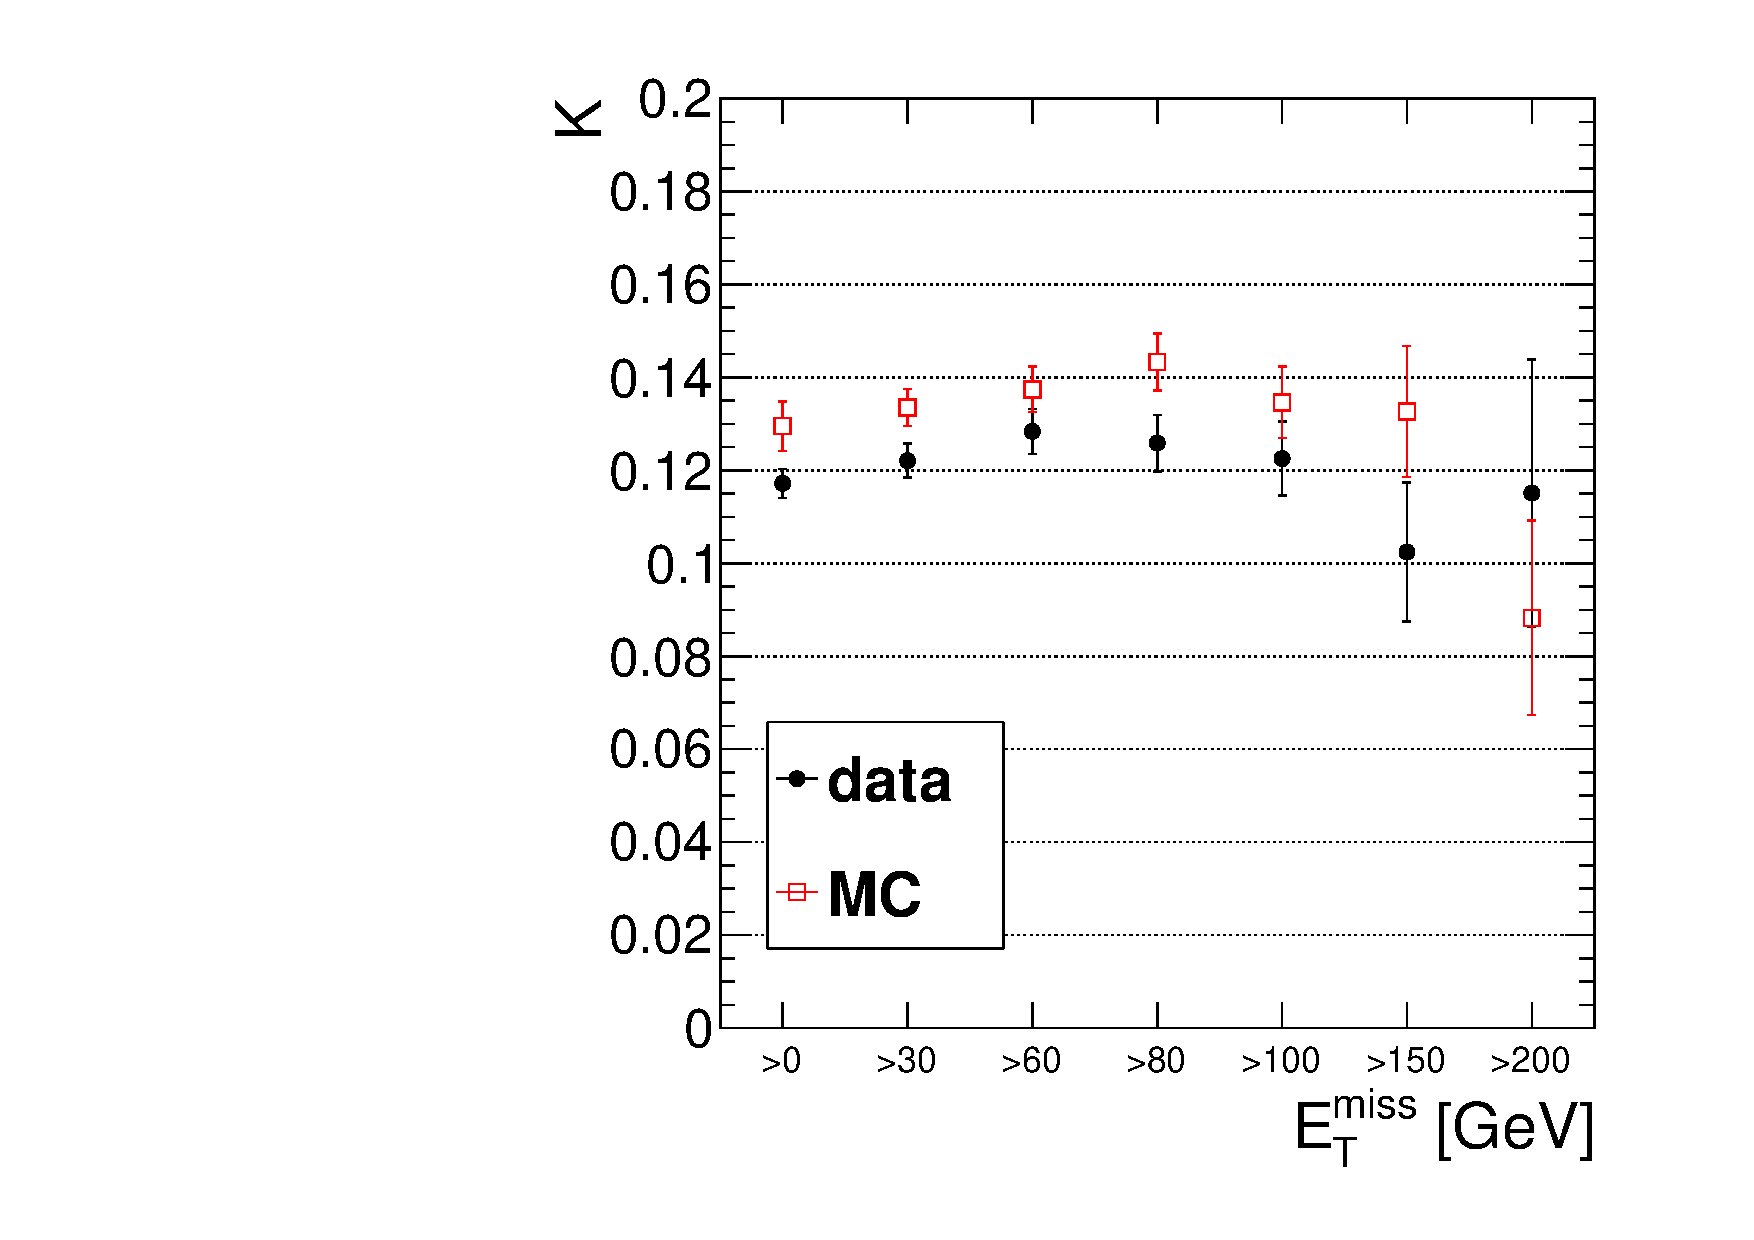
\includegraphics[width=0.4\textwidth]{plots/extractK_inclusive_bveto_19fb.pdf} &
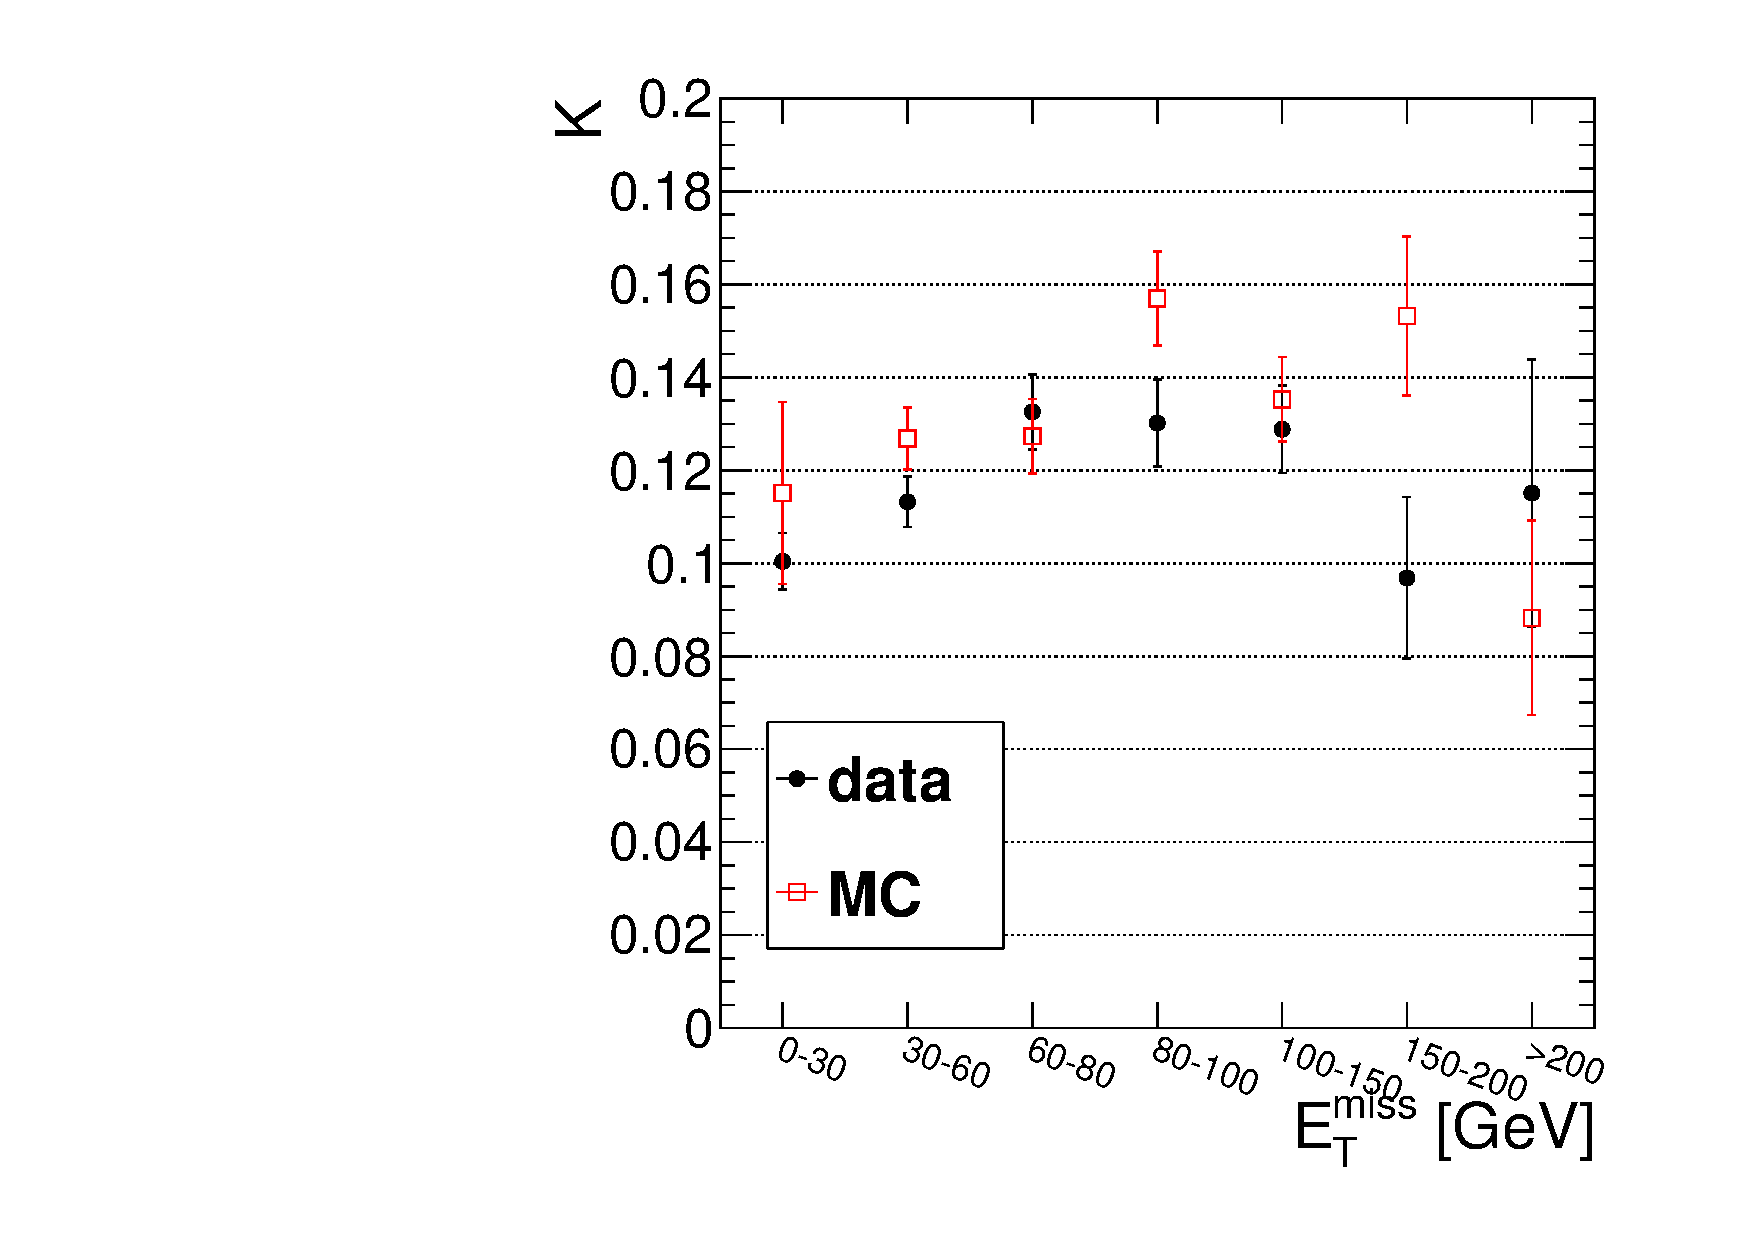
\includegraphics[width=0.4\textwidth]{plots/extractK_exclusive_bveto_19fb.pdf} \\
\end{tabular}
\caption{
The efficiency for e$\mu$ events to satisfy the dilepton mass requirement, $K$, in data and simulation for inclusive \MET\ intervals (left) and
exclusive \MET\ intervals (right) for the targeted analysis, including the b-veto. 
Based on this we chose $K=0.13\pm0.02$ for the \MET\ regions up to \MET\ $>$ 100 GeV.
For higher \MET\ regions we chose $K=0.13\pm0.07$.
%{\bf FIXME plots made with 10\% of \zjets\ MC statistics, to be remade with full statistics}
\label{fig:K_targeted}
}
\begin{comment}

Using selection : (((((leptype==2)&&(csc==0 && hbhe==1 && hcallaser==1 && ecaltp==1 && trkfail==1 && eebadsc==1 && hbhenew==1))&&(isdata==0 || (run<197556 || run>198913)))&&(njets>=2))&&(lep1.pt()>20 && lep2.pt()>20))&&(nbcsvm==0)
Using weight    : vtxweight * weight
OF entries (total)  12006
OF entries (Z mass) 1407
K                   0.117191
Warning in <TROOT::Append>: Replacing existing TH1: htot (Potential memory leak).
Warning in <TROOT::Append>: Replacing existing TH1: hZ (Potential memory leak).

--------------------------------------------------------------
pfmet>0   && pfmet<30

data  : 
total : 2719
Z     : 273
K     : 0.10 +/- 0.006

MC    : 
total : 131.974
Z     : 15.1946
K     : 0.12 +/- 0.020
--------------------------------------------------------------


--------------------------------------------------------------
pfmet>30  && pfmet<60

data  : 
total : 3842
Z     : 435
K     : 0.11 +/- 0.005

MC    : 
total : 172.956
Z     : 21.9369
K     : 0.13 +/- 0.007
--------------------------------------------------------------


--------------------------------------------------------------
pfmet>60  && pfmet<80

data  : 
total : 2029
Z     : 269
K     : 0.13 +/- 0.008

MC    : 
total : 109.789
Z     : 13.9792
K     : 0.13 +/- 0.008
--------------------------------------------------------------


--------------------------------------------------------------
pfmet>80  && pfmet<100

data  : 
total : 1490
Z     : 194
K     : 0.13 +/- 0.009

MC    : 
total : 73.3643
Z     : 11.5154
K     : 0.16 +/- 0.010
--------------------------------------------------------------


--------------------------------------------------------------
pfmet>100 && pfmet<150

data  : 
total : 1467
Z     : 189
K     : 0.13 +/- 0.009

MC    : 
total : 86.7947
Z     : 11.742
K     : 0.14 +/- 0.009
--------------------------------------------------------------


--------------------------------------------------------------
pfmet>150 && pfmet<200

data  : 
total : 320
Z     : 31
K     : 0.10 +/- 0.017

MC    : 
total : 19.4473
Z     : 2.97965
K     : 0.15 +/- 0.017
--------------------------------------------------------------


--------------------------------------------------------------
pfmet>200

data  : 
total : 139
Z     : 16
K     : 0.12 +/- 0.029

MC    : 
total : 8.99801
Z     : 0.794136
K     : 0.09 +/- 0.021
--------------------------------------------------------------

Warning in <TROOT::Append>: Replacing existing TH1: hdummy (Potential memory leak).
Info in <TCanvas::Print>: pdf file ../plots/extractK_exclusive_bveto.pdf has been created
root [3] extractK(false,true,true)
Using selection : (((((leptype==2)&&(csc==0 && hbhe==1 && hcallaser==1 && ecaltp==1 && trkfail==1 && eebadsc==1 && hbhenew==1))&&(isdata==0 || (run<197556 || run>198913)))&&(njets>=2))&&(lep1.pt()>20 && lep2.pt()>20))&&(nbcsvm==0)
Using weight    : vtxweight * weight
OF entries (total)  12006
OF entries (Z mass) 1407
K                   0.117191
Warning in <TROOT::Append>: Replacing existing TH1: htot (Potential memory leak).
Warning in <TROOT::Append>: Replacing existing TH1: hZ (Potential memory leak).

--------------------------------------------------------------
pfmet>0

data  : 
total : 12006
Z     : 1407
K     : 0.12 +/- 0.003

MC    : 
total : 603.333
Z     : 78.1422
K     : 0.13 +/- 0.005
--------------------------------------------------------------


--------------------------------------------------------------
pfmet>30

data  : 
total : 9287
Z     : 1134
K     : 0.12 +/- 0.004

MC    : 
total : 471.396
Z     : 62.9476
K     : 0.13 +/- 0.004
--------------------------------------------------------------


--------------------------------------------------------------
pfmet>60

data  : 
total : 5445
Z     : 699
K     : 0.13 +/- 0.005

MC    : 
total : 298.41
Z     : 41.0107
K     : 0.14 +/- 0.005
--------------------------------------------------------------


--------------------------------------------------------------
pfmet>80

data  : 
total : 3416
Z     : 430
K     : 0.13 +/- 0.006

MC    : 
total : 188.602
Z     : 27.0313
K     : 0.14 +/- 0.006
--------------------------------------------------------------


--------------------------------------------------------------
pfmet>100

data  : 
total : 1926
Z     : 236
K     : 0.12 +/- 0.008

MC    : 
total : 115.24
Z     : 15.5158
K     : 0.13 +/- 0.008
--------------------------------------------------------------


--------------------------------------------------------------
pfmet>150

data  : 
total : 459
Z     : 47
K     : 0.10 +/- 0.015

MC    : 
total : 28.4454
Z     : 3.77378
K     : 0.13 +/- 0.014
--------------------------------------------------------------


--------------------------------------------------------------
pfmet>200

data  : 
total : 139
Z     : 16
K     : 0.12 +/- 0.029

MC    : 
total : 8.99801
Z     : 0.794136
K     : 0.09 +/- 0.021
--------------------------------------------------------------

\end{comment}

\end{center}
\end{figure}


\begin{comment}

\begin{figure}[!hb]
\begin{center}
\begin{tabular}{cc}
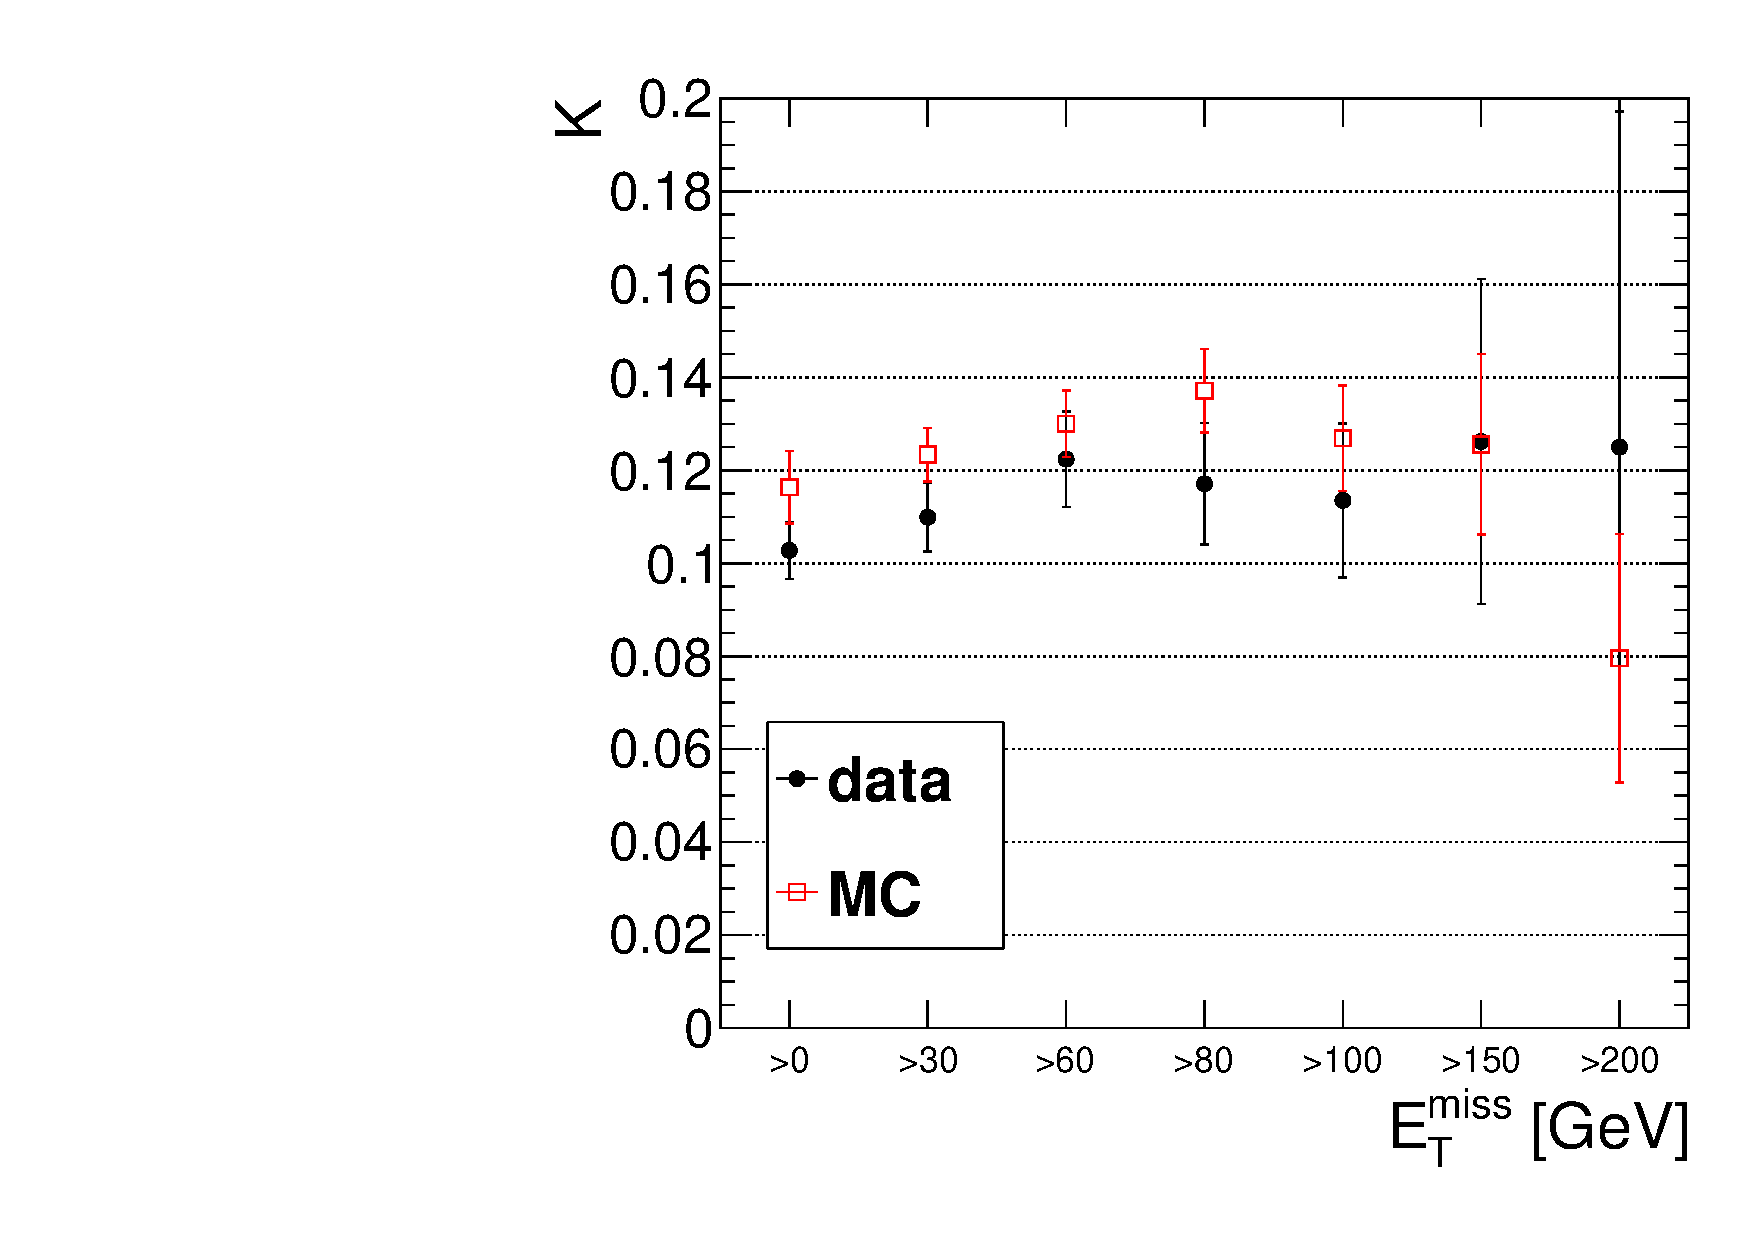
\includegraphics[width=0.4\textwidth]{plots/extractK_inclusive_bvetoLoose_92fb.pdf} &
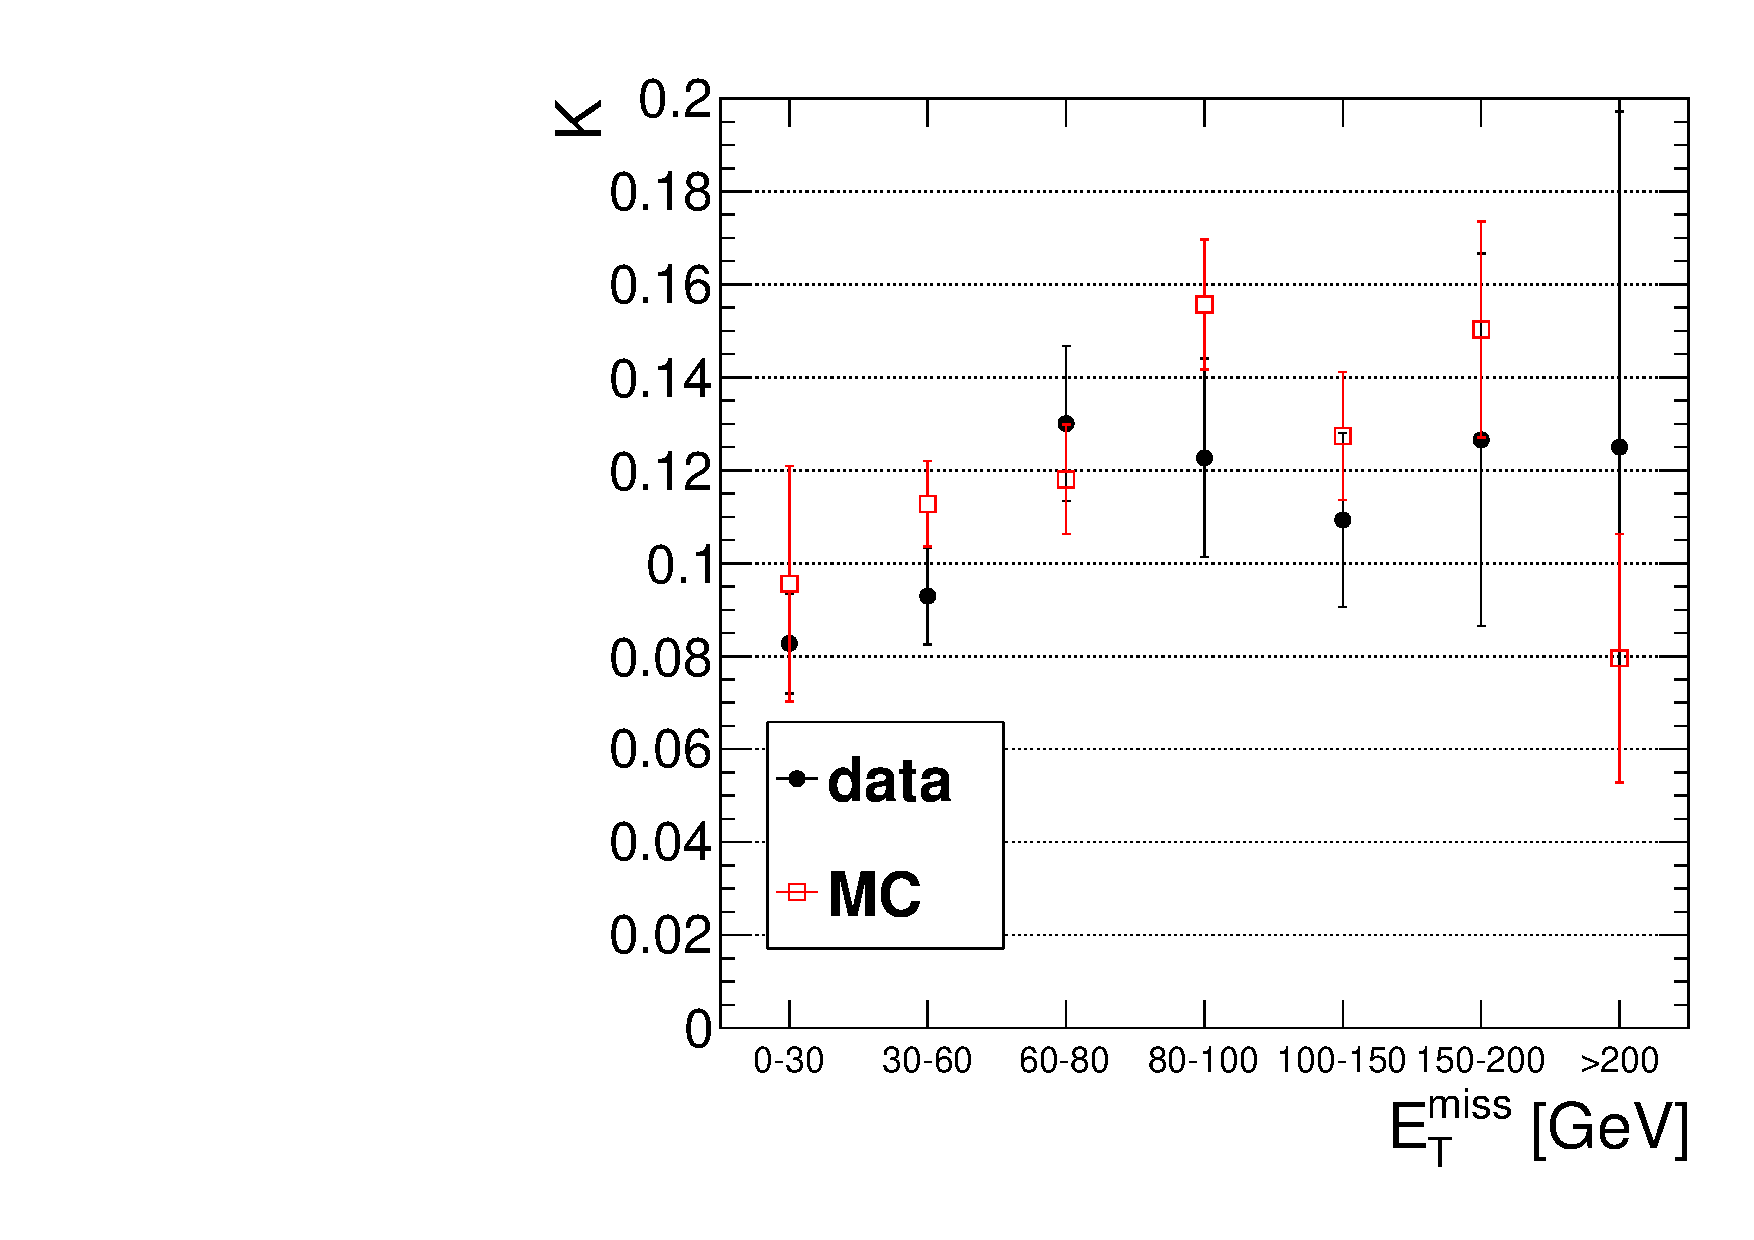
\includegraphics[width=0.4\textwidth]{plots/extractK_exclusive_bvetoLoose_92fb.pdf} \\
\end{tabular}
\caption{
The efficiency for e$\mu$ events to satisfy the dilepton mass requirement, $K$, in data and simulation for inclusive \MET\ intervals (left) and
exclusive \MET\ intervals (right) for the targeted analysis, including the b-veto. 
%{\bf FIXME plots made with 10\% of \zjets\ MC statistics, to be remade with full statistics}
\label{fig:K_targeted}}


root [2] extractK(true,false,true)
Using selection : (((((leptype==2)&&(csc==0 && hbhe==1 && hcallaser==1 && ecaltp==1 && trkfail==1 && eebadsc==1 && hbhenew==1))&&(isdata==0 || (run<197556 || run>198913)))&&(njets>=2))&&(lep1.pt()>20 && lep2.pt()>20))&&(nbcsvl==0)
Using weight    : vtxweight * weight
OF entries (total)  2715
OF entries (Z mass) 279
K                   0.102762
Warning in <TStreamerInfo::Compile>: Counter fNClusterRange should not be skipped from class TTree
Info in <TCanvas::MakeDefCanvas>:  created default TCanvas with name c1

--------------------------------------------------------------
pfmet>0   && pfmet<30

data  : 
total : 713
Z     : 59
K     : 0.08 +/- 0.011

MC    : 
total : 74.2549
Z     : 7.09789
K     : 0.10 +/- 0.025
--------------------------------------------------------------


--------------------------------------------------------------
pfmet>30  && pfmet<60

data  : 
total : 850
Z     : 79
K     : 0.09 +/- 0.010

MC    : 
total : 84.6973
Z     : 9.55105
K     : 0.11 +/- 0.009
--------------------------------------------------------------


--------------------------------------------------------------
pfmet>60  && pfmet<80

data  : 
total : 469
Z     : 61
K     : 0.13 +/- 0.017

MC    : 
total : 50.1496
Z     : 5.92081
K     : 0.12 +/- 0.012
--------------------------------------------------------------


--------------------------------------------------------------
pfmet>80  && pfmet<100

data  : 
total : 269
Z     : 33
K     : 0.12 +/- 0.021

MC    : 
total : 30.0547
Z     : 4.67993
K     : 0.16 +/- 0.014
--------------------------------------------------------------


--------------------------------------------------------------
pfmet>100 && pfmet<150

data  : 
total : 311
Z     : 34
K     : 0.11 +/- 0.019

MC    : 
total : 39.4475
Z     : 5.02593
K     : 0.13 +/- 0.014
--------------------------------------------------------------


--------------------------------------------------------------
pfmet>150 && pfmet<200

data  : 
total : 79
Z     : 10
K     : 0.13 +/- 0.040

MC    : 
total : 9.96228
Z     : 1.4975
K     : 0.15 +/- 0.023
--------------------------------------------------------------


--------------------------------------------------------------
pfmet>200

data  : 
total : 24
Z     : 3
K     : 0.12 +/- 0.072

MC    : 
total : 5.3503
Z     : 0.425719
K     : 0.08 +/- 0.027
--------------------------------------------------------------

root [3] Info in <TCanvas::Print>: pdf file /Users/benhoob/tas/ZMet2012/plots/extractK_exclusive_bvetoLoose_92fb.pdf has been created

root [3] 
root [3] extractK(false,false,true)
Using selection : (((((leptype==2)&&(csc==0 && hbhe==1 && hcallaser==1 && ecaltp==1 && trkfail==1 && eebadsc==1 && hbhenew==1))&&(isdata==0 || (run<197556 || run>198913)))&&(njets>=2))&&(lep1.pt()>20 && lep2.pt()>20))&&(nbcsvl==0)
Using weight    : vtxweight * weight
OF entries (total)  2715
OF entries (Z mass) 279
K                   0.102762
Warning in <TROOT::Append>: Replacing existing TH1: htot (Potential memory leak).
Warning in <TROOT::Append>: Replacing existing TH1: hZ (Potential memory leak).

--------------------------------------------------------------
pfmet>0

data  : 
total : 2715
Z     : 279
K     : 0.10 +/- 0.006

MC    : 
total : 293.912
Z     : 34.199
K     : 0.12 +/- 0.008
--------------------------------------------------------------


--------------------------------------------------------------
pfmet>30

data  : 
total : 2002
Z     : 220
K     : 0.11 +/- 0.007

MC    : 
total : 219.661
Z     : 27.101
K     : 0.12 +/- 0.006
--------------------------------------------------------------


--------------------------------------------------------------
pfmet>60

data  : 
total : 1152
Z     : 141
K     : 0.12 +/- 0.010

MC    : 
total : 134.962
Z     : 17.5498
K     : 0.13 +/- 0.007
--------------------------------------------------------------


--------------------------------------------------------------
pfmet>80

data  : 
total : 683
Z     : 80
K     : 0.12 +/- 0.013

MC    : 
total : 84.8149
Z     : 11.629
K     : 0.14 +/- 0.009
--------------------------------------------------------------


--------------------------------------------------------------
pfmet>100

data  : 
total : 414
Z     : 47
K     : 0.11 +/- 0.017

MC    : 
total : 54.7604
Z     : 6.94915
K     : 0.13 +/- 0.011
--------------------------------------------------------------


--------------------------------------------------------------
pfmet>150

data  : 
total : 103
Z     : 13
K     : 0.13 +/- 0.035

MC    : 
total : 15.3125
Z     : 1.92322
K     : 0.13 +/- 0.019
--------------------------------------------------------------


--------------------------------------------------------------
pfmet>200

data  : 
total : 24
Z     : 3
K     : 0.12 +/- 0.072

MC    : 
total : 5.3503
Z     : 0.425719
K     : 0.08 +/- 0.027
--------------------------------------------------------------


\end{center}
\end{figure}


\end{comment}


\clearpage

\subsection{Estimating the WZ and ZZ Background with MC}
\label{sec:bkg_vz}

Backgrounds from W($\ell\nu$)Z($\ell\ell$) where the W lepton is not identified or is outside acceptance, and Z($\nu\nu$)Z($\ell\ell$),
are estimated from simulation. The MC modeling of these processes is validated by comparing the MC predictions with data in control samples
with exactly 3 leptons (WZ control sample) and exactly 4 leptons (ZZ control sample). 
The critical samples are the WZJetsTo3LNu and ZZJetsTo4L, listed in Table~\ref{tab:mcsamples}
(the WZJetsTo2L2Q, ZZJetsTo2L2Q, and ZZJetsTo2L2Nu samples are also used in this analysis but their contribution to the 3-lepton and 4-lepton
control samples is negligible).

\subsubsection{WZ Validation Studies}
\label{sec:bkg_wz}

A pure WZ sample can be selected in data with the requirements:

\begin{itemize}
\item Exactly 3 $p_T>20$~GeV leptons passing analysis identication and isolation requirements,
\item 2 of the 3 leptons must fall in the Z window 81-101 GeV,
\item \MET $>$ 50 GeV (to suppress DY).
\end{itemize}

The data and MC yields passing the above selection are in Table~\ref{tab:wz}. 
The inclusive yields (without any jet requirements) agree within 13\%, which is consistent within
the uncertainty in the CMS measured WZ cross section (17\%). A data vs. MC comparison of kinematic
distributions (jet multiplicity, \MET, Z \pt) is given in Fig.~\ref{fig:wz}. High \MET\ 
values in WZ and ZZ events arise from highly boosted W or Z bosons that decay leptonically, 
and we therefore check that the MC does a reasonable job of reproducing the \pt distributions of the 
leptonically decaying \Z. While the inclusive WZ yields are in reasonable agreement, we observe
an excess in data in events with at least 2 jets, corresponding to the jet multiplicity requirement
in our preselection. We observe 106 events in data while the MC predicts $62\pm1.5$~(stat), representing an excess of 71\%,
as indicated in Table~\ref{tab:wz2j}. 
This excess will be studied further. For the time being, based on these studies we currently assess an uncertainty of 70\% on the WZ yield.
A data vs. MC comparison of several kinematic quantities in the sample with 3 leptons and at least 2 jets can be found in App.~\ref{app:WZ}.

\begin{comment}
We note some possible contributions to this discrepancy:

\begin{itemize}

\item {\bf The following checks refer to the 5.2 fb$^{-1}$ results and will be updated.}

\item The \zjets\ contribution is under-estimated here, for 2 reasons: first, because the \zjets\
yield passing a \MET $>$ 50 GeV requirement is under-estimated in MC and second, because the fake
rate is typically under-estimated in the MC. To get a rough idea for how much the excess depends
on the \zjets\ yield, if the \zjets\ yield is doubled then the excess is reduced from 78\% to 55\%.
Also note that we are currently using 10\% of the \zjets\ MC sample and there is 1 event with a weight 
of about 5, so the plots and tables will be remade with full \zjets\ sample.

\item The \ttbar\ contribution is under-estimated here because the fake
rate is typically under-estimated in the MC. To get a rough idea for how much the excess depends
on the \ttbar\ yield, if the \ttbar\ yield is doubled then the excess is reduced from 78\% to 57\%.

\item Currently no attempt is made to reject jets from pile-up interactions, which may be responsible
for some of the excess at large \njets. To check this, we increase the jet \pt threhsold to 40 GeV, which
helps to suppress PU jets, and observe 39 events in data vs. an MC prediction of $25\pm5.2$~(stat),
decreasing the excess from 78\% to 58\%. In the future this may be improved by explicitly
requiring the jets to be consistent with originating from the signal primary vertex.

\end{itemize}
\end{comment}



\begin{table}[htb]
\begin{center}
\caption{\label{tab:wz} Data and Monte Carlo yields passing the WZ preselection. }
\begin{tabular}{lccccc}

%Loading babies at       : ../output/V00-02-00
%Using selection         : (((((((leptype==0 && (ee==1 || isdata==0))||(leptype==1 && (mm==1 || isdata==0)))||(leptype==2 && (em==1||me==1||isdata==0)))&&(csc==0 && hbhe==1 && hcallaser==1 && ecaltp==1 && trkfail==1 && eebadsc==1 && hbhenew==1))&&(lep1.pt()>20.0 && lep2.pt()>20.0))&&(nlep==3 && lep3.pt()>20.0))&&(pfmet>50))&&(dilmass>81 && dilmass<101)
%Using weight            : weight * 19.3 * trgeff * vtxweight

\hline
\hline
         Sample   &             ee   &       $\mu\mu$   &         e$\mu$   &          total  \\
\hline
%SCALING ZJETS BY 111/946
             WZ   &244.9 $\pm$ 1.6   &317.9 $\pm$ 1.8   & 17.0 $\pm$ 0.4   &579.7 $\pm$ 2.4  \\
         \zjets   &  2.5 $\pm$ 2.0   &  6.4 $\pm$ 3.9   &  0.0 $\pm$ 0.0   &  8.9 $\pm$ 4.3  \\
             ZZ   &  5.3 $\pm$ 0.0   &  7.1 $\pm$ 0.1   &  0.4 $\pm$ 0.0   & 12.8 $\pm$ 0.1  \\
         \ttbar   &  2.5 $\pm$ 1.3   &  6.7 $\pm$ 2.0   &  7.5 $\pm$ 2.1   & 16.7 $\pm$ 3.2  \\
     single top   &  0.0 $\pm$ 0.0   &  0.5 $\pm$ 0.5   &  0.0 $\pm$ 0.0   &  0.5 $\pm$ 0.5  \\
             WW   &  0.0 $\pm$ 0.0   &  0.1 $\pm$ 0.1   &  0.2 $\pm$ 0.1   &  0.3 $\pm$ 0.1  \\
            ttV   &  8.6 $\pm$ 0.4   & 10.3 $\pm$ 0.4   &  2.5 $\pm$ 0.2   & 21.5 $\pm$ 0.7  \\
            VVV   &  3.4 $\pm$ 0.1   &  4.3 $\pm$ 0.1   &  0.6 $\pm$ 0.1   &  8.3 $\pm$ 0.2  \\
\hline
      tot SM MC   &267.1 $\pm$ 2.9   &353.3 $\pm$ 4.7   & 28.2 $\pm$ 2.2   &648.6 $\pm$ 6.0  \\
\hline
           data   &            312   &            391   &             50   &            753  \\
\hline
\hline

\end{tabular}
\end{center}
\end{table}

\begin{table}[htb]
\begin{center}
\caption{\label{tab:wz2j} Data and Monte Carlo yields passing the WZ preselection and \njets\ $\geq$ 2. }
\begin{tabular}{lccccc}

%Loading babies at       : ../output/V00-02-00
%-------------------------------------
%USING SKIMMED SAMPLES WITH NJETS >= 2
%-------------------------------------

%Using selection         : ((((((((leptype==0 && (ee==1 || isdata==0))||(leptype==1 && (mm==1 || isdata==0)))||(leptype==2 && (em==1||me==1||isdata==0)))&&(csc==0 && hbhe==1 && hcallaser==1 && ecaltp==1 && trkfail==1 && eebadsc==1 && hbhenew==1))&&(lep1.pt()>20.0 && lep2.pt()>20.0))&&(nlep==3 && lep3.pt()>20.0))&&(pfmet>50))&&(dilmass>81 && dilmass<101))&&(njets>=2)
%Using weight            : weight * 19.3 * trgeff * vtxweight

\hline
\hline
         Sample   &             ee   &       $\mu\mu$   &         e$\mu$   &          total  \\
\hline
%SCALING ZJETS BY 111/946
         \ttbar   &  1.6 $\pm$ 0.9   &  3.4 $\pm$ 1.5   &  1.8 $\pm$ 1.1   &  6.9 $\pm$ 2.0  \\
         \zjets   &  1.9 $\pm$ 1.9   &  0.0 $\pm$ 0.0   &  0.0 $\pm$ 0.0   &  1.9 $\pm$ 1.9  \\
             WZ   & 40.0 $\pm$ 0.7   & 51.5 $\pm$ 0.7   &  2.7 $\pm$ 0.2   & 94.3 $\pm$ 1.0  \\
             ZZ   &  1.0 $\pm$ 0.0   &  1.4 $\pm$ 0.0   &  0.1 $\pm$ 0.0   &  2.6 $\pm$ 0.0  \\
     single top   &  0.0 $\pm$ 0.0   &  0.5 $\pm$ 0.5   &  0.0 $\pm$ 0.0   &  0.5 $\pm$ 0.5  \\
             WW   &  0.0 $\pm$ 0.0   &  0.0 $\pm$ 0.0   &  0.0 $\pm$ 0.0   &  0.0 $\pm$ 0.0  \\
            ttV   &  8.0 $\pm$ 0.4   &  9.5 $\pm$ 0.4   &  2.2 $\pm$ 0.2   & 19.6 $\pm$ 0.6  \\
            VVV   &  1.9 $\pm$ 0.1   &  2.6 $\pm$ 0.1   &  0.2 $\pm$ 0.0   &  4.6 $\pm$ 0.2  \\
\hline
      tot SM MC   & 54.4 $\pm$ 2.2   & 69.0 $\pm$ 1.8   &  6.9 $\pm$ 1.1   &130.4 $\pm$ 3.1  \\
\hline
           data   &             87   &             91   &             22   &            200  \\
\hline
\hline

\end{tabular}
\end{center}
\end{table}

\begin{figure}[tbh]
\begin{center}
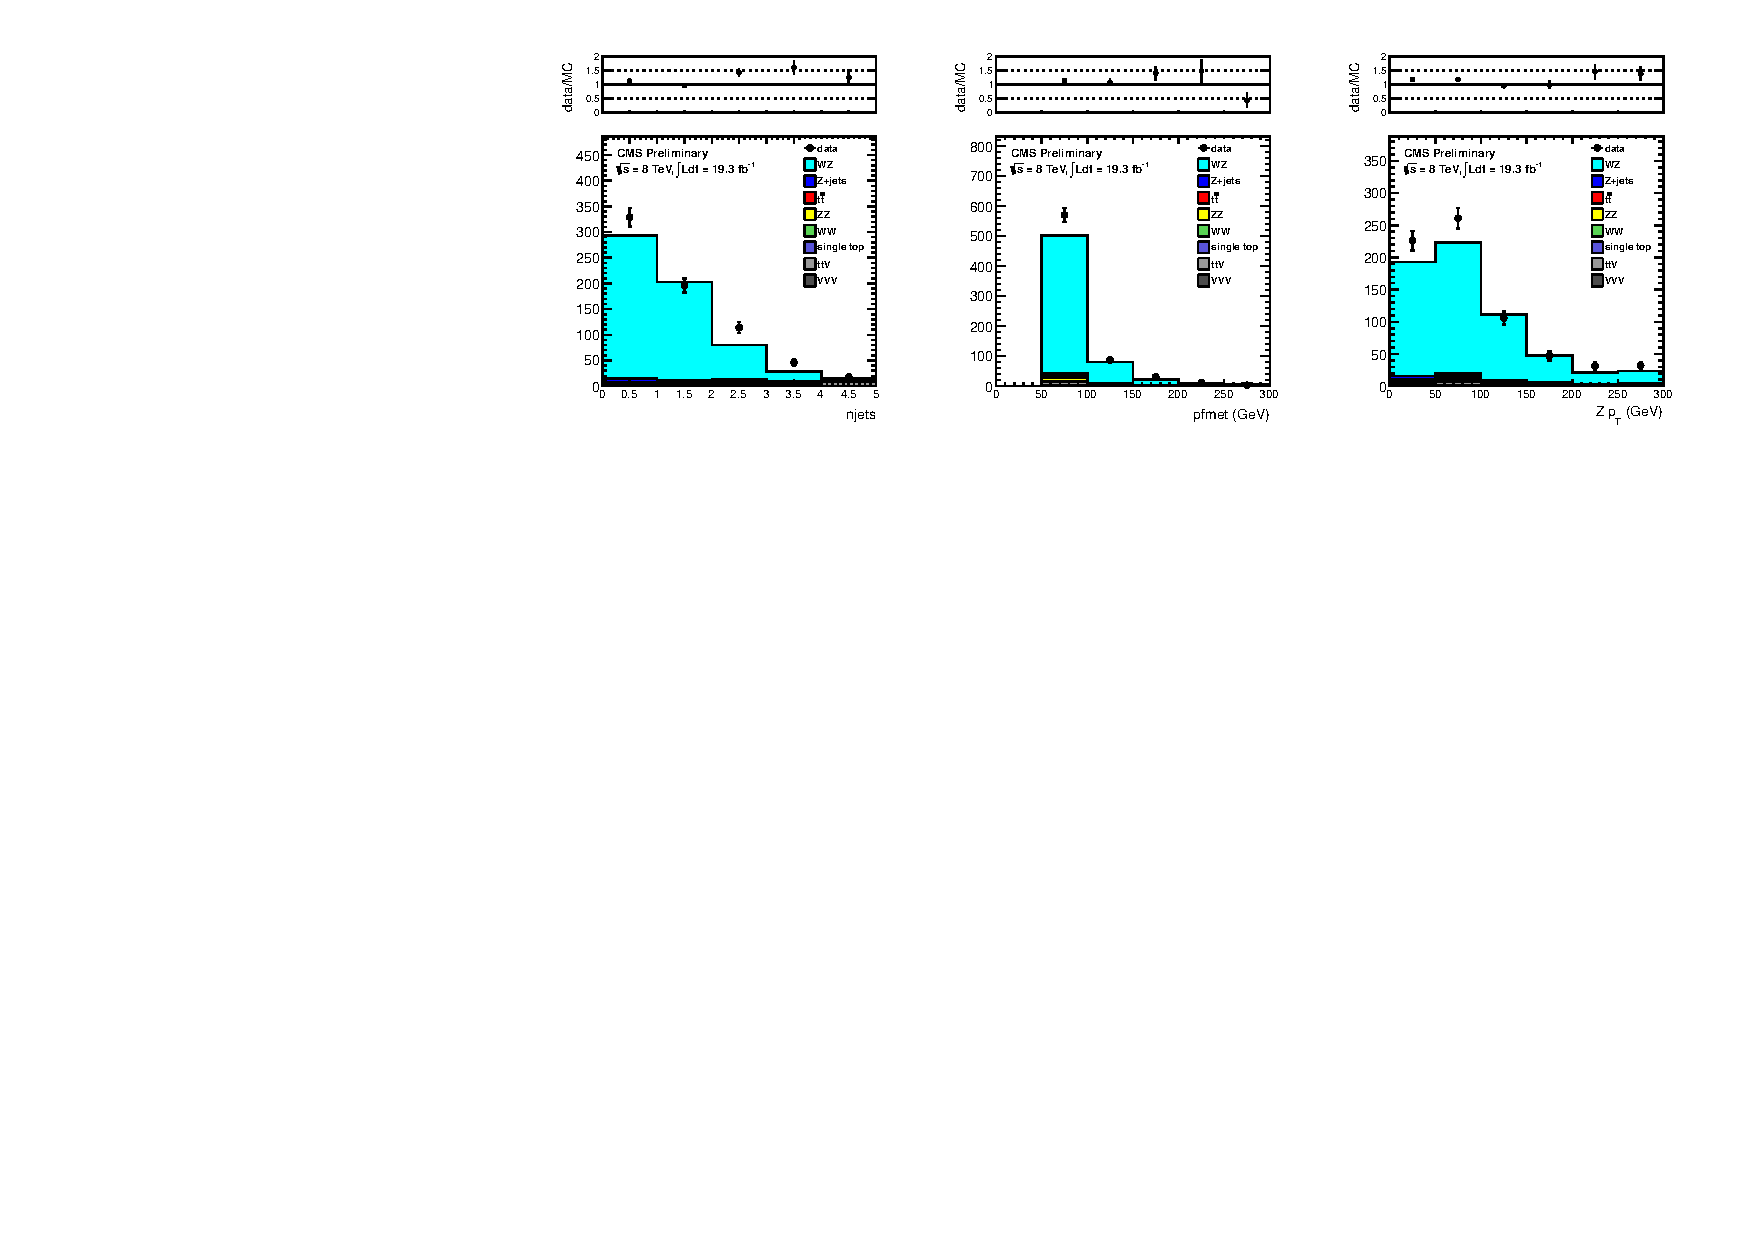
\includegraphics[width=1\linewidth]{plots/WZ_19fb.pdf}
\caption{\label{fig:wz}\protect 
Data vs. MC comparisons for the WZ selection discussed in the text for \lumi. 
The number of jets, missing transverse energy, and Z boson transverse momentum are displayed.
}
\begin{comment}
Loading babies at       : ../output/V00-02-00
Using selection         : (((((((leptype==0 && (ee==1 || isdata==0))||(leptype==1 && (mm==1 || isdata==0)))||(leptype==2 && (em==1||me==1||isdata==0)))&&(csc==0 && hbhe==1 && hcallaser==1 && ecaltp==1 && trkfail==1 && eebadsc==1 && hbhenew==1))&&(lep1.pt()>20.0 && lep2.pt()>20.0))&&(nlep==3 && lep3.pt()>20.0))&&(pfmet>50))&&(dilmass>81 && dilmass<101)
Using weight            : weight * 19.3 * trgeff * vtxweight
Plotting var njets flavor sf
compareDataMC : apply trigeff 1
MC yield VVV 7.73
MC yield ttV 18.95
MC yield single top 0.51
MC yield WW 0.09
MC yield ZZ 12.38
MC yield WZ 562.71
MC yield ttbar 9.18
SCALING ZJETS BY 111/946
MC yield zjets 8.85
MC total yield 620.39
data yield 703
Plotting var pfmet flavor sf
compareDataMC : apply trigeff 1
MC yield VVV 7.73
MC yield ttV 18.95
MC yield single top 0.51
MC yield WW 0.09
MC yield ZZ 12.38
MC yield WZ 562.72
MC yield ttbar 9.18
SCALING ZJETS BY 111/946
MC yield zjets 8.85
MC total yield 620.40
data yield 703
Plotting var dileppt flavor sf
compareDataMC : apply trigeff 1
MC yield VVV 7.73
MC yield ttV 18.95
MC yield single top 0.51
MC yield WW 0.09
MC yield ZZ 12.38
MC yield WZ 562.71
MC yield ttbar 9.18
SCALING ZJETS BY 111/946
MC yield zjets 8.85
MC total yield 620.38
data yield 703
\end{comment}

\end{center}
\end{figure}

\clearpage

\subsubsection{ZZ Validation Studies}
\label{sec:bkg_zz}

A pure ZZ sample can be selected in data with the requirements:

\begin{itemize}
\item Exactly 4 $p_T>20$~GeV leptons passing analysis identication and isolation requirements,
\item 2 of the 4 leptons must fall in the $Z$ window 81-101 GeV.
\end{itemize}

The data and MC yields passing the above selection are in Table~\ref{tab:zz}. 
In this ZZ-dominated sample we observe good agreement between the data yield and the MC prediction.
After requiring 2 jets (corresponding to the requirement in the analysis selection), we observe 4 events
in data and the MC predicts $6.6\pm0.1$ events. Due to the limited statistical precision we assign an uncertainty
fo 50\% on the ZZ yield.

\begin{table}[htb]
\begin{center}
\caption{\label{tab:zz} Data and Monte Carlo yields for the ZZ preselection. }
\begin{tabular}{lccccc}

%Loading babies at       : ../output/V00-02-00
%Using selection         : ((((((leptype==0 && (ee==1 || isdata==0))||(leptype==1 && (mm==1 || isdata==0)))||(leptype==2 && (em==1||me==1||isdata==0)))&&(csc==0 && hbhe==1 && hcallaser==1 && ecaltp==1 && trkfail==1 && eebadsc==1 && hbhenew==1))&&(lep1.pt()>20.0 && lep2.pt()>20.0))&&(nlep==4 && lep3.pt()>20.0 && lep4.pt()>20.0))&&(dilmass>81 && dilmass<101)
%Using weight            : weight * 19.3 * trgeff * vtxweight

\hline
\hline
         Sample   &             ee   &       $\mu\mu$   &         e$\mu$   &          total  \\
\hline
%SCALING ZZ BY 1.92
             ZZ   & 52.7 $\pm$ 0.2   & 73.3 $\pm$ 0.2   &  3.4 $\pm$ 0.0   &129.4 $\pm$ 0.3  \\
             WZ   &  0.1 $\pm$ 0.0   &  0.1 $\pm$ 0.0   &  0.0 $\pm$ 0.0   &  0.3 $\pm$ 0.1  \\
%SCALING ZJETS BY 111/946
         \zjets   &  0.0 $\pm$ 0.0   &  0.0 $\pm$ 0.0   &  0.0 $\pm$ 0.0   &  0.0 $\pm$ 0.0  \\
         \ttbar   &  0.0 $\pm$ 0.0   &  0.0 $\pm$ 0.0   &  0.0 $\pm$ 0.0   &  0.0 $\pm$ 0.0  \\
             WW   &  0.0 $\pm$ 0.0   &  0.0 $\pm$ 0.0   &  0.0 $\pm$ 0.0   &  0.0 $\pm$ 0.0  \\
     single top   &  0.0 $\pm$ 0.0   &  0.0 $\pm$ 0.0   &  0.0 $\pm$ 0.0   &  0.0 $\pm$ 0.0  \\
            ttV   &  1.3 $\pm$ 0.2   &  1.4 $\pm$ 0.2   &  0.3 $\pm$ 0.1   &  3.0 $\pm$ 0.2  \\
            VVV   &  0.6 $\pm$ 0.1   &  0.8 $\pm$ 0.1   &  0.0 $\pm$ 0.0   &  1.4 $\pm$ 0.1  \\
\hline
      tot SM MC   & 54.7 $\pm$ 0.3   & 75.6 $\pm$ 0.3   &  3.8 $\pm$ 0.1   &134.1 $\pm$ 0.4  \\
\hline
           data   &             56   &             80   &              5   &            141  \\
\hline
\hline

\end{tabular}
\end{center}
\end{table}

\begin{figure}[tbh]
\begin{center}
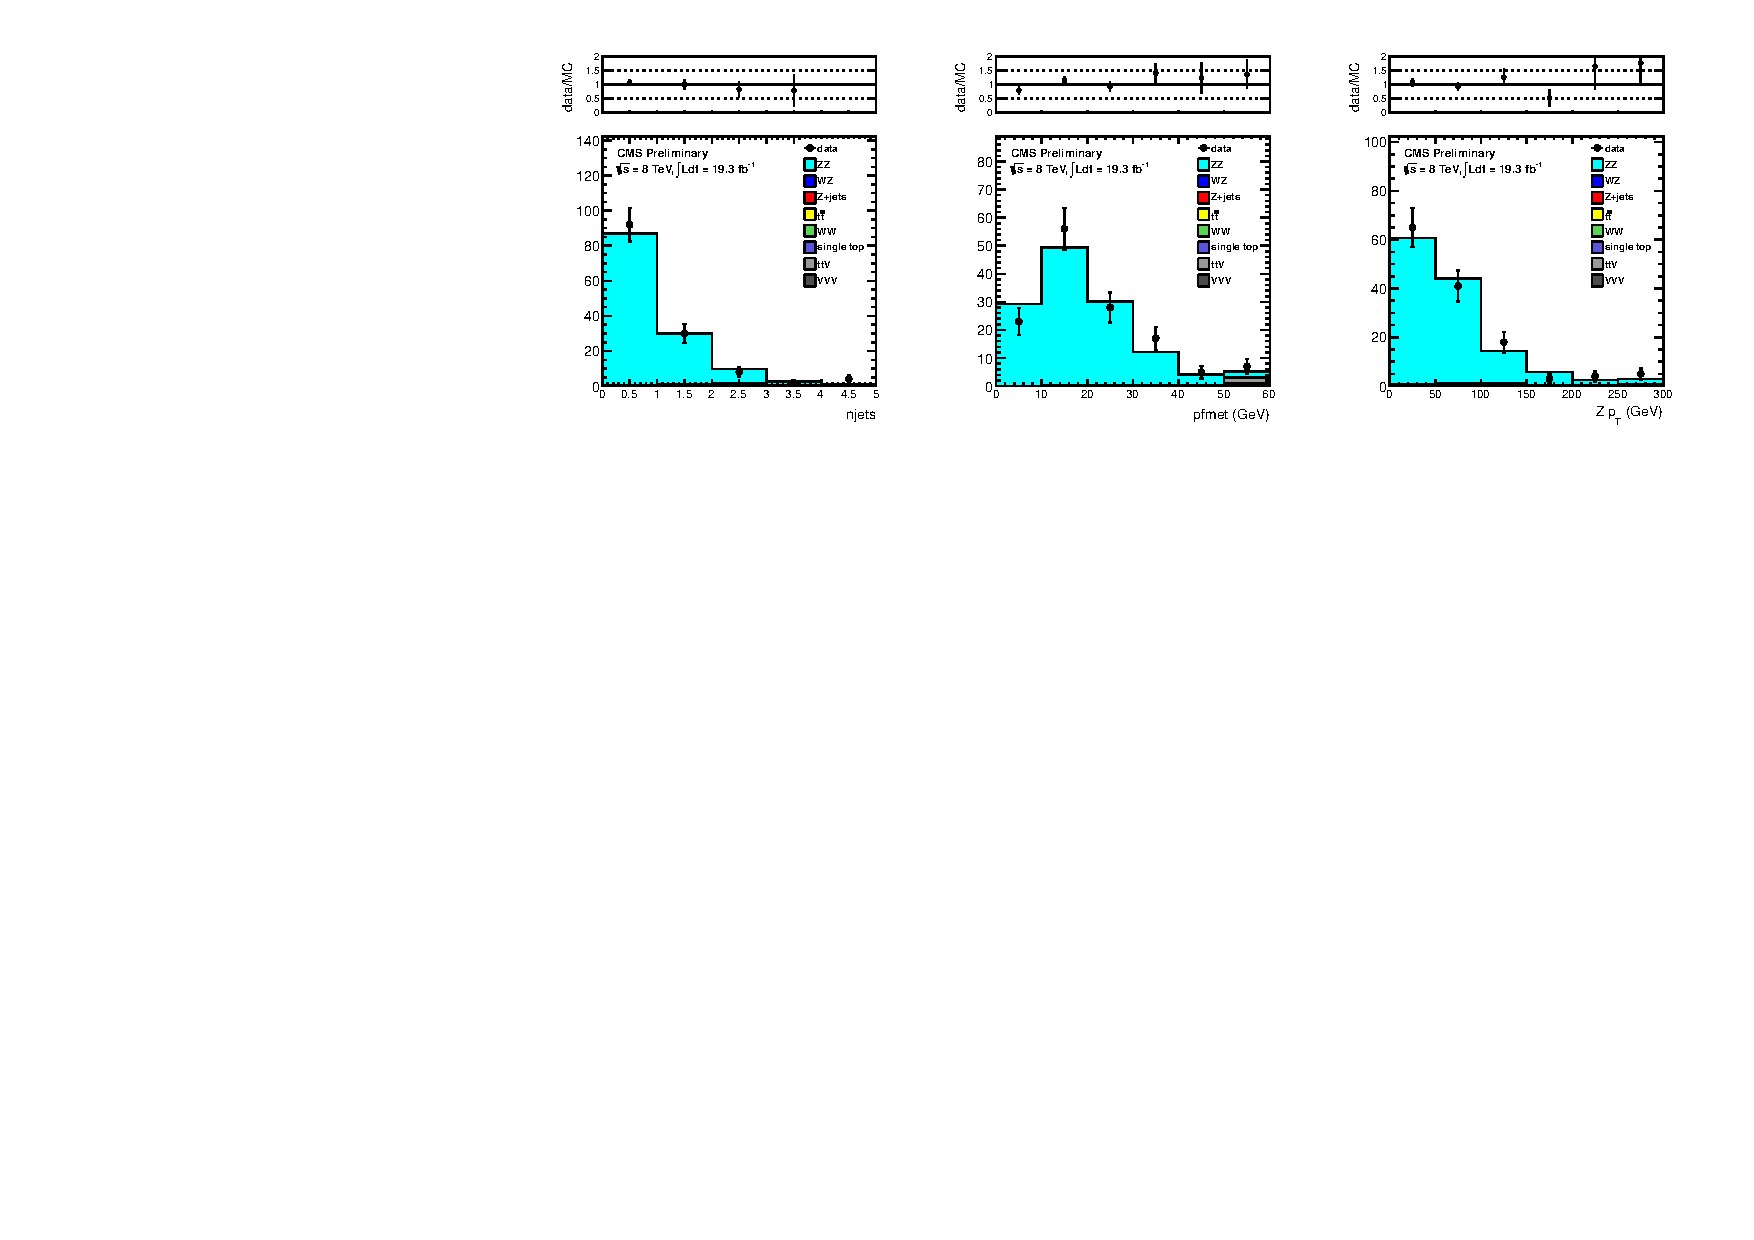
\includegraphics[width=1\linewidth]{plots/ZZ_19fb.pdf}
\caption{\label{fig:zz}\protect 
Data vs. MC comparisons for the ZZ selection discussed in the text for \lumi.
The number of jets, missing transverse energy, and Z boson transverse momentum are displayed.
}
\end{center}
\end{figure}

\begin{comment}
Loading babies at       : ../output/V00-02-00
Using selection         : ((((((leptype==0 && (ee==1 || isdata==0))||(leptype==1 && (mm==1 || isdata==0)))||(leptype==2 && (em==1||me==1||isdata==0)))&&(csc==0 && hbhe==1 && hcallaser==1 && ecaltp==1 && trkfail==1 && eebadsc==1 && hbhenew==1))&&(lep1.pt()>20.0 && lep2.pt()>20.0))&&(nlep==4 && lep3.pt()>20.0 && lep4.pt()>20.0))&&(dilmass>81 && dilmass<101)
Using weight            : weight * 19.3 * trgeff * vtxweight
Plotting var njets flavor sf
compareDataMC : apply trigeff 1

MC yield VVV 1.40
MC yield ttV 2.64
MC yield single top 0.00
MC yield WW 0.00
MC yield ttbar 0.00
SCALING ZJETS BY 111/946
MC yield zjets 0.00
MC yield WZ 0.27
SCALING ZJETS BY 1.92
MC yield ZZ 125.99
MC total yield 130.31
data yield 136
Plotting var pfmet flavor sf
compareDataMC : apply trigeff 1
MC yield VVV 1.40
MC yield ttV 2.64
MC yield single top 0.00
MC yield WW 0.00
MC yield ttbar 0.00
SCALING ZJETS BY 111/946
MC yield zjets 0.00
MC yield WZ 0.27
SCALING ZJETS BY 1.92
MC yield ZZ 126.00
MC total yield 130.32
data yield 136
Plotting var dileppt flavor sf
compareDataMC : apply trigeff 1
MC yield VVV 1.40
MC yield ttV 2.64
MC yield single top 0.00
MC yield WW 0.00
MC yield ttbar 0.00
SCALING ZJETS BY 111/946
MC yield zjets 0.00
MC yield WZ 0.27
SCALING ZJETS BY 1.92
MC yield ZZ 126.00
MC total yield 130.33
data yield 136
\end{comment}



%\subsection{Estimating the Rare SM Backgrounds with MC}
%\label{sec:bkg_raresm}

%{\bf TODO: list samples, yields in preselection region, and show \MET\ distribution}

\section{Results}
\label{sec:results}

\subsection{Background estimate from the ABCD method}
\label{sec:abcdres}

We begin by applying the ABCD method to estimate the background in the 2010 signal region.
The data yields in the four regions are summarized in Tables~\ref{tab:datayield1} and
the $y$ vs. \Ht\ distributions are displayed in Fig.~\ref{fig:abcdData1}.
The ABCD background prediction is $N_A \times N_C / N_B = 12.7 \pm 2.4$ (stat), in
agreement with the MC expectation. We also apply the ABCD' method to estimate the
background in this region, following the procedure of App.~\ref{app:abcdprime},
and find a predicted background of $12.8 \pm 2.9$ (stat), in good agreement
with the ABCD prediction.

Next, we apply the ABCD' method to predict the yields in the high \met\ and high \Ht\
signal regions. The $y$ vs. \Ht\ distributions for data are displayed in 
Fig.~\ref{fig:abcdprimedata}. The signal regions are indicated, as well as the control 
regions used to measure the $f(y)$ and $g(H_T)$ distributions. For the high \met\
signal region, we find a predicted yield of $1.0 \pm 0.3$ (stat), in reasonable
agreement with the MC prediction. For the high \Ht\ signal region, we do not find
any events in the control region used to extract $g(H_T)$ with \Ht\ $>$ 600 GeV,
and the ABCD' background estimate is therefore 0. To assess the statistical uncertainty
in this prediction, we add a single event ``by hand'' to the $g(H_T)$ distributiion
at $H_T = 600$ GeV, leading to a predicted yield of 0.6. 
{\bf NEED TO THINK ABOUT THIS. THE PREDICTION DEPENDS ON WHERE IN HT YOU PUT THIS }
{\bf SINGLE EVENT. FOR EXAMPLE, PUTTING IT AT 1000 GIVES A PREDICTION OF 1.2      }
{\bf HOPEFULLY WITH ~3X MORE STATS WE WON'T BE IN THIS SITUATION                  }
These results are summarized in Table~\ref{tab:abcdprime}.

\begin{table}[hbt]
\begin{center}
\caption{\label{tab:abcdprime} 
Summary of results of the ABCD' method, applied to the 3 signal regions. The correction
factors are given in Table~\ref{tab:cor}.
}
\begin{tabular}{lccccc}
\hline
Signal Region             &     ABCD' pred      &  correction factor  &  prediction                                  \\ 
\hline
2010 signal region        &  $12.8 \pm 2.9$     & $1.0 \pm 0.2$      & 12.8 $\pm$ 2.9 (stat) $\pm$ 2.6 (syst)        \\
high \met\ signal region  &  $1.0  \pm 0.3$     & $1.2 \pm 0.5$      &  1.2 $\pm$ 0.4 (stat) $\pm$ 0.5 (syst)        \\
high \Ht\ signal region   &  $0.0  \pm 0.6$     & $1.0 \pm 0.5$      &  0.0 $\pm$ 0.6 (stat) $\pm$ 0.3 (syst)        \\
\hline
\end{tabular}
\end{center}
\end{table}

\begin{figure}[tbh]
\begin{center}
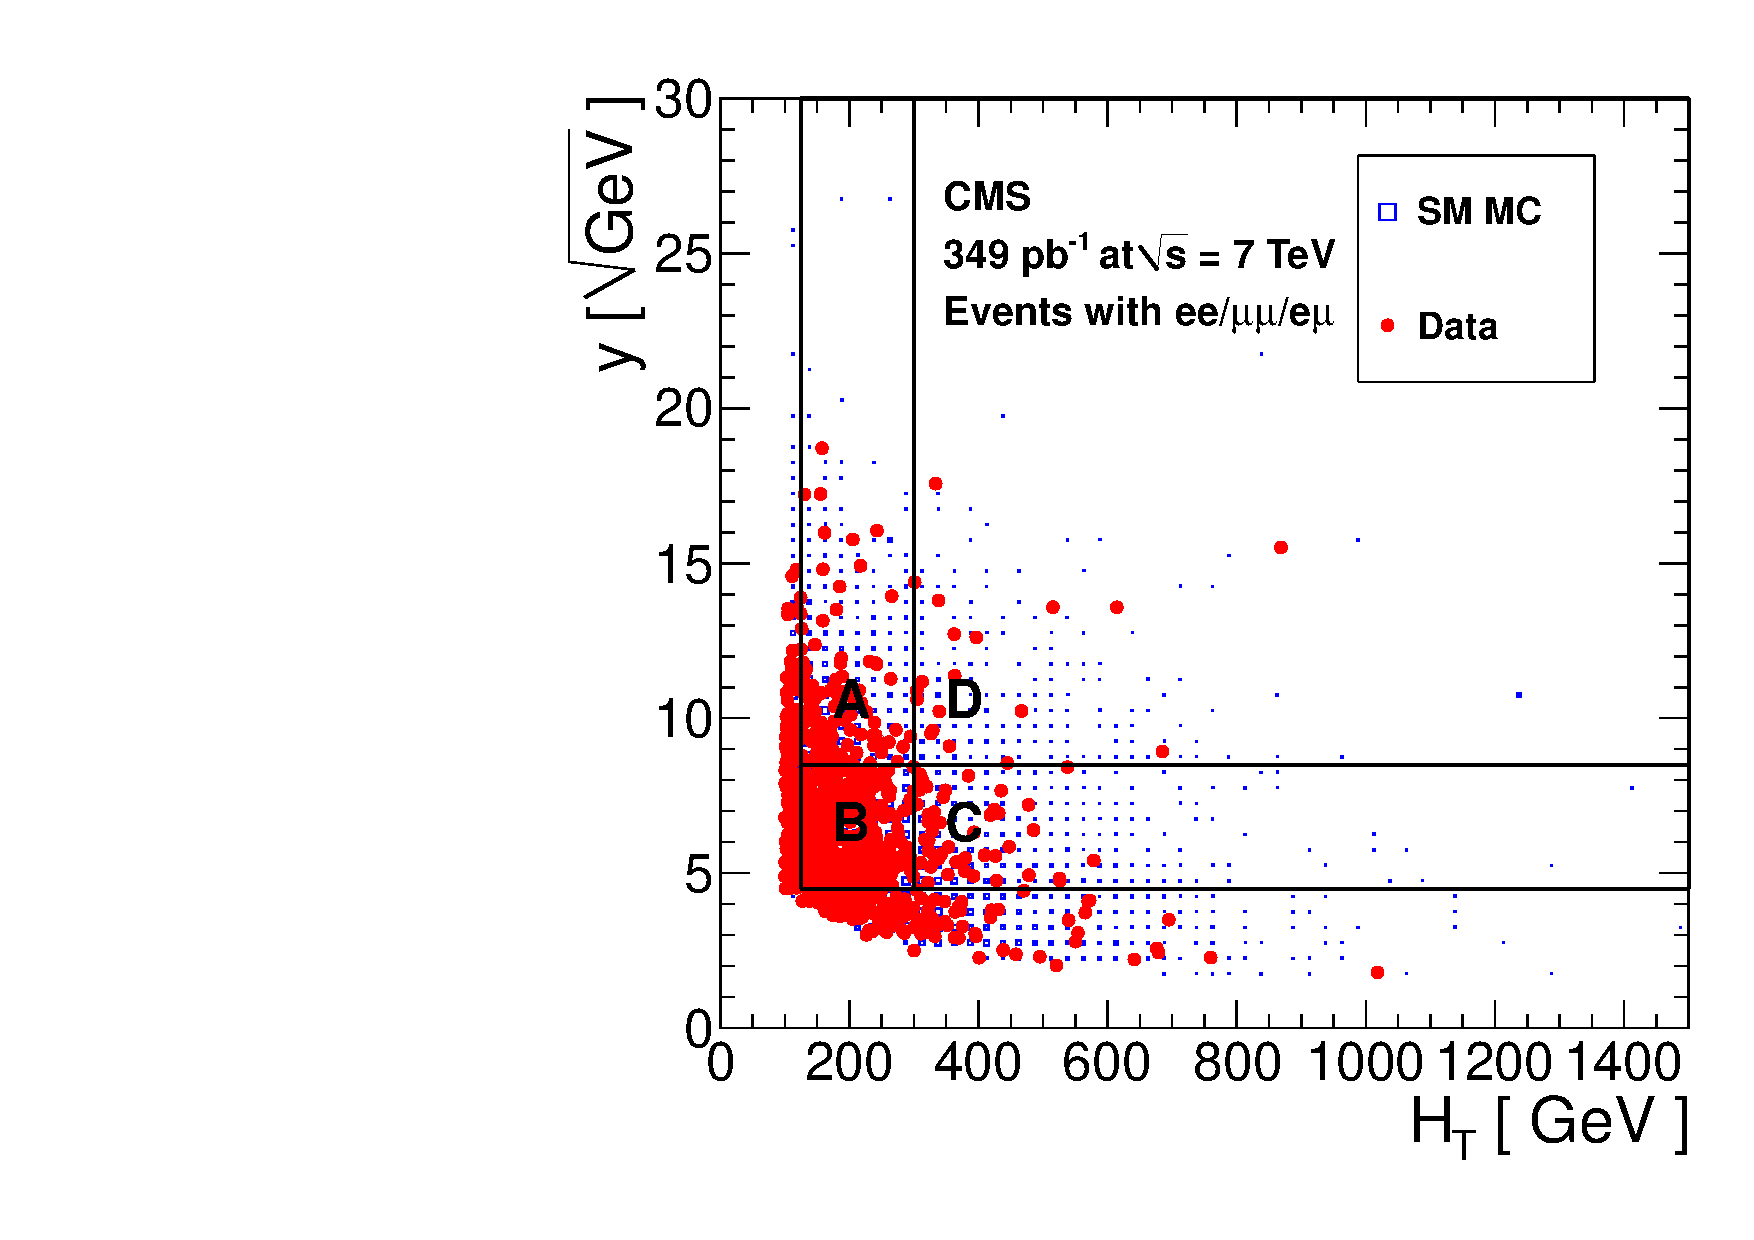
\includegraphics[width=0.6\linewidth]{plots/abcd_349pb.pdf}
\caption{\label{fig:abcdData1}\protect Distributions of $y$ 
vs. \Ht\ for SM Monte Carlo and data. The 2010 signal region boundaries are overlayed.}
\end{center}
\end{figure}

\begin{table}[hbt]
\begin{center}
\caption{\label{tab:datayield1} 
Data yields in the four
regions of Figure~\ref{fig:abcdData1} for the 2010 signal region, 
as well as the predicted yield in region D given
by $N_A \times N_C / N_B$.  The quoted uncertainty
on the prediction in data is statistical only, assuming Gaussian errors.
We also show the SM Monte Carlo expectations with statistical errors only.
}
\begin{tabular}{l||c|c|c|c||c}
\hline
           sample  &            $N_A$  &            $N_B$  &            $N_C$  &             $N_D$  &   $N_A \times N_C / N_B$ \\
\hline
            \ttll  & 63.9  $\pm$  2.0  &252.3  $\pm$  4.1  & 43.3  $\pm$  1.7  &  8.5  $\pm$  0.7  & 11.0  $\pm$  0.6        \\
           \tttau  & 18.5  $\pm$  1.1  & 55.9  $\pm$  1.9  & 10.3  $\pm$  0.8  &  3.4  $\pm$  0.5  &  3.4  $\pm$  0.4        \\
          \ttfake  &  1.0  $\pm$  0.3  &  6.6  $\pm$  0.7  &  1.1  $\pm$  0.3  &  0.4  $\pm$  0.2  &  0.2  $\pm$  0.1        \\
               DY  &  0.9  $\pm$  0.6  & 13.9  $\pm$  2.6  &  1.3  $\pm$  0.8  &  1.7  $\pm$  1.0  &  0.1  $\pm$  0.1        \\
              \WW  &  1.1  $\pm$  0.1  &  2.7  $\pm$  0.2  &  0.2  $\pm$  0.1  &  0.3  $\pm$  0.1  &  0.1  $\pm$  0.0        \\
              \WZ  &  0.1  $\pm$  0.0  &  0.6  $\pm$  0.0  &  0.1  $\pm$  0.0  &  0.0  $\pm$  0.0  &  0.0  $\pm$  0.0        \\
              \ZZ  &  0.0  $\pm$  0.0  &  0.2  $\pm$  0.0  &  0.0  $\pm$  0.0  &  0.0  $\pm$  0.0  &  0.0  $\pm$  0.0        \\
       single top  &  3.3  $\pm$  0.2  &  9.6  $\pm$  0.3  &  0.4  $\pm$  0.1  &  0.1  $\pm$  0.0  &  0.1  $\pm$  0.0        \\
           \wjets  &  1.0  $\pm$  1.0  &  2.2  $\pm$  1.1  &  0.0  $\pm$  0.0  &  0.0  $\pm$  0.0  &  0.0  $\pm$  0.0        \\
\hline
      Total SM MC  & 89.9  $\pm$  2.6  &344.0  $\pm$  5.3  & 56.6  $\pm$  2.1  & 14.5  $\pm$  1.4  & 14.8  $\pm$  0.7        \\
\hline
             data  &              110  &              381  &               44  &               19  & 12.7  $\pm$  2.4        \\
\hline
\end{tabular}
\end{center}
\end{table}


\begin{figure}[hbt]
\begin{center}
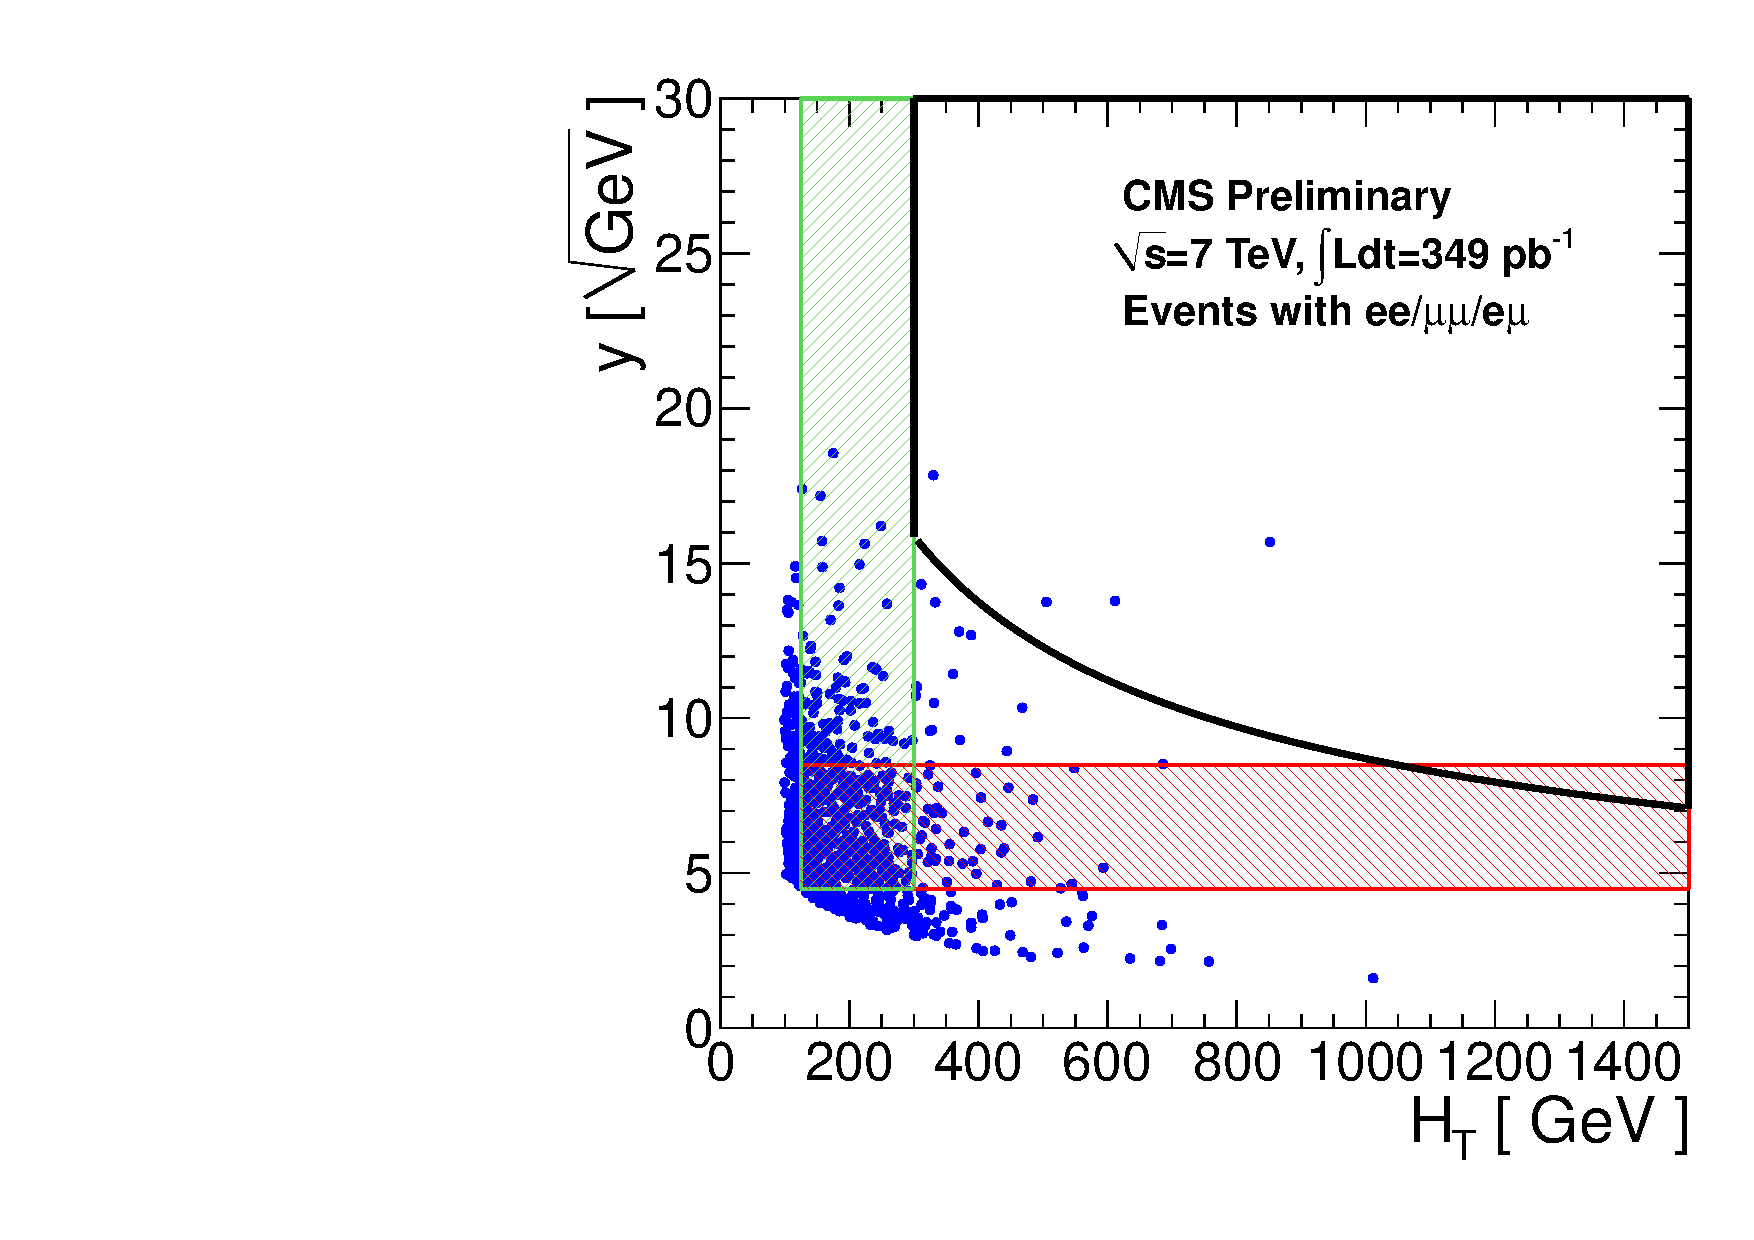
\includegraphics[width=0.48\linewidth]{plots/abcdprime_349pb_highmet.pdf}
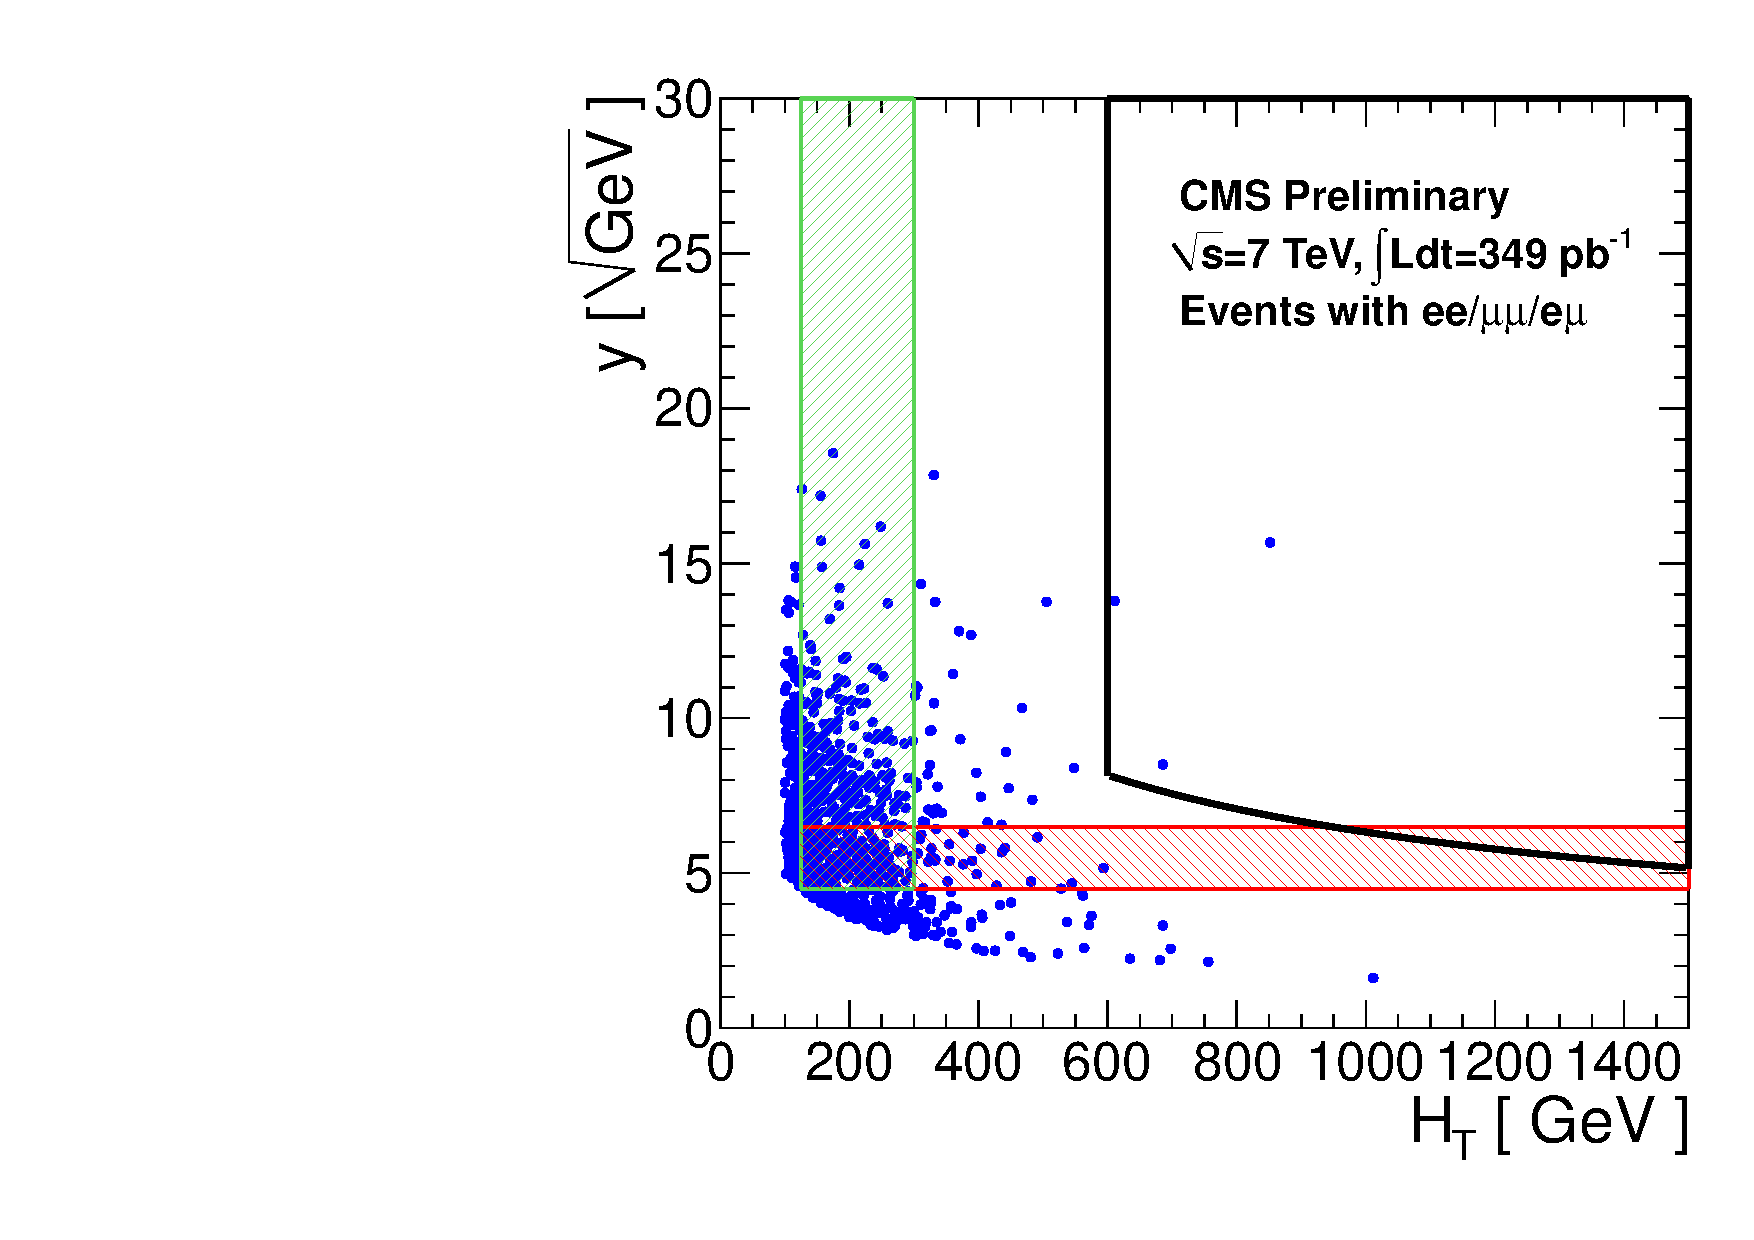
\includegraphics[width=0.48\linewidth]{plots/abcdprime_349pb_highht.pdf}
\caption{\label{fig:abcdprimedata}\protect 
Distributions of $y$ vs. \Ht\ in data. The signal regions \met\ $>$ 275 GeV, \Ht\ $>$ 300 GeV (left)
and \met\ $>$ 200 GeV, \Ht\ $>$ 600 GeV (right) are indicated with thick black lines. 
The $f(y)$ and $g(H_T)$ 
functions are measured using events in the green and red shaded areas, respectively.
}
\end{center}
\end{figure}

\subsection{Background estimate from the $P_T(\ell\ell)$ method}
\label{sec:victoryres}

We begin by extracting the value of the \met\ acceptance scaling factor $K$ from data,
for the \Ht\ control region 125--300 GeV and for the 2 signal regions \Ht\ $>$ 300 and
\Ht\ $>$ 600 GeV. The quantity $1/K$ is the efficiency for events passing preselection
and falling in the given \Ht\ range to pass the requirement \ptll\ $>$ 50 GeV.
The values of $K$ extracted from data and \ttbar\ MC are given in Table~\ref{tab:K}.
For all 3 \Ht\ regions, the value of $K$ extracted from data agrees with the 
\ttbar\ MC prediction, but for the \Ht\ $>$ 600 GeV region the statistical uncertainty
in $K$ from data is $\sim$100\%. Therefore we use the value of $K$ extracted from
data for the control region 125--300 GeV and for the signal regions \Ht\ $>$ 300;
for the \Ht\ $>$ 600 GeV region we use $K$ from \ttbar\ MC.


\begin{table}[hbt]
\begin{center}
\caption{\label{tab:K} 
Summary of the \met\ acceptance scaling factor $K$, extracted from data and \ttbar\ MC.
}
\begin{tabular}{lccccc}
\hline
region                                    &  data              &   \ttbar\ MC      \\
\hline
control region: 125 $<$ \Ht\ $<$ 300 GeV  &  1.68 $\pm$ 0.14   &   1.67 $\pm$ 0.03 \\
signal region: \Ht\ $>$ 300 GeV           &  1.45 $\pm$ 0.29   &   1.50 $\pm$ 0.06 \\
signal region: \Ht\ $>$ 600 GeV           &  1.12 $\pm$ 1.19   &   1.32 $\pm$ 0.20 \\
\hline
\end{tabular}
\end{center}
\end{table}



\begin{table}[hbt]
\begin{center}
\caption{\label{tab:victory} 
Summary of results of the dilepton $p_{T}$ template method applied to the 3 signal regions.
The quantities indicated in the table are discussed in the text.
The quoted statistical uncertainty in the prediction $N_P$ is due to
that of $N(D')$, the quoted systematic uncertainty includes that of $N(DY)$, $K$, and $K_C$.
%{\bf K and KC taken from MC, do we want to take K and/or KC from data? }
%{\bf Need to add jet/met uncertainty here}
%{\color{red} \bf CURRENTLY USING 30\% UNCERTAINTY ON K_C IN 2010 REGION, WHICH IS WHAT WE HAD LAST YEAR (NEED TO REPEAT JET/MET UNCERTAINTIES?).}
%{\color{red} \bf FOR HIGH Y/HIGH HT REGION, TAKING SYST UNCERTAINTY ON KC FROM MC STATS, WHICH IS PROBABLY DOMINANT}
}
\begin{tabular}{lccccc}
\hline
Signal Region               &  $N(D')$   &   $N(DY)$         &          $K$   &   $K_C$        & $N_P$                                   \\ 
\hline
2010 signal region (UPDATE) &       9    &   0.8 $\pm$ 0.4   & 1.5 $\pm$ 0.3  & 1.4 $\pm$ 0.4  & 16.7 $\pm$ 6.1 (stat) $\pm$ 5.9 (syst)  \\
high \met\ signal region    &       3    &   0.5 $\pm$ 0.3   & 1.5 $\pm$ 0.3  & 1.5 $\pm$ 0.5  & 5.4 $\pm$ 3.8 (stat) $\pm$ 2.2 (syst)   \\
high \Ht\ signal region     &       1    &   0.0 $\pm$ 0.0   & 1.3 $\pm$ 0.2  & 1.3 $\pm$ 0.4  & 1.7 $\pm$ 1.7 (stat) $\pm$ 0.6 (syst)   \\
\hline
\end{tabular}
\end{center}
\end{table}

For each signal region D, we count the number of events falling in the region D', which is defined
using the same requirements as D but switching the $y$ requirement to a $\ptll/\sqrt{H_T}$ requirement (2010 signal region)
or switching the \met\ requirement to a \ptll\ requirement (high \met\ and high \Ht\ signal regions).
We subtract off the expected DY contribution using the data-driven $R_{out/in}$ technique, using $R_{out/in} = 0.13 \pm 0.07$.
%{\color{red} \bf add plot justifying this value}. 
We then scale this yield by 2 corrections factors:
$K$, the \met\ acceptance correction factor, and $K_C$, the correction factor determined in Sec.~\ref{sec:datadriven}.
Our final prediction $N_P$ is given by:

\begin{center}
$ N_P = (N(D')-N(DY)) \times K \times K_C$,
\end{center}

as summarized in Table~\ref{tab:victory}, and displayed in Figs.~\ref{fig:vic1}-\ref{fig:vic3}.
We also perform the \ptll\ method in the \Ht\ sideband region 125--300~GeV, as a validation of the technique in a high statistics
sample which is expected to be dominated by background. The results are summarized in Table~\ref{tab:victorycontrol}
and displayed in Fig.~\ref{fig:victorycontrol}.
The prediction is extractedd for the requirement $y > 8.5$~GeV$^{1/2}$ corresponding to the 2010 signal region, as well as
for \met\ $>$ 200 GeV corresponding to the high \Ht\ signal region. In both cases, we observe good agreement between
the predicted and observed yields. 


\begin{table}[hbt]
\begin{center}
\caption{\label{tab:victorycontrol} 
Summary of results of the dilepton $p_{T}$ template method applied to the \Ht\ sideband control region 125--300 GeV.
The quantities indicated in the table are discussed in the text.
The quoted statistical uncertainty in the prediction $N_P$ is due to
that of $N(D')$, the quoted systematic uncertainty includes that of $N(DY)$ and $K_C$.
The predictions are compare with the observed yield $N_O$.
}
\begin{tabular}{lcccccc}
\hline
Control Region                                   &  $N(D')$   &   $N(DY)$        &  $K$          &   $K_C$          & $N_P$                                     & $N_O$ \\ 
\hline                                           
125 $<$ \Ht\ $<$ 300~GeV, $y >$ 8.5~GeV$^{1/2}$  &     54      &  2.6 $\pm$ 1.2   & 1.7 $\pm$ 0.1 & 1.4 $\pm$ 0.1    & 120.9 $\pm$ 17.3 (stat) $\pm$ 13.6 (syst) & 110   \\
125 $<$ \Ht\ $<$ 300~GeV, \met\ $>$ 200 GeV     &      4      &  1.0 $\pm$ 0.5   & 1.7 $\pm$ 0.1 & 1.3 $\pm$ 0.2    &   6.5 $\pm$  4.4 (stat) $\pm$  1.6 (syst) &   6   \\
\hline
\end{tabular}
\end{center}
\end{table}



\begin{figure}[hbt]
\begin{center}
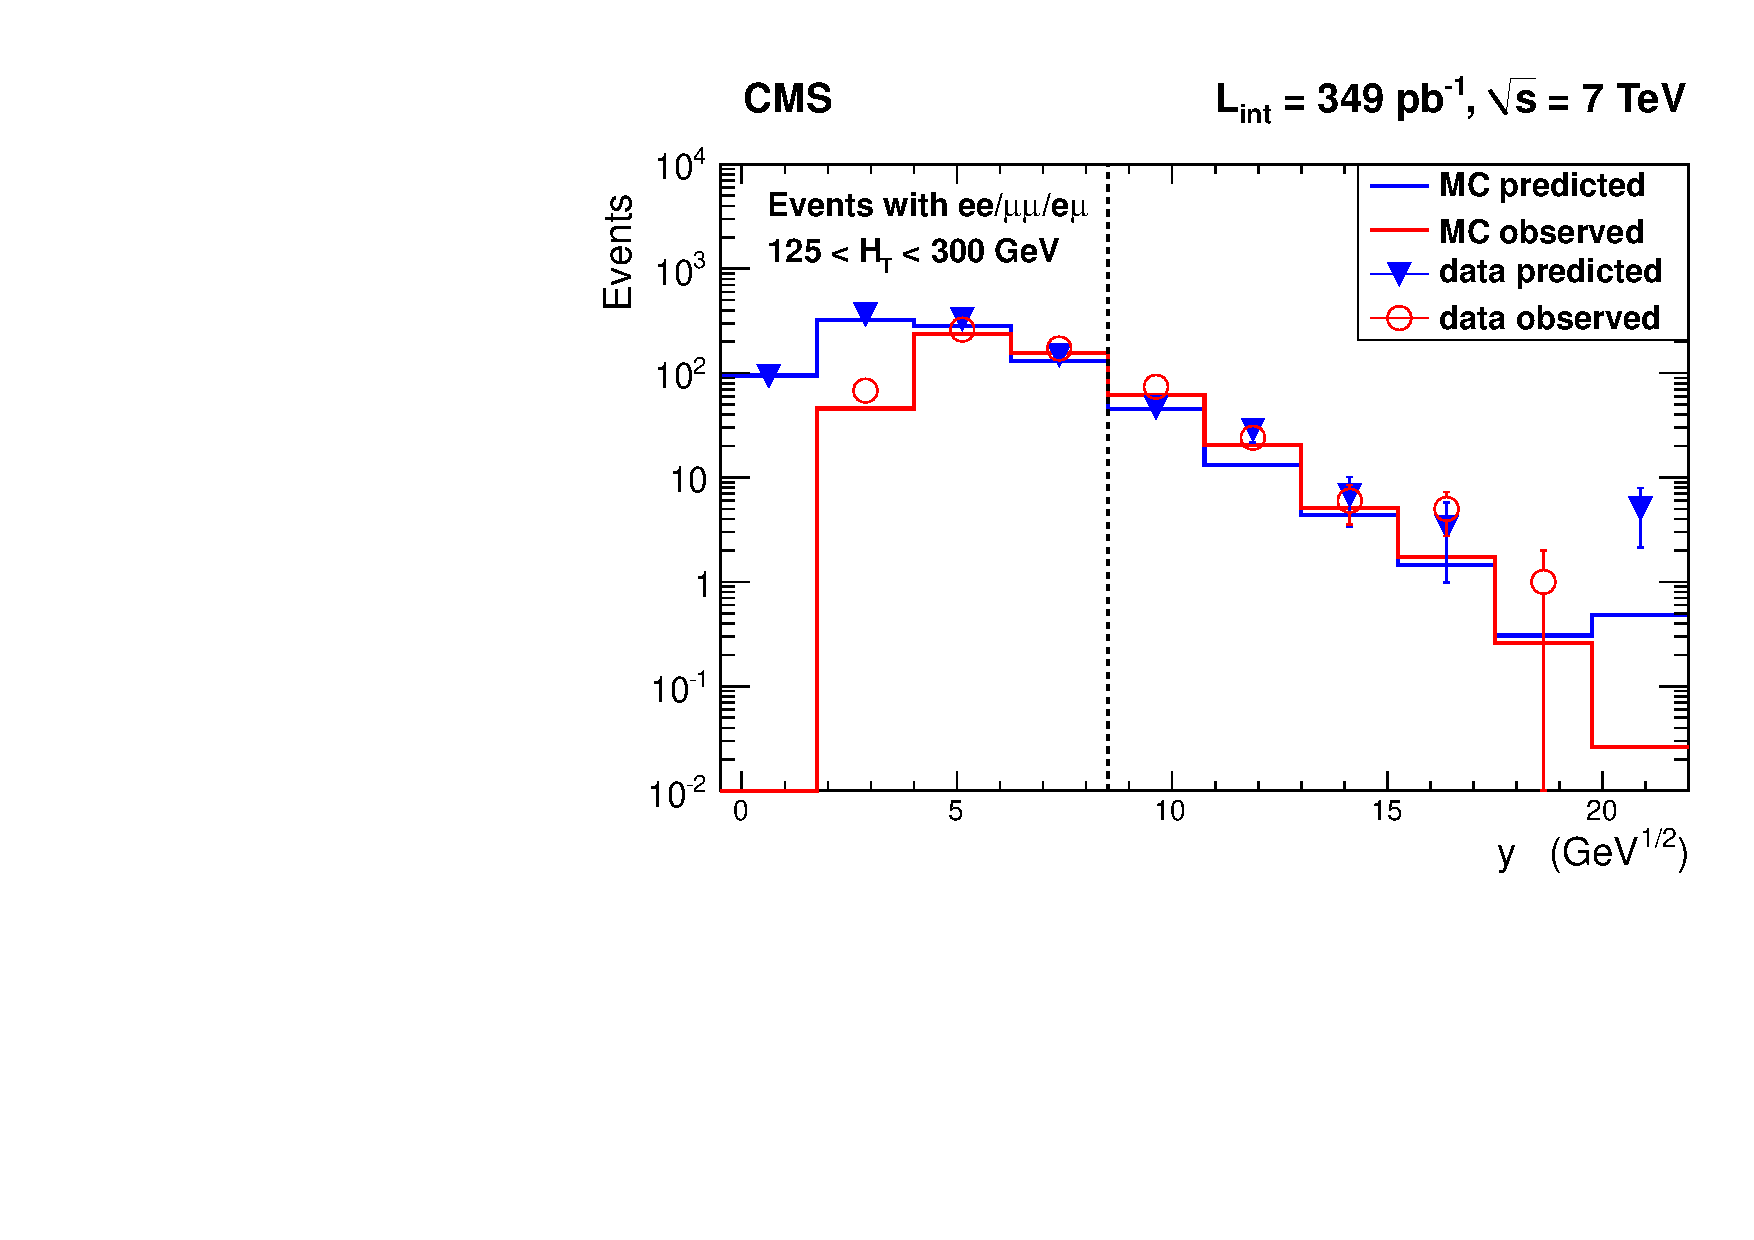
\includegraphics[width=0.48\linewidth]{plots/victory_y_control_349pb.pdf}
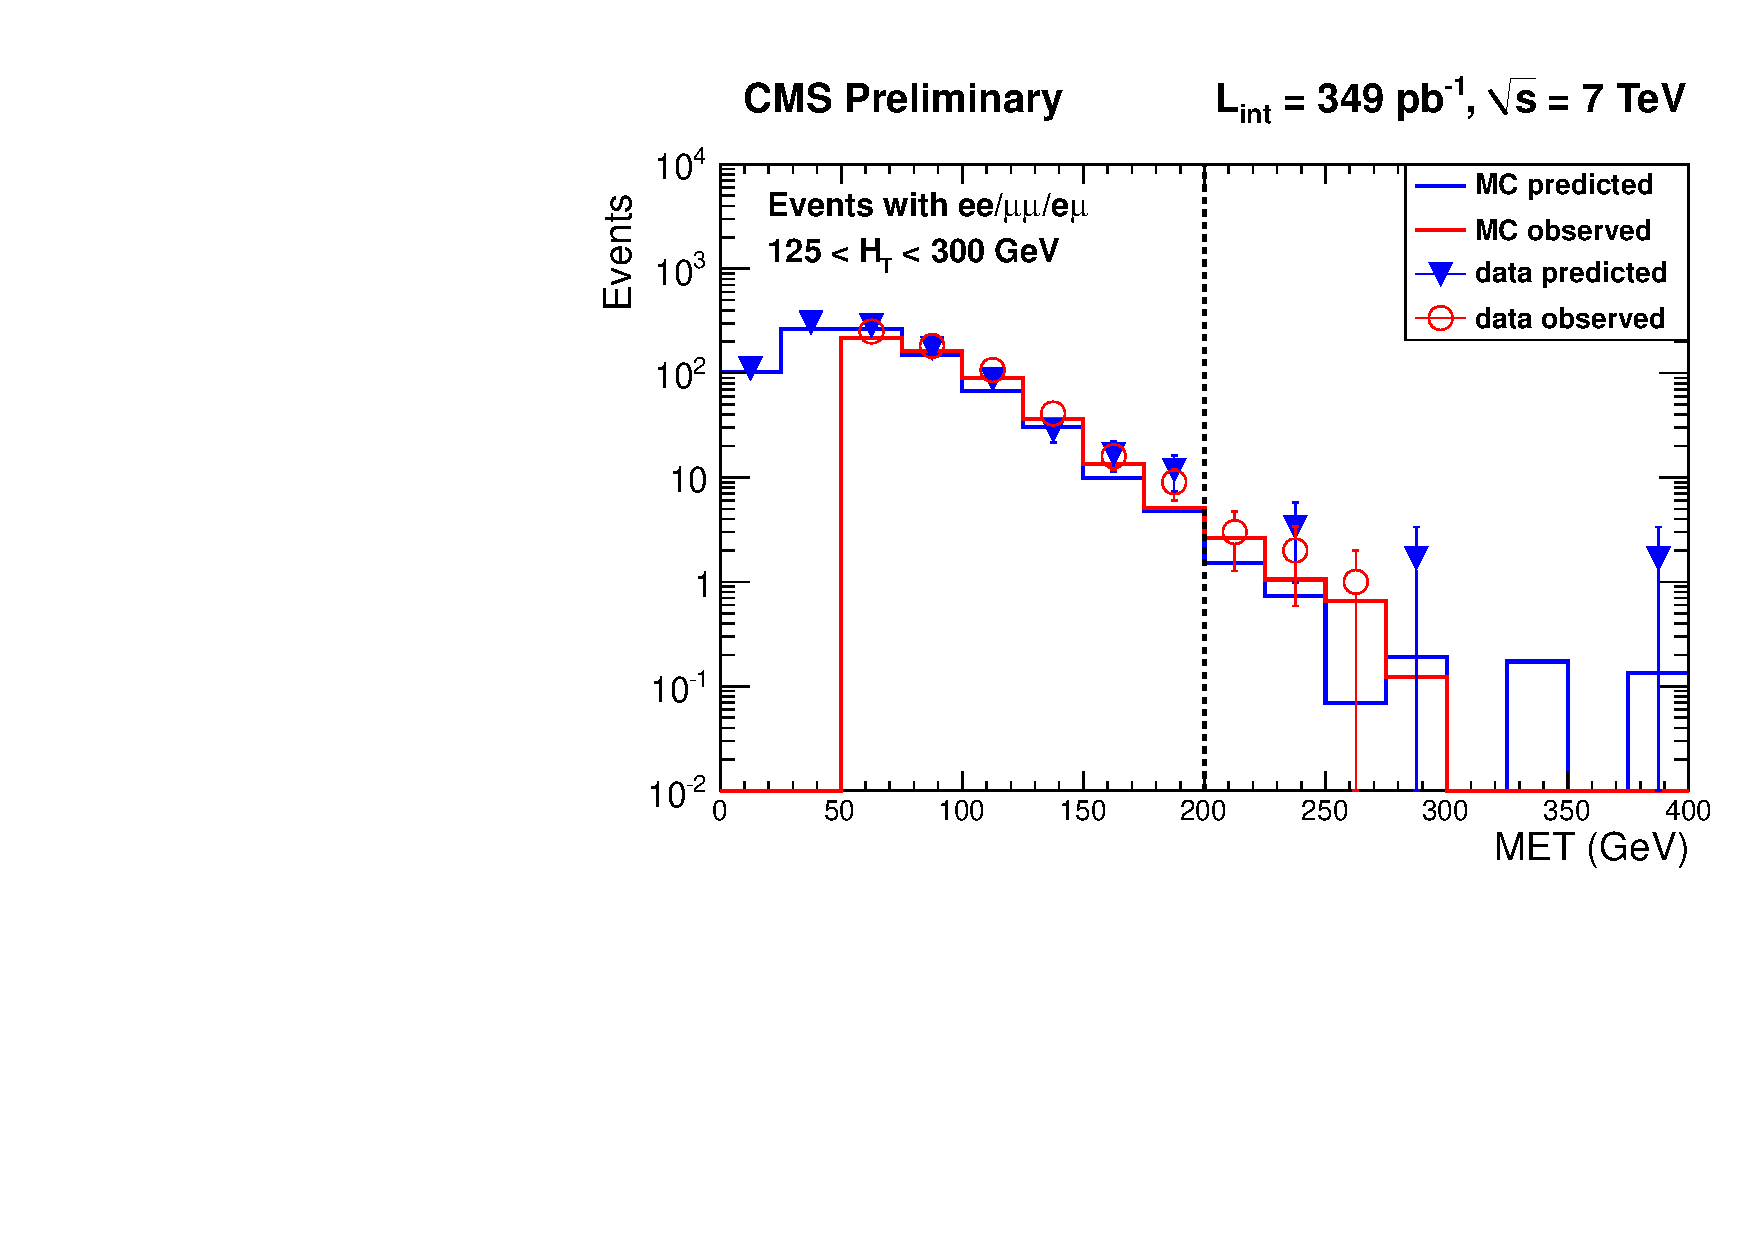
\includegraphics[width=0.48\linewidth]{plots/victory_met200_control_349pb.pdf}
\caption{\label{fig:victorycontrol}\protect 
Results of the \ptll\ method in the \Ht\ sideband region 125-300 GeV.
Left:  distributions of $\ptll/\sqrt{H_T}$ (predicted) and $y$ (observed) for 
SM MC and data. The vertical dashed lines indicate the requirement $y > 8.5$~GeV$^{1/2}$),
corresponding to the 2010 signal region.
Right: distributions of \ptll\ (predicted) and \met\ (observed) for 
SM MC and data. The vertical dashed lines indicate the requirement \met\ $>$ 200 GeV,
corresponding to the high \Ht\ signal region.
}
\end{center}
\end{figure}


\begin{figure}[tbh]
\begin{center}
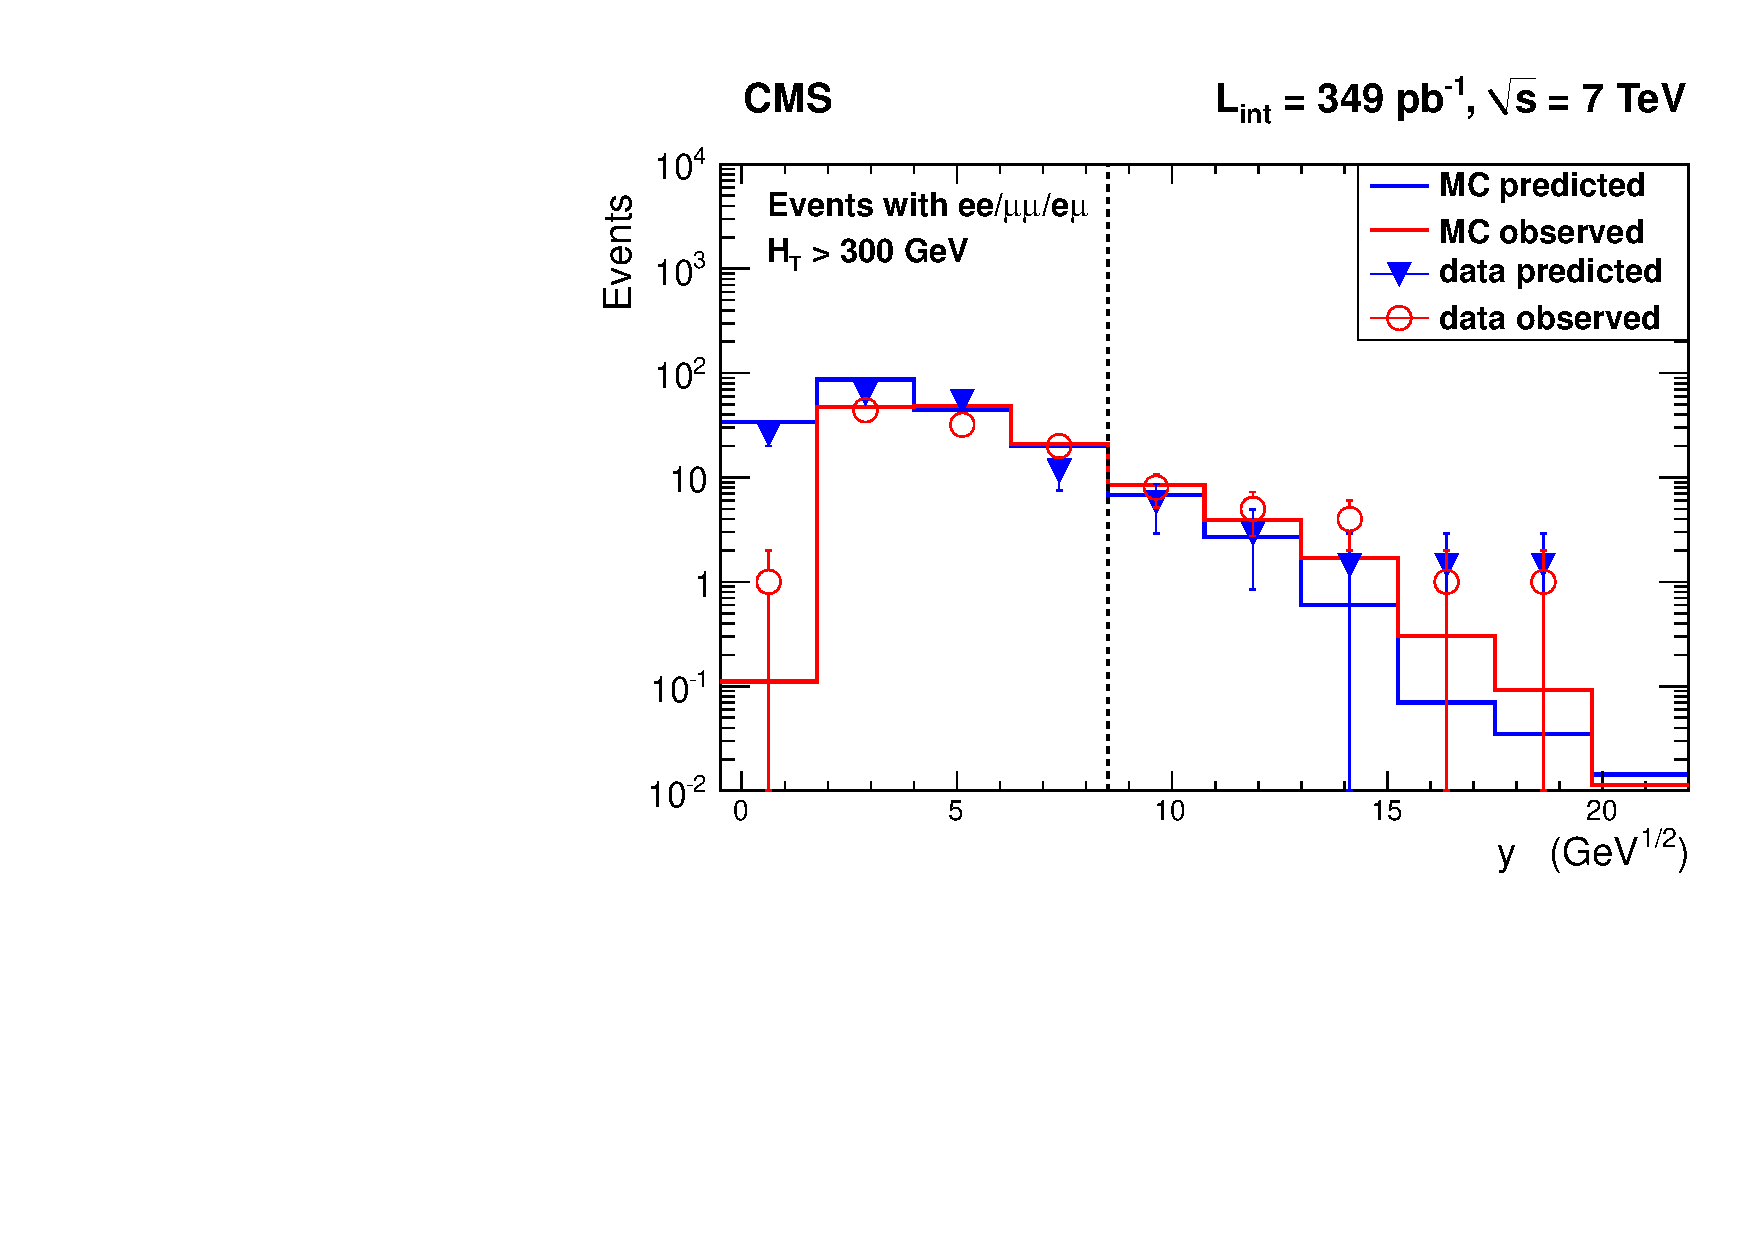
\includegraphics[width=0.6\linewidth]{plots/victory_y_ht300_349pb.pdf}
\caption{\label{fig:vic1}\protect 
Distributions of $\ptll/\sqrt{H_T}$ (predicted) and $y$ (observed) for 
SM MC and data, for the \Ht $>$ 300 GeV. 
The vertical dashed lines indicate the requirement $y > 8.5$~GeV$^{1/2}$ corresponding to the 2010 signal region.
}
\end{center}
\end{figure}

\begin{figure}[tbh]
\begin{center}
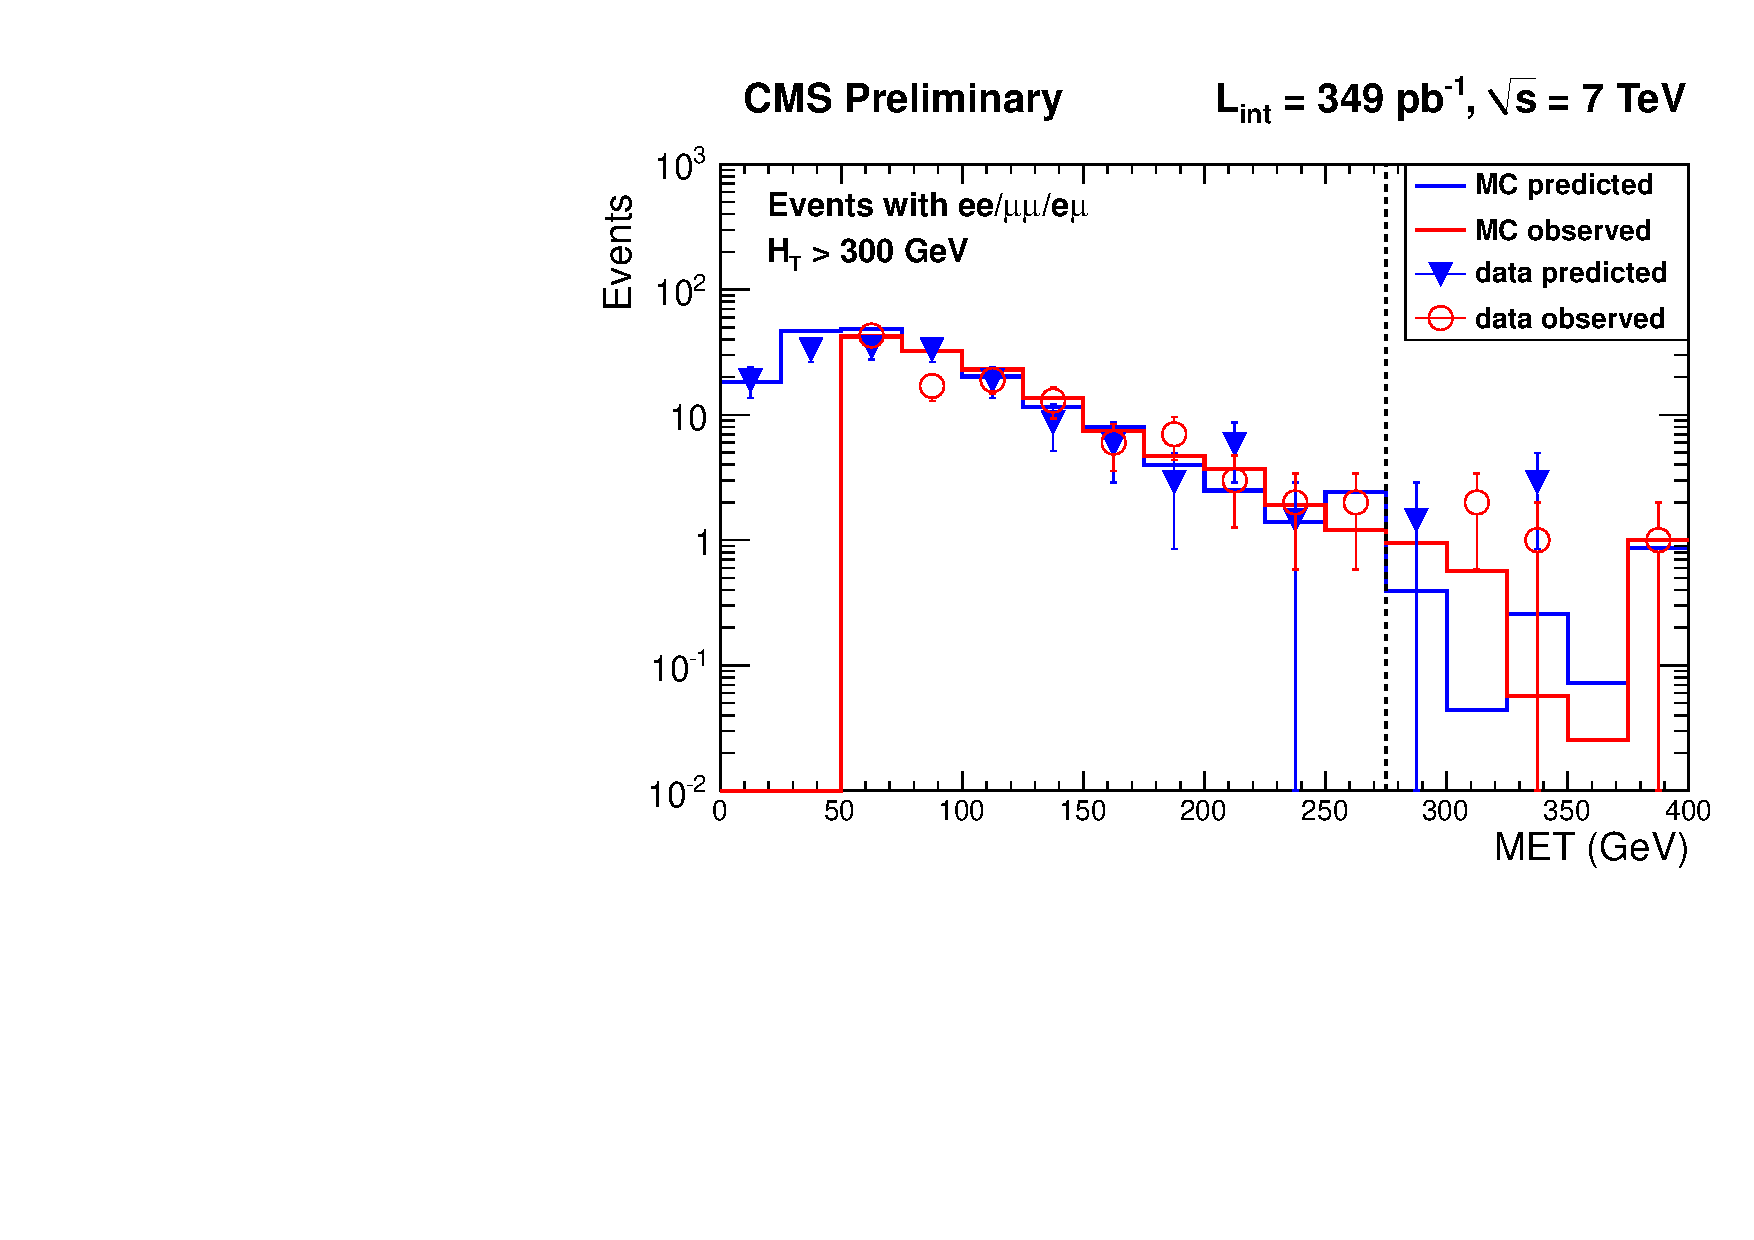
\includegraphics[width=0.6\linewidth]{plots/victory_met275_ht300_349pb.pdf}
\caption{\label{fig:v2}\protect 
Distributions of \ptll\ (predicted) and \met\ (observed) for 
SM MC and data, for the region \Ht $>$ 300 GeV. 
The vertical dashed lines indicate the requirement \met\ $>$ 275 GeV, corresponding to the high \met\ signal region.
}
\end{center}
\end{figure}

\begin{figure}[tbh]
\begin{center}
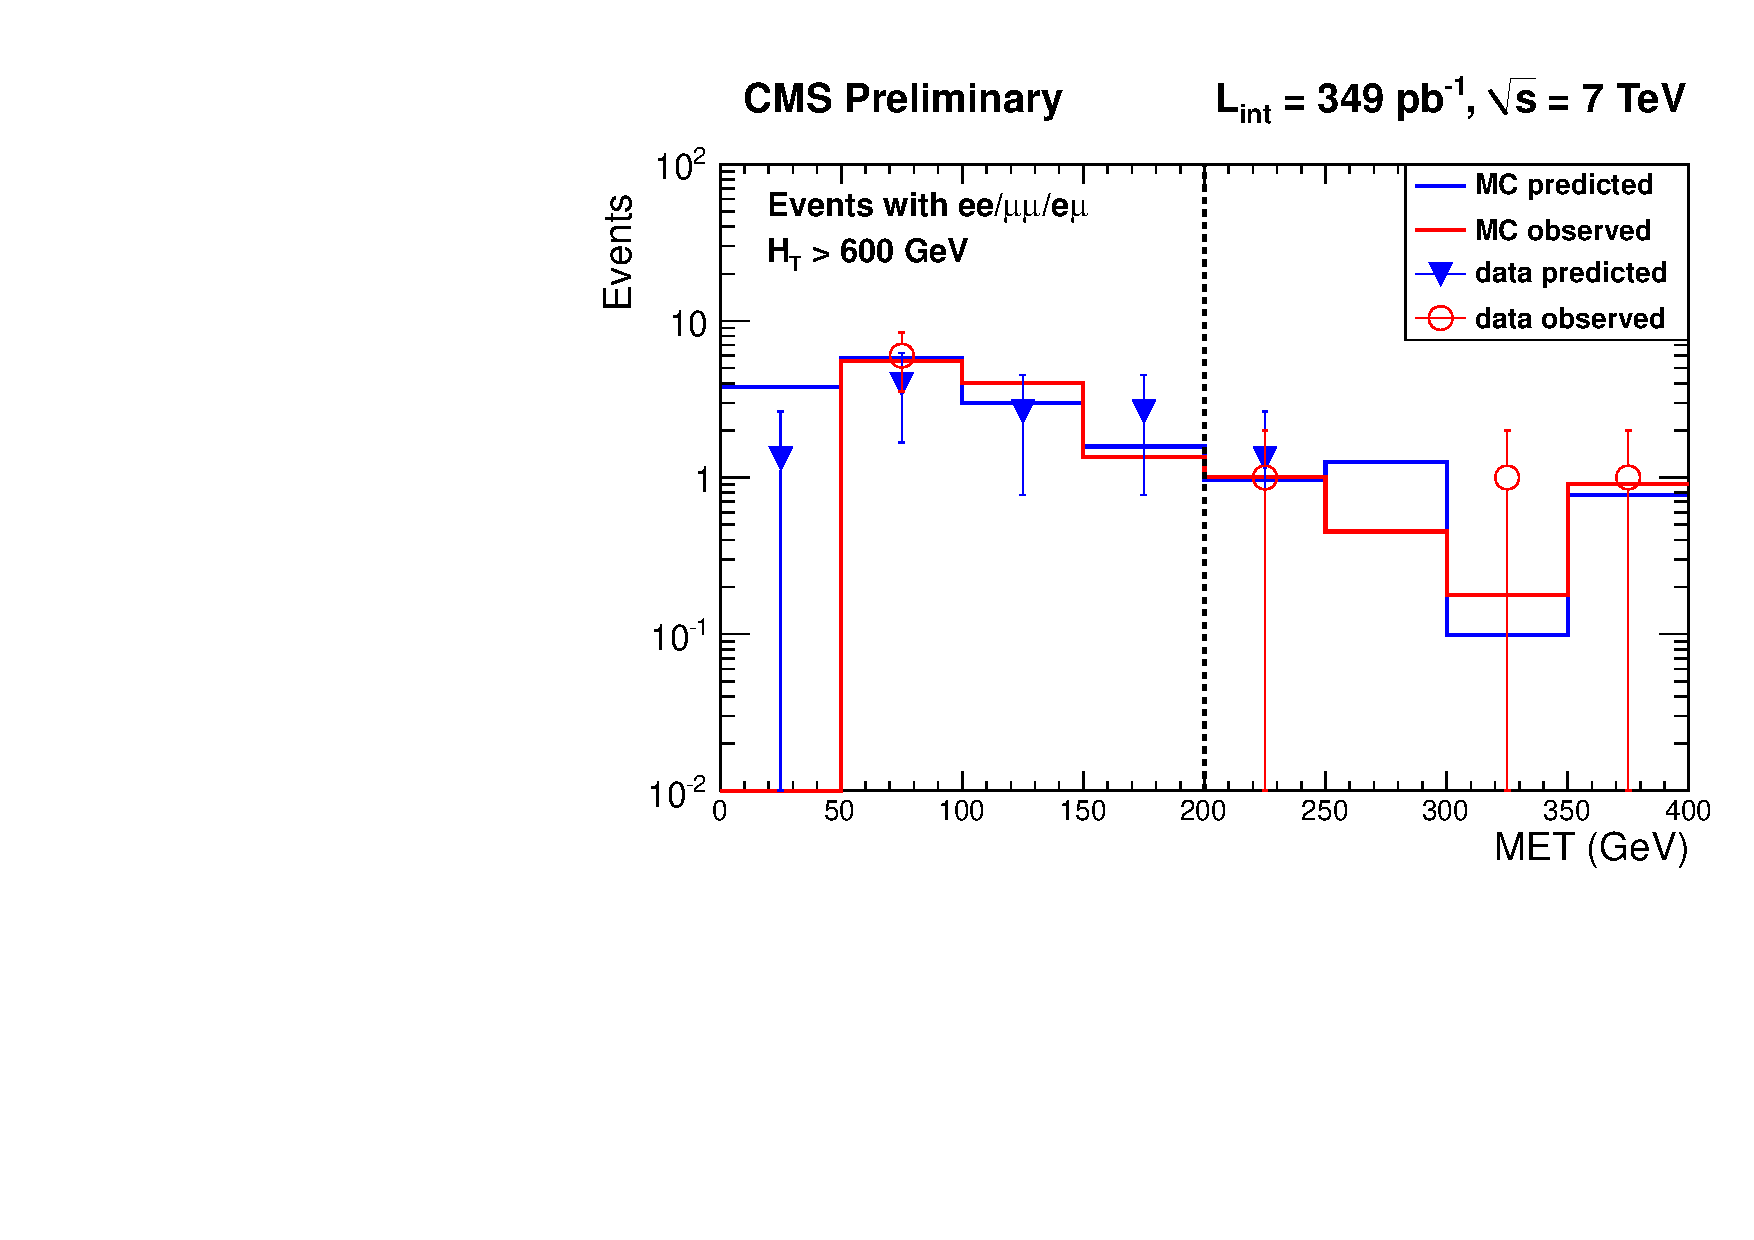
\includegraphics[width=0.6\linewidth]{plots/victory_met200_ht600_349pb.pdf}
\caption{\label{fig:vic3}\protect 
Distributions of \ptll\ (predicted) and \met\ (observed) for 
SM MC and data, for the region \Ht $>$ 600 GeV. 
The vertical dashed lines indicate the requirement \met\ $>$ 200 GeV, corresponding to the high \Ht\ signal region.
}
\end{center}
\end{figure}

\subsection{Background estimate from OF subtraction}
\label{sec:ofres}

The results of the OF subtraction technique applied to the high \pt\ dilepton trigger sample are summarized in Table~\ref{tab:ofres}. 
We evaluate the quantity $\Delta = R_{\mu e}N(ee) + \frac{1}{R_{\mu e}}N(\mu\mu) - N(e\mu)$ with $R_{\mu e} = 1.12 \pm 0.05$
extracted from the ratio of $Z \to \mu^+\mu^-$ vs. $Z \to e^+e^-$ events in data.
We perform the OF subtraction first in the preselection region, and find $\Delta$ consistent with 0, as expected.
We then perform the OF subtraction in all 3 signal regions, and do not observe any excess of same-flavor vs. opposite-flavor events.

\begin{table}[hbt]
\begin{center}
\caption{\label{tab:ofres} Summary of results for the OF subtraction technique. 
The quantity $\Delta = R_{\mu e}N(ee) + \frac{1}{R_{\mu e}}N(\mu\mu) - N(e\mu)$ is quoted with $R_{\mu e} = 1.12 \pm 0.05$.
The quoted systematic uncertainty corresponds to that of $R_{\mu e}$. The $e\mu$ yields differ from those previously
quoted because the $Z$ mass veto is included here.
}
\begin{tabular}{l|ccc|c}
\hline
region                   &  $N(ee)$ & $N(\mu\mu)$ & $N(e\mu)$  &  $\Delta$   \\ 
\hline
preselection region      &      193 &         201 &      394   &    2.0 $\pm$ 28 (stat) $\pm$ 1.8 (syst) \\    
2010 signal region       &        4 &           4 &        9   &   -0.9 $\pm$ 4.2 (stat) $\pm$ 0.1 (syst)  \\
high \met\ signal region &        2 &           0 &        1   &    1.3 $\pm$ 1.9 (stat) $\pm$ 0.1 (syst)  \\
high \Ht\ signal region  &        1 &           0 &        1   &    0.1 $\pm$ 1.5 (stat) $\pm$ 0.0 (syst)  \\
\hline
\end{tabular}
\end{center}
\end{table}

For the dilepton-\Ht\ trigger sample, we observe only 1 event in the 2010 signal region, consistent with MC expectations,
and no events in either the high $y$ or high \Ht\ signal regions. In the case of an excess of events at low lepton \pt,
we will perform the OF subtraction technique of Sec.~\ref{sec:oflowpt}.

% \clearpage
\subsection{Summary of results}

\begin{table}[hbt]
\begin{center}
\caption{\label{tab:results} 
Summary of the observed and predicted yields in the 3 signal regions. MC errors are statistical only. The systematic uncertainty on the ABCD
and \ptll\ method is from the scaling factors from MC closure only. 
%{\bf need to put additional uncertainties, for example jet/met scale.}
For the OF subtraction, the quantity $\Delta = R_{\mu e}N(ee) + \frac{1}{R_{\mu e}}N(\mu\mu) - N(e\mu)$ is quoted; the systematic uncertainty
here is from the ratio of muon to electron selection efficiencies.
}
\begin{tabular}{l|c|c|c}
\hline
                                       &  2010 signal region                       &   high \met\ signal region             &  high \Ht\ signal region              \\ 
\hline
Observed yield                         &         19                                &                        4               &                        3              \\
\hline
MC prediction                          &    14.5 $\pm$ 1.4                         &            2.6 $\pm$ 0.8               &            2.5 $\pm$ 0.8              \\
ABCD prediction                        &    12.7 $\pm$ 2.4 (stat) $\pm$ 2.5 (syst) &                                        &                                       \\
ABCD' prediction                       &    12.8 $\pm$ 2.9 (stat) $\pm$ 2.6 (syst) & 1.2 $\pm$ 0.4 (stat) $\pm$ 0.5 (syst)  & 0.0 $\pm$ 0.6 (stat) $\pm$ 0.3 (syst) \\
\ptll\ prediction                      &    16.7 $\pm$ 6.1 (stat) $\pm$ 5.9 (syst) & 5.4 $\pm$ 3.8 (stat) $\pm$ 2.2 (syst)  & 1.7 $\pm$ 1.7 (stat) $\pm$ 0.6 (syst) \\
\hline
OF subtraction ($\Delta$)              &    -0.9 $\pm$ 4.2 (stat) $\pm$ 0.1 (syst) & 1.3 $\pm$ 1.9 (stat) $\pm$ 0.1 (syst)  & 0.1 $\pm$ 1.5 (stat) $\pm$ 0.0 (syst) \\
\hline
\end{tabular}
\end{center}
\end{table}

A summary of our results is presented in Table~\ref{tab:results}. In all 3 signal regions, we observe reasonable agreement
between the observed yields and the predictions from MC and data-driven background estimates. We therefore do not observe
evidence for an excess of events above SM expectations. After assessing systematic uncertainties in Sec.~\ref{sec:systematics},
we proceed to set upper limits on the non-SM contributions to the signal regions in Sec.~\ref{sec:limits}.
 
%\section{Interpretation}
\label{sec:interpretation}

In this section, we interpret the results of the targeted search in the context of the \wzmet\ model depicted in Fig.~\ref{fig:diagrams} (right)
and a gauge-mediated SUSY breaking (GMSB) model that produces a signature of \zzmet\ will be added. The results of the targeted search presented here
will be combined with those of the trilepton ewkino search for the final \wzmet\ interpretation, and with the quadlepton ewkino search
for the final GMSB \zzmet\ interpretation.

The exclusion is performed using the results of simultaneous counting experiments in the five exclusive \MET\ signal regions defined by \MET\ $>$ 80 GeV,
as summarized in Table~\ref{tab:results_targ} (commonly referred to as a ``shape analysis''). 
The upper limit calculation is performed with the LandS software using the LHC-type CLs criterion.
The signal efficiency uncertainties include the luminosity (4.4\%), acceptance for the b-jet veto (4\%), lepton ID and isolation efficiency (2\% per lepton),
and trigger efficiency (3\%). The uncertainty from JES is determined following the POG-recommended procedure, by varying the jet energies by the 
\pt- and $\eta$-dependent uncertainties and propagating this to the jet multiplicity, dijet mass, and \MET.
The background uncertainties are quoted in Table~\ref{tab:results_targ}. For each background contribution, the uncertainty is assumed to be 100\% 
correlated across all signal regions.

For the \wzmet\ model, the signal efficiency times acceptance and cross section upper limits are displayed in Fig.~\ref{fig:results_wzmet},
along with the observed and expected exclusion contours, which are compared to the 2011 observed exclusion contour.
Figure~\ref{fig:results_wzmetpoints} shows the excluded points used to derive the exclusion contours. We note that the map of exclusion
contours appears quite ragged since for many of the points the cross section upper limit is very close to the theory cross section.
Therefore we do not expect the ragged exclusion region to be an issue for the final results since
we currently have 9.2 fb$^{-1}$ and expect the luminosity to increase significantly. A {\bf VERY APPROXIMATE} projection of the expected excluded region
for an integrated luminosity of 15 fb$^{-1}$ (a rough guess at the final HCP data sample) is obtained by scaling the expected cross section limits by 
$\sqrt{(9.2 \rm{fb}^{-1})/(15 \rm{fb}^{-1})}$, as displayed in Fig.~\ref{fig:results_15fb}.

\begin{figure}[!ht]
\begin{center}
\begin{tabular}{cc}
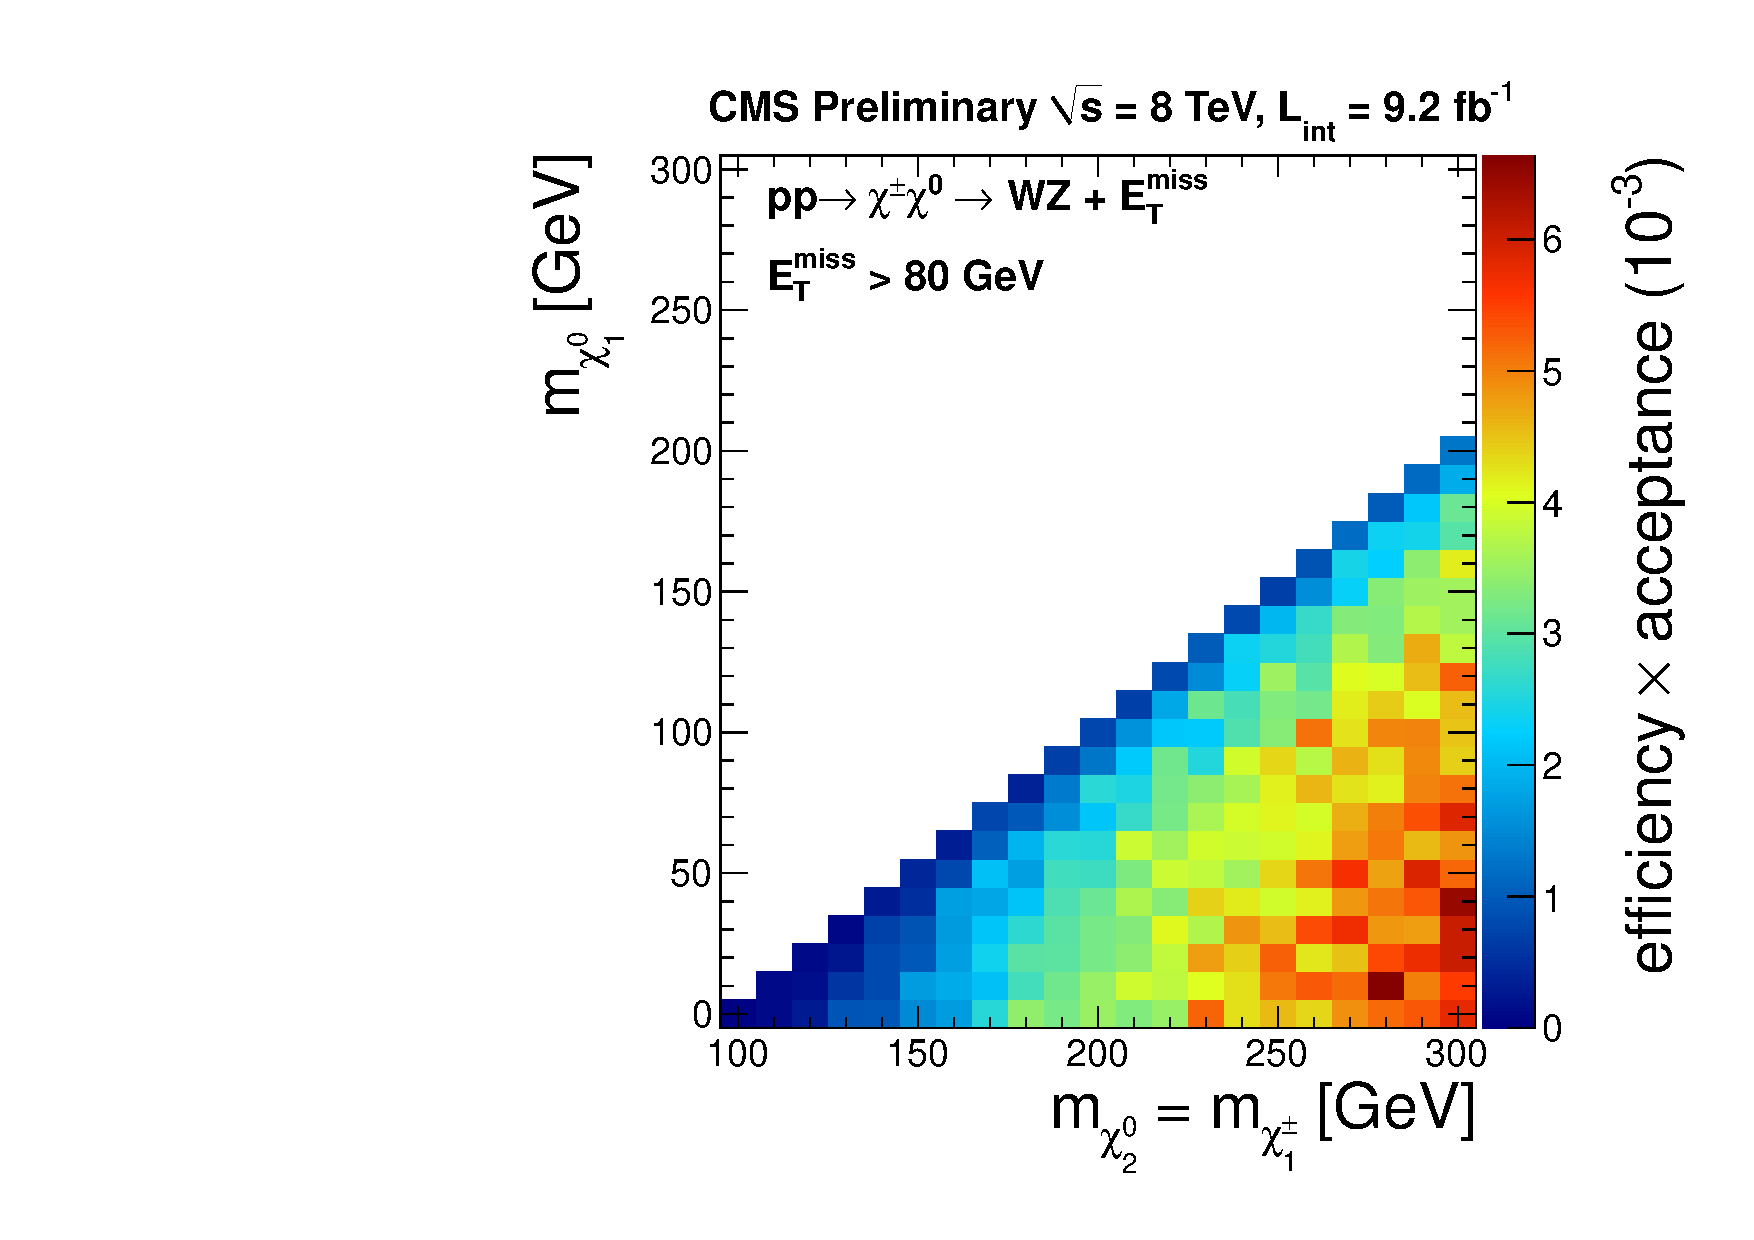
\includegraphics[width=0.45\textwidth]{plots/wzsms_eff.pdf}
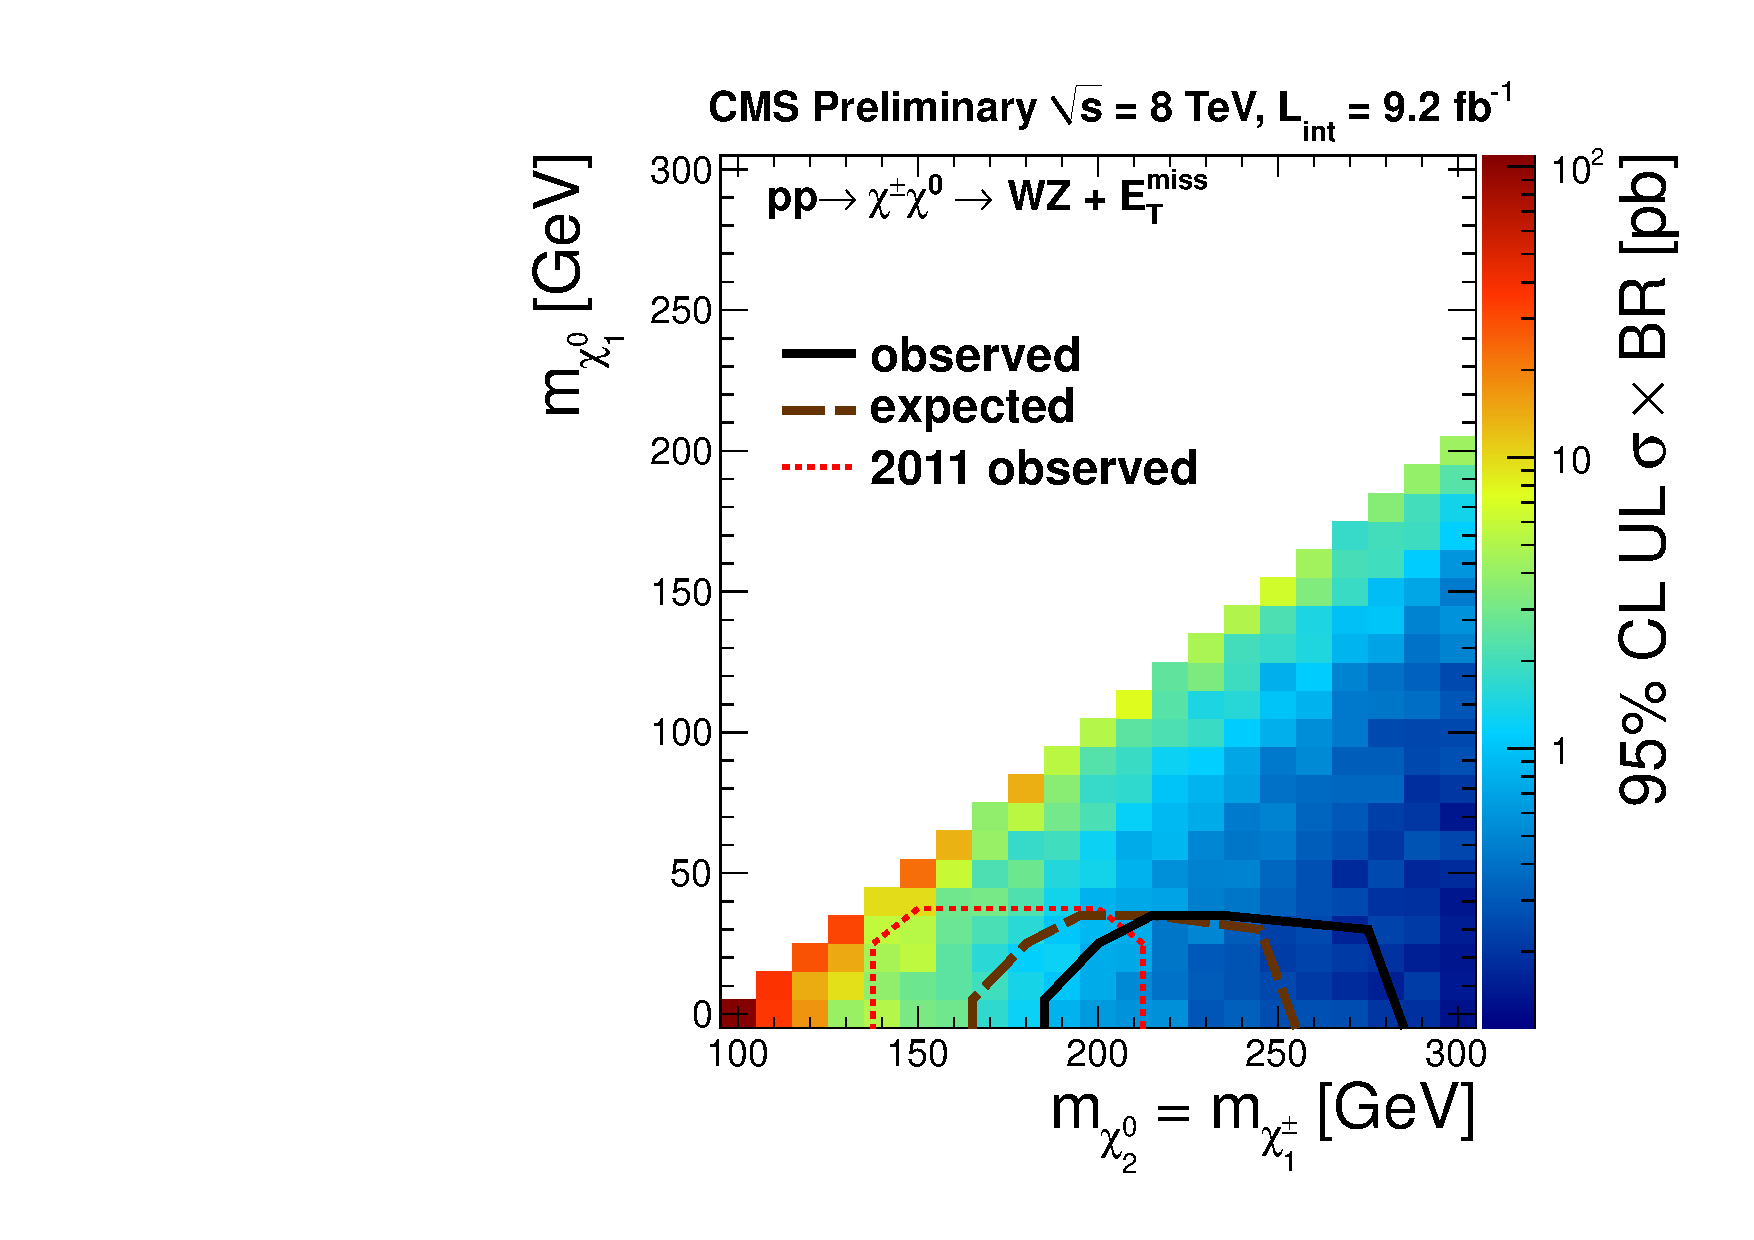
\includegraphics[width=0.45\textwidth]{plots/wzsms_xsec.pdf}
\end{tabular}
\caption{ Interpretation of the targeted analysis in the \wzmet\ model. The acceptance times efficiency (left) and cross section
upper limit (right) and displayed. The observed and expected exclusion contours are indicated and compared to the observed
exclusion from the 2011 analysis.
\label{fig:results_wzmet}}
\end{center}
\end{figure}

\begin{figure}[!hb]
\begin{center}
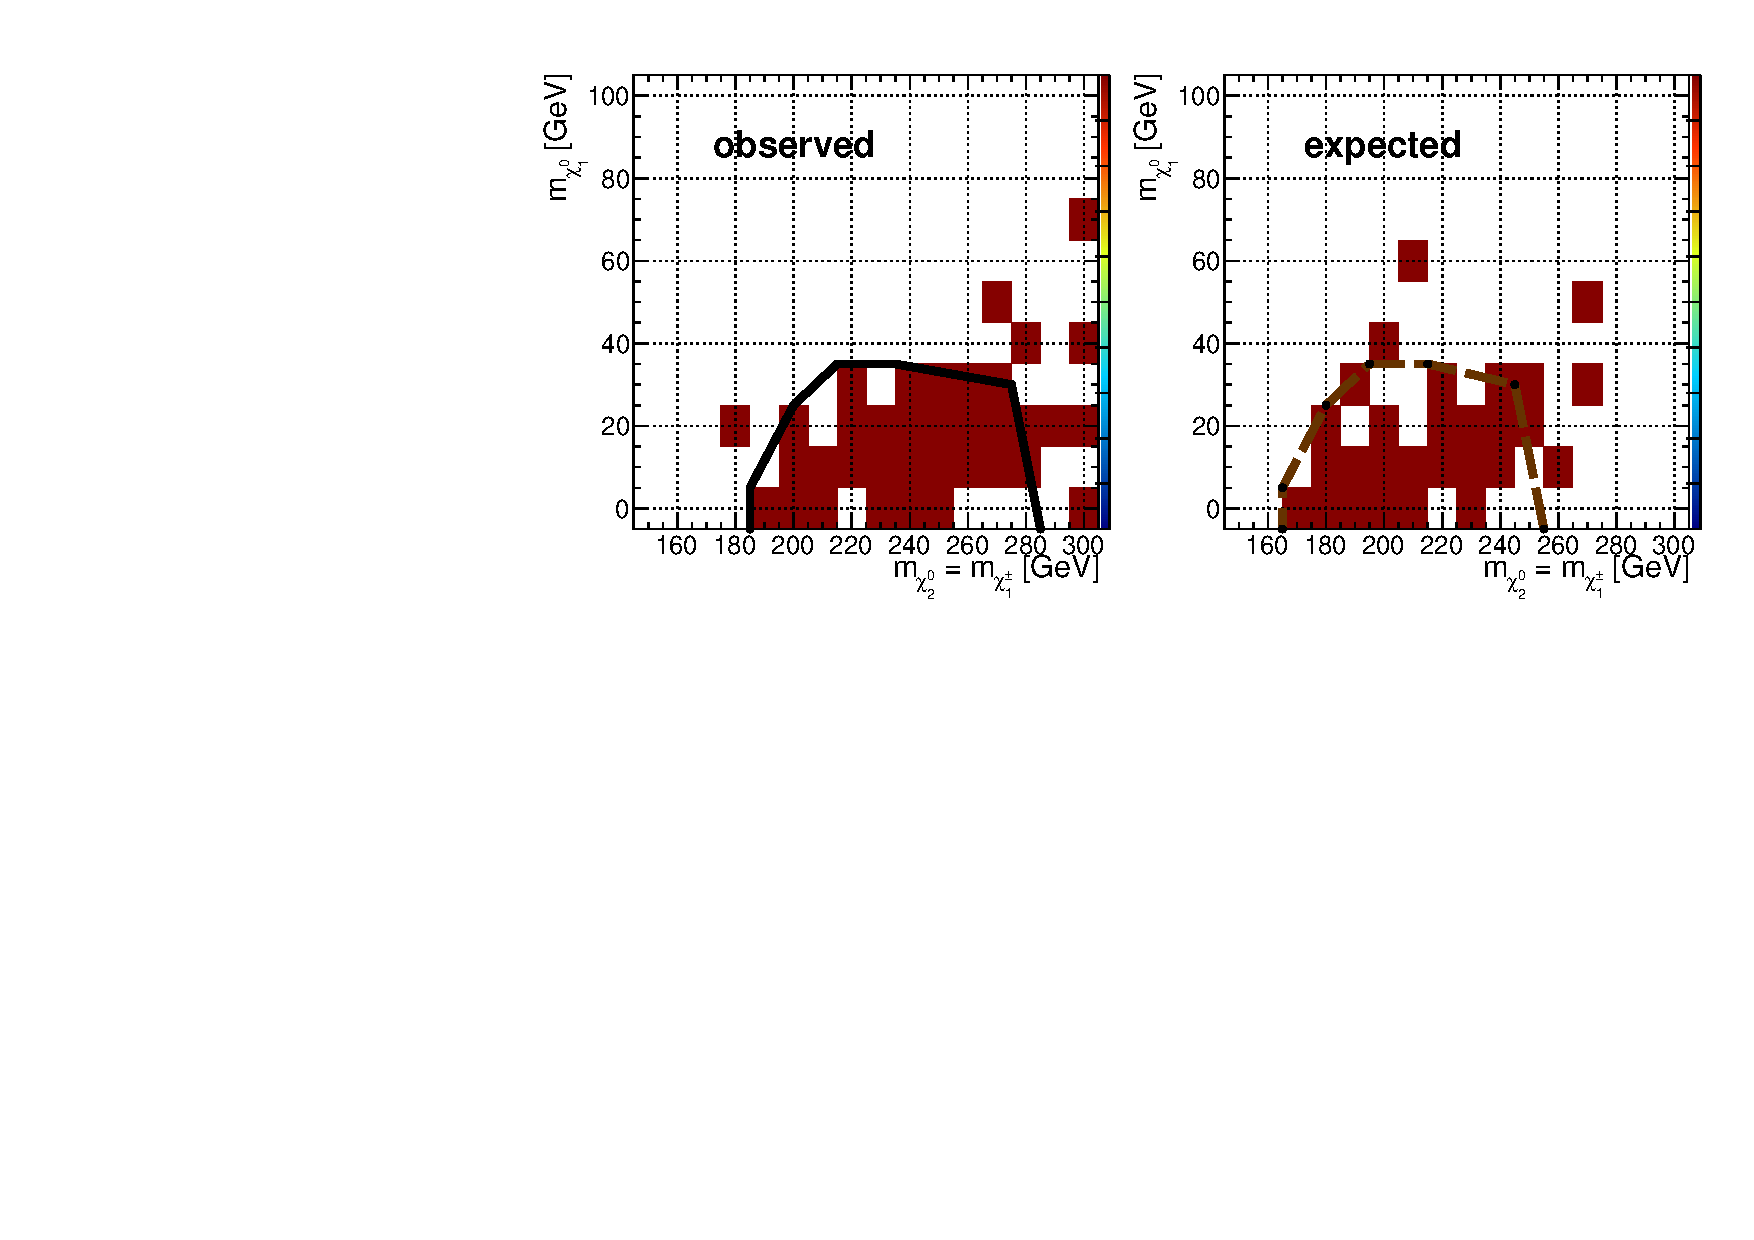
\includegraphics[width=0.75\textwidth]{plots/wzsms_points.pdf}
\caption{ Observed (left) and expected (right) excluded points for the \wzmet\ interpretation, with the corresponding exclusion contours overlaid.
\label{fig:results_wzmetpoints}}
\end{center}
\end{figure}

\clearpage

\begin{figure}[!ht]
\begin{center}
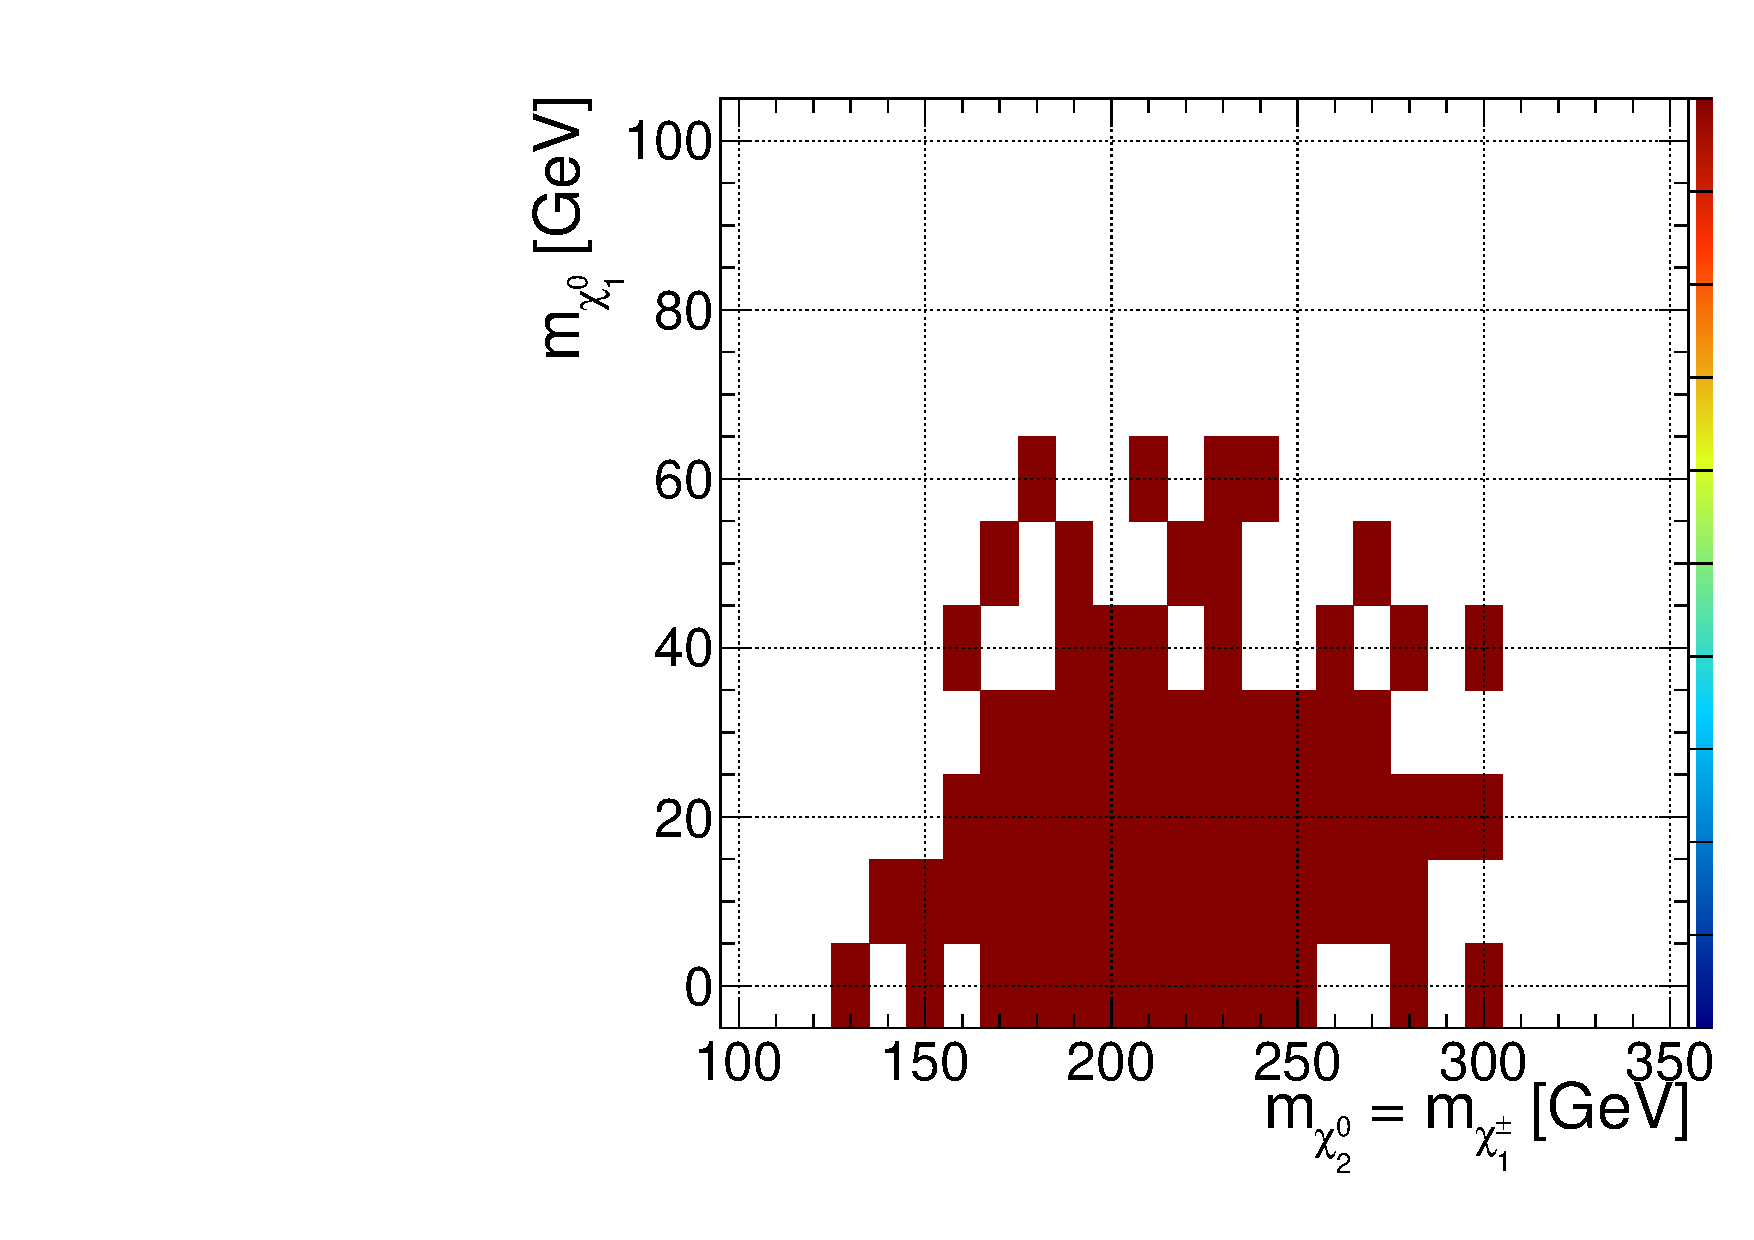
\includegraphics[width=0.5\textwidth]{plots/wzsms_expected_15fb.pdf}
\caption{ A {\bf VERY APPROXIMATE} projection of the expected excluded points for an integrated luminosity of 15$^{-1}$. 
\label{fig:results_15fb}}
\end{center}
\end{figure}

The results of the interpretation in the GMSB \zzmet\ model are displayed in Fig.~\ref{fig:results_gmsb},
as a function of the chargino and neutralino mass parameter $\mu$. These results exclude the range $196 < \mu < 316$~GeV.

\begin{figure}[!hb]
\begin{center}
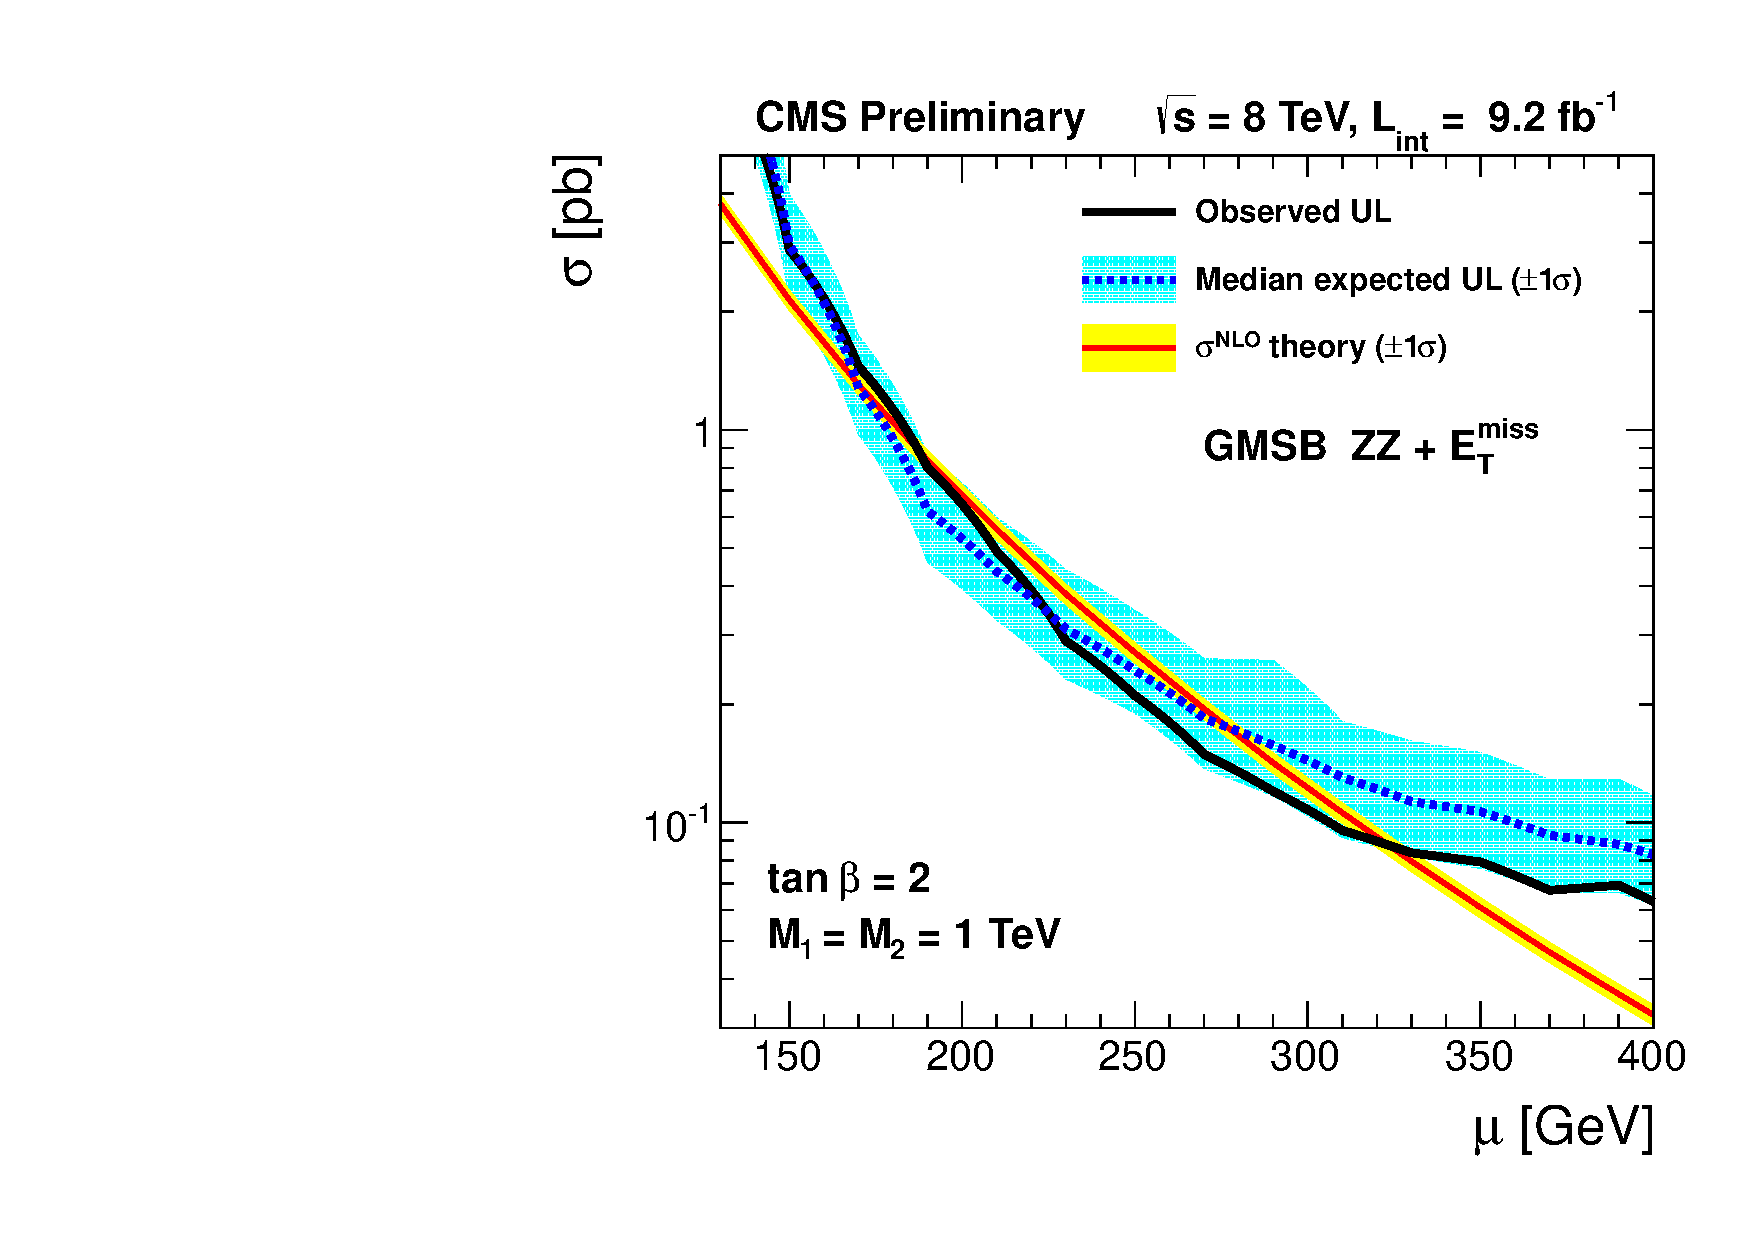
\includegraphics[width=0.5\textwidth]{plots/ZDIJET_GMSB.pdf}
\caption{ Interpretation of the targeted analysis in the GMSB \zzmet\ model.
\label{fig:results_gmsb}}
\end{center}
\end{figure}
 
\section{Summary}

This note presents a search for BSM physics in final states with leptonically-decaying Z bosons, jets, and \MET. 
Two strategies were pursued. The first is an inclusive approach which targets BSM scenarios with Z bosons produced
in the decays of strongly-interacting particles. The second is a targeted approach which focuses on BSM scenarios
where the Z bosons are produced in the decays of weakly-interacting particles. The main backgrounds are
estimated with data-driven techniques. Good agreement is observed between the data and the predicted backgrounds
over the full \MET\ range, for both searches. The results are interpreted in the context of a simplified SUSY
model where chargino-neutralino pairs decay to the \wzmet\ final state, and used to place constraints on the
masses of these particles.


\clearpage
\begin{thebibliography}{10}
%  \bibitem {NOTE000} {\bf CMS Note 2005/000},
%    X.Somebody et al.,
%    {\em "CMS Note Template"}.

\bibitem{ref:Ztemplates} ADD REF TO MET TEMPLATES NOTE, WHEN AVAILABLE

\bibitem{ref:osnote} CMS AN-2010/370

\bibitem{ref:ospaper} arXiv:1103.1348v1 [hep-ex], ``Search for Physics Beyond the Standard Model in Opposite-Sign Dilepton Events at $\sqrt{s} = 7$~TeV.''

\bibitem{ref:top} Phys.Lett.B695:424-443,2011 

\bibitem{ref:vbtf} https://twiki.cern.ch/twiki/bin/viewauth/CMS/SimpleCutBasedEleID

\bibitem{ref:conv} D.~Barge {\em at al.}, AN-CMS2009/159.

\bibitem{ref:xsec} https://twiki.cern.ch/twiki/bin/view/CMS/ProductionReProcessingSpring10 
% {\color{red} Is this the right reference?}


\bibitem{ref:victory}V.~Pavlunin, Phys. Rev. {\bf D81}, 035005 (2010).

\bibitem{ref:ourvictory}  D.~Barge {\em at al.}, AN-CMS2009/130.

\bibitem{ref:dy} W.~Andrews {\em et al.}, AN-CMS2009/023.

\bibitem{ref:FR} D.~Barge {\em at al.}, AN-CMS2010/257.

\bibitem{ref:evans}W.~Andrews {\em et al.}, AN-CMS2010/274.

\bibitem{ref:bayes.f} J.~Conway, {\tt http://www-cdf.fnal.gov/physics/statistics/code/bayes.f}.

\bibitem{ref:cl95cms} G.~Landsberg, {\tt https://twiki.cern.ch/twiki/pub/CMS/EXOTICA/cl95cms.c}

\bibitem{ref:scan} {\tt https://hypernews.cern.ch/HyperNews/CMS/get/susy/617/2/1.html}

\bibitem{ref:sanjay} {\tt https://twiki.cern.ch/twiki/bin/view/CMS/SUSY38XSUSYScan}

\bibitem{ref:pdf} arXiv:hep-ph/0605240v2

\bibitem{ref:smooth} {\tt CleanExclusion.cc} available at
{\tt https://twiki.cern.ch/twiki/bin/viewauth/CMS/SUSYLimitTools}

\bibitem{ref:cousins} R.~Cousins, {\tt http://www.physics.ucla.edu/\~cousins/stats/cousins\_lognormal\_prior.pdf}

\bibitem{ref:harper} S.~Harper, private communication (relayed to us by M.~Chiorboli.).

\bibitem{ref:MT2} A. Barr {\em at al.}, J.Phys.G29:2343-2363,2003;
Cheng, H.C., Han, arXiv:hep-ph/0810.5178v2.\\
{\tt http://indico.cern.ch/contributionDisplay.py?contribId=3\&confId=66410}

\bibitem{ref:MT2J} {\tt http://indico.cern.ch/contributionDisplay.py?contribId=5\&confId=93837}

\bibitem{ref:brown} M.~Narain {\em et al.}, CMS AN-2010/259; we thank the 
Brown group for providing their code to us.


    
\end{thebibliography}


\appendix
\clearpage

\section{Results in the ee and $\mu\mu$ Channels}
\label{app:results}

In this section we provide the results of the inclusive and targeted searches, separately in the ee and $\mu\mu$ channels.
The \MET\ distributions in the inclusive analysis for the ee channel are displayed in Fig.~\ref{fig:results_incl_ee} and 
the signal region yields are presented in Table~\ref{tab:results_incl_ee}.
The \MET\ distributions in the inclusive analysis for the $\mu\mu$ channel are displayed in Fig.~\ref{fig:results_incl_mm} and 
the signal region yields are presented in Table~\ref{tab:results_incl_mm}.

\begin{figure}[!h]
\begin{center}
\begin{tabular}{cc}
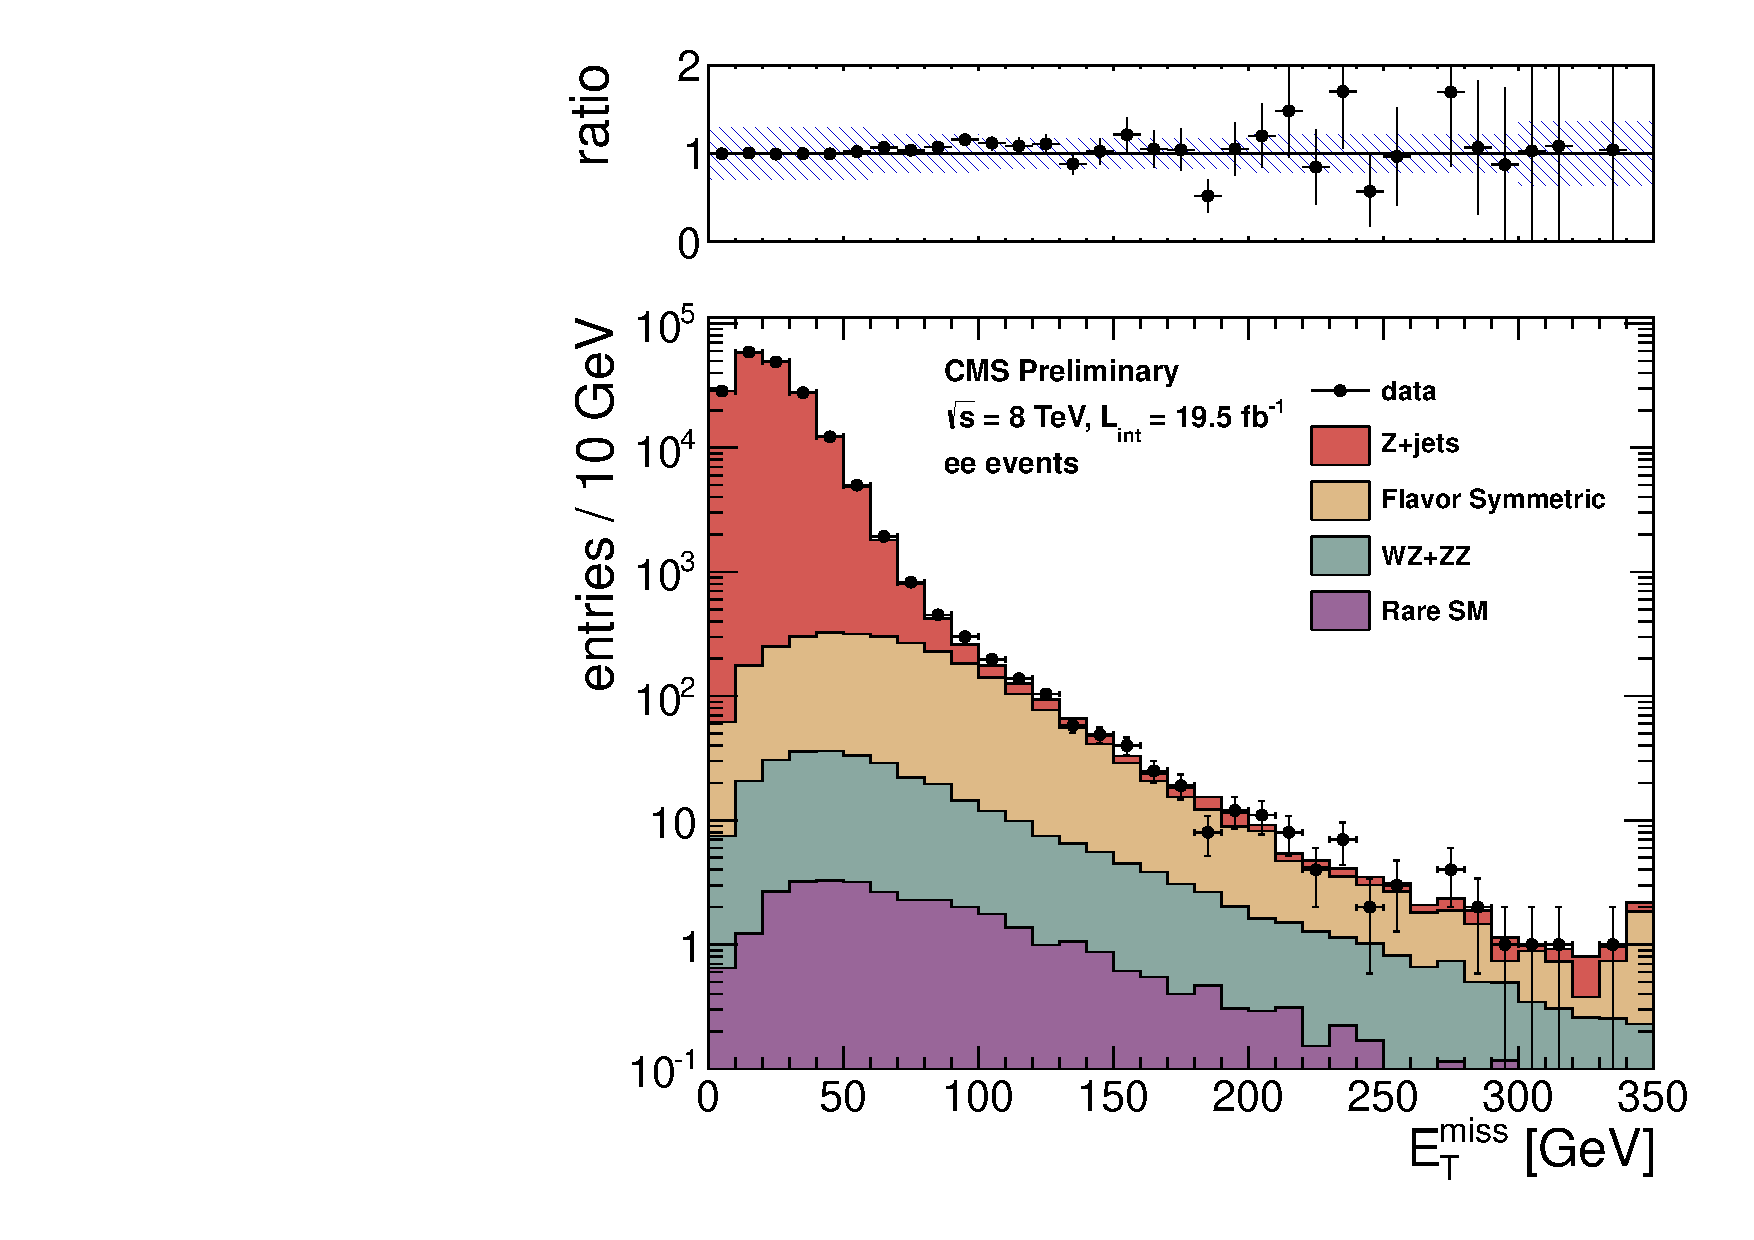
\includegraphics[width=0.6\textwidth]{plots/pfmet_ee_19p5fb.pdf}
\end{tabular}
\caption{Results of the inclusive analysis in the ee channel. The observed \MET\ distribution (black points) is compared with the sum of the predicted \MET\
distributions from \zjets, flavor-symmetric backgrounds, and WZ+ZZ backgrounds. The ratio of observed to predicted yields in each bin is
indicated. The error bars indicate the statistical uncertainty in the data and the shaded band indicates the total background uncertainty.
\label{fig:results_incl_ee}
}
\end{center}
\end{figure}

\begin{table}[htb]
\begin{center}
\footnotesize
\caption{\label{tab:results_incl_ee} Summary of results in the inclusive analysis in the ee channel. The total background is the sum of the \zjets\ background predicted from
the \MET\ templates method (\zjets\ bkg), the flavor-symmetric background predicted from e$\mu$ events (FS bkg), and the WZ and ZZ backgrounds predicted from MC
(WZ bkg and ZZ bkg). All uncertainties include both the statistical and systematic components. The Gaussian significance of the deviation between the data 
and total background is indicated for signal regions with at least 20 observed events. }
\begin{tabular}{l|c|c|c|c|c|c}

\hline
\hline

%ee channel: scale em yield by 0.43
%Yields in 0-60 GeV region
%data   : 181351
%gjets  : 183192
%OF     : 1268.53
%WZ     : 132.629
%ZZ     : 17.1901
%Rare   : 14.2168
%Scaling gjets by : 0.982131
%SF events 185555
%OF events 43832

%ee events

                      &   \MET\ 0--30 GeV   &  \MET\ 30--60 GeV   & \MET\ 60--100 GeV   &\MET\ 100--200 GeV   &\MET\ 200--300 GeV   & \MET\ $>$ 300 GeV  \\
\hline
        \zjets\ bkg   &136452 $\pm$ 40942   & 43466 $\pm$ 13049   &    2220 $\pm$ 675   &      100 $\pm$ 57   &     5.1 $\pm$ 1.6   &     1.2 $\pm$ 0.4  \\
             FS bkg   &      431 $\pm$ 81   &     838 $\pm$ 156   &     896 $\pm$ 167   &      448 $\pm$ 84   &    22.5 $\pm$ 7.1   &     3.2 $\pm$ 1.9  \\
             WZ bkg   &   49.0 $\pm$ 24.5   &   83.6 $\pm$ 41.8   &   62.6 $\pm$ 31.3   &   35.7 $\pm$ 17.9   &     5.2 $\pm$ 2.6   &     1.5 $\pm$ 1.5  \\
             ZZ bkg   &     5.3 $\pm$ 2.7   &    11.9 $\pm$ 6.0   &    13.2 $\pm$ 6.6   &    13.3 $\pm$ 6.7   &     3.0 $\pm$ 1.5   &     0.9 $\pm$ 0.9  \\
        rare SM bkg   &     4.5 $\pm$ 2.3   &     9.7 $\pm$ 4.9   &     9.2 $\pm$ 4.6   &     8.4 $\pm$ 4.2   &     1.7 $\pm$ 0.8   &     0.5 $\pm$ 0.5  \\
\hline
          total bkg   &136942 $\pm$ 40942   & 44409 $\pm$ 13050   &    3201 $\pm$ 696   &     606 $\pm$ 103   &    37.3 $\pm$ 7.9   &     7.3 $\pm$ 2.7  \\
               data   &            136404   &             44947   &              3508   &               651   &                42   &                 3  \\
%       significance   &      -0.0$\sigma$   &       0.0$\sigma$   &       0.4$\sigma$   &       0.4$\sigma$   &       0.5$\sigma$   &      -1.3$\sigma$  \\
\hline
\hline


%float Zbkg_yield[nbins]    = { 100.4 ,  5.1 ,     1.2  };
%float Zbkg_err[nbins]      = { 57.1 ,  1.6 ,     0.4  };
%float OFbkg_yield[nbins]   = { 448.4 , 22.5 ,     3.2  };
%float OFbkg_err[nbins]     = { 83.8 ,  7.1 ,     1.9  };
%float WZbkg_yield[nbins]   = { 35.7 ,  5.2 ,     1.5  };
%float WZbkg_err[nbins]     = { 17.9 ,  2.6 ,     1.5  };
%float ZZbkg_yield[nbins]   = { 13.3 ,  3.0 ,     0.9  };
%float ZZbkg_err[nbins]     = {  6.7 ,  1.5 ,     0.9  };
%float rarebkg_yield[nbins] = {  8.4 ,  1.7 ,     0.5  };
%float rarebkg_err[nbins]   = {  4.2 ,  0.8 ,     0.5  };
%int   data_yield[nbins]    = {  651 ,   42 ,       3  };


\end{tabular}
\end{center}
\end{table}

\clearpage

\begin{figure}[!h]
\begin{center}
\begin{tabular}{cc}
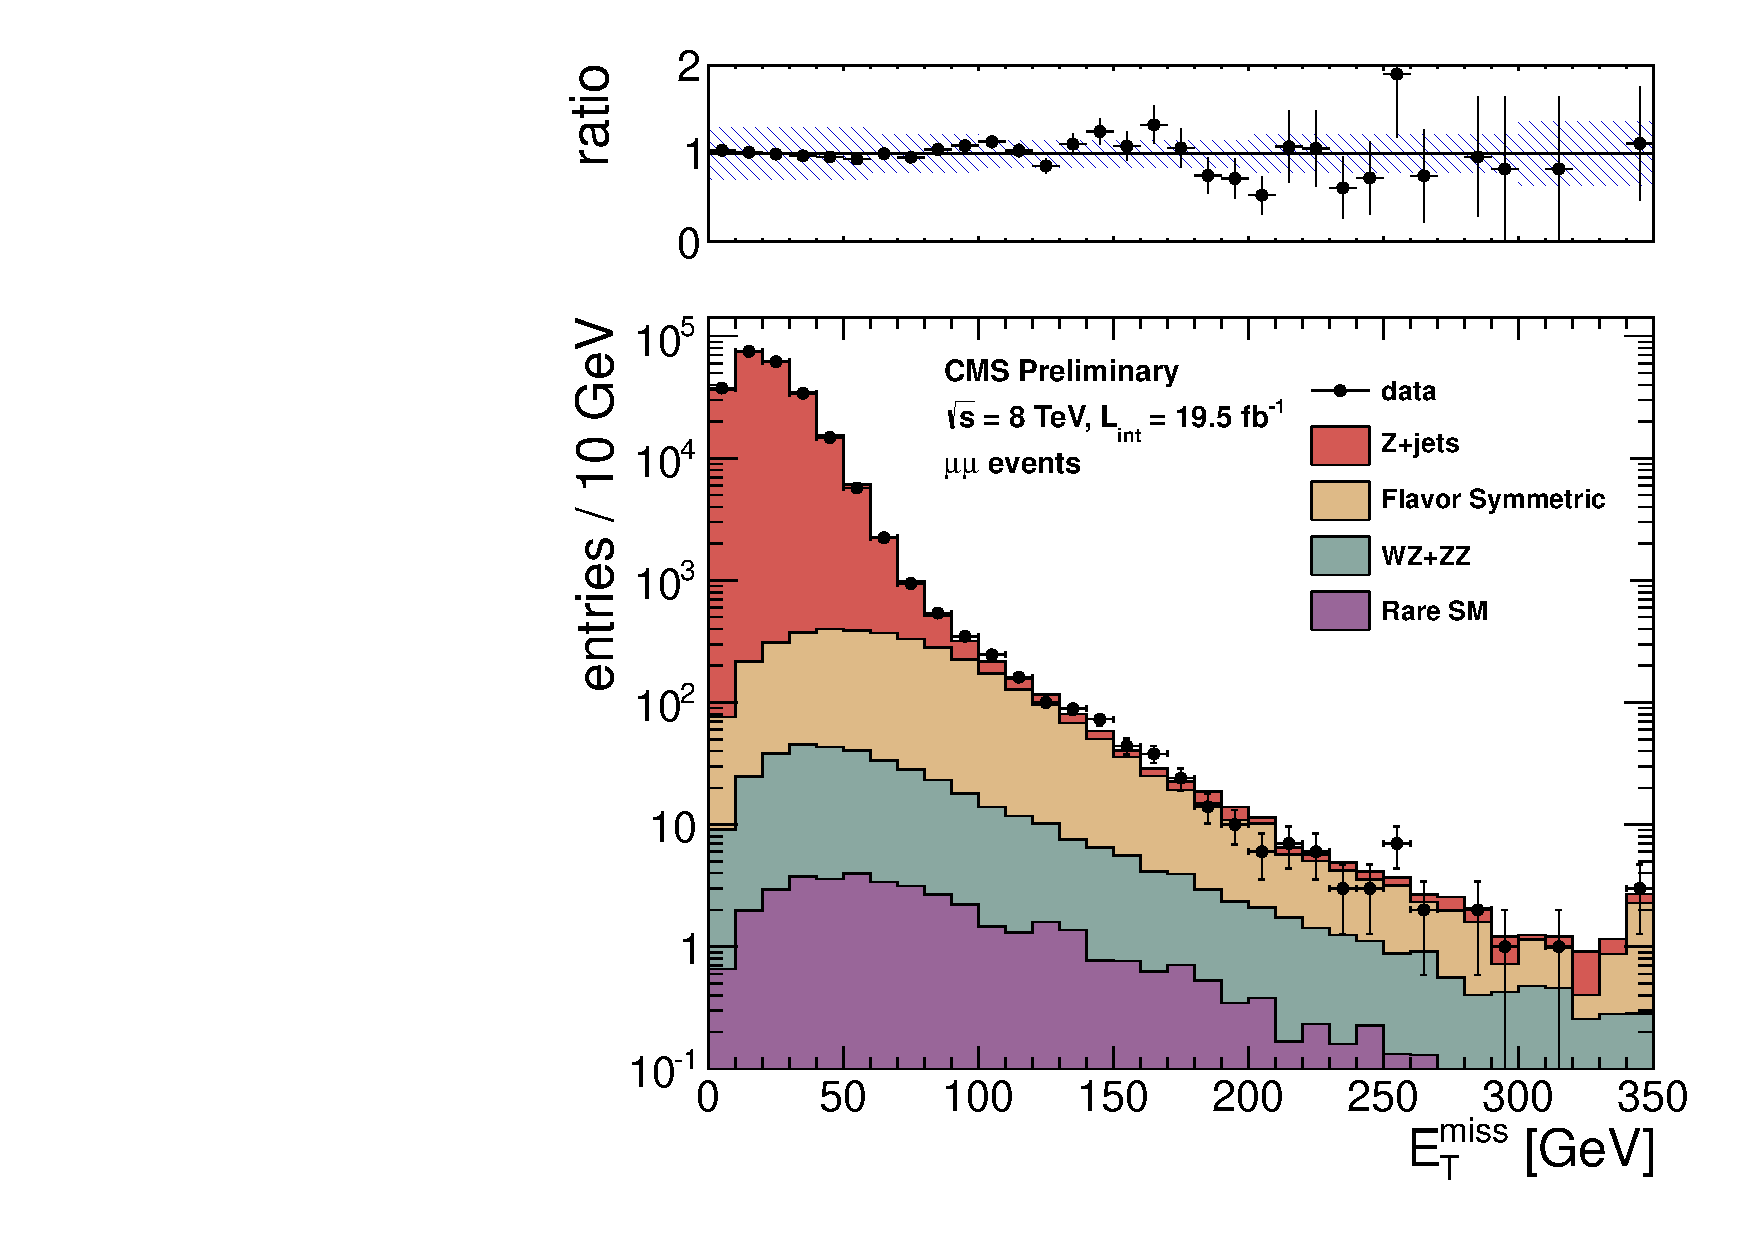
\includegraphics[width=0.6\textwidth]{plots/pfmet_mm_19p5fb.pdf}
\end{tabular}
\caption{Results of the inclusive analysis in the $\mu\mu$ channel. The observed \MET\ distribution (black points) is compared with the sum of the predicted \MET\
distributions from \zjets, flavor-symmetric backgrounds, and WZ+ZZ backgrounds. The ratio of observed to predicted yields in each bin is
indicated. The error bars indicate the statistical uncertainty in the data and the shaded band indicates the total background uncertainty.
\label{fig:results_incl_mm}
}
\end{center}
\end{figure}

\begin{table}[htb]
\begin{center}
\footnotesize
\caption{\label{tab:results_incl_mm} Summary of results in the inclusive analysis in the $\mu\mu$ channel. The total background is the sum of the \zjets\ background predicted from
the \MET\ templates method (\zjets\ bkg), the flavor-symmetric background predicted from e$\mu$ events (FS bkg), and the WZ and ZZ backgrounds predicted from MC
(WZ bkg and ZZ bkg). All uncertainties include both the statistical and systematic components. The Gaussian significance of the deviation between the data 
and total background is indicated for signal regions with at least 20 observed events. }
\begin{tabular}{l|c|c|c|c|c|c}

\hline
\hline

%mm channel: scale em yield by 0.53
%Yields in 0-60 GeV region
%data   : 229222
%gjets  : 231217
%OF     : 1563.54
%WZ     : 162.693
%ZZ     : 21.5319
%Rare   : 16.8552
%Scaling gjets by : 0.983741
%SF events 234132
%OF events 43832

%#mu#mu events

                      &   \MET\ 0--30 GeV   &  \MET\ 30--60 GeV   & \MET\ 60--100 GeV   &\MET\ 100--200 GeV   &\MET\ 200--300 GeV   & \MET\ $>$ 300 GeV  \\
\hline
        \zjets\ bkg   &172758 $\pm$ 51829   & 54699 $\pm$ 16412   &    2752 $\pm$ 828   &      122 $\pm$ 44   &     6.2 $\pm$ 1.9   &     1.4 $\pm$ 0.5  \\
             FS bkg   &      531 $\pm$ 99   &    1032 $\pm$ 193   &    1105 $\pm$ 206   &     553 $\pm$ 103   &    27.7 $\pm$ 8.7   &     3.9 $\pm$ 2.4  \\
             WZ bkg   &   59.9 $\pm$ 30.0   &  102.8 $\pm$ 51.4   &   75.1 $\pm$ 37.6   &   43.0 $\pm$ 21.5   &     5.9 $\pm$ 3.0   &     1.6 $\pm$ 1.6  \\
             ZZ bkg   &     6.8 $\pm$ 3.4   &    14.7 $\pm$ 7.4   &    16.6 $\pm$ 8.3   &    16.5 $\pm$ 8.3   &     3.3 $\pm$ 1.6   &     1.1 $\pm$ 1.1  \\
        rare SM bkg   &     5.6 $\pm$ 2.8   &    11.3 $\pm$ 5.7   &    11.4 $\pm$ 5.7   &     9.5 $\pm$ 4.8   &     1.6 $\pm$ 0.8   &     0.6 $\pm$ 0.6  \\
\hline
          total bkg   &173362 $\pm$ 51829   & 55860 $\pm$ 16413   &    3959 $\pm$ 854   &     744 $\pm$ 115   &    44.6 $\pm$ 9.6   &     8.7 $\pm$ 3.2  \\
               data   &            174626   &             54596   &              4070   &               799   &                37   &                 4  \\
%       significance   &       0.0$\sigma$   &      -0.1$\sigma$   &       0.1$\sigma$   &       0.5$\sigma$   &      -0.7$\sigma$   &      -1.2$\sigma$  \\
\hline
\hline


%float Zbkg_yield[nbins]    = { 122.0 ,  6.2 ,     1.4  };
%float Zbkg_err[nbins]      = { 44.2 ,  1.9 ,     0.5  };
%float OFbkg_yield[nbins]   = { 552.6 , 27.7 ,     3.9  };
%float OFbkg_err[nbins]     = { 103.3 ,  8.7 ,     2.4  };
%float WZbkg_yield[nbins]   = { 43.0 ,  5.9 ,     1.6  };
%float WZbkg_err[nbins]     = { 21.5 ,  3.0 ,     1.6  };
%float ZZbkg_yield[nbins]   = { 16.5 ,  3.3 ,     1.1  };
%float ZZbkg_err[nbins]     = {  8.3 ,  1.6 ,     1.1  };
%float rarebkg_yield[nbins] = {  9.5 ,  1.6 ,     0.6  };
%float rarebkg_err[nbins]   = {  4.8 ,  0.8 ,     0.6  };
%int   data_yield[nbins]    = {  799 ,   37 ,       4  };


\end{tabular}
\end{center}
\end{table}


\clearpage

The \MET\ distributions in the targeted analysis for the ee channel are displayed in Fig.~\ref{fig:results_targ_ee} and 
the signal region yields are presented in Table~\ref{tab:results_targ_ee}.
The \MET\ distributions in the inclusive analysis for the $\mu\mu$ channel are displayed in Fig.~\ref{fig:results_targ_mm} and 
the signal region yields are presented in Table~\ref{tab:results_targ_mm}.

\begin{figure}[!h]
\begin{center}
\begin{tabular}{cc}
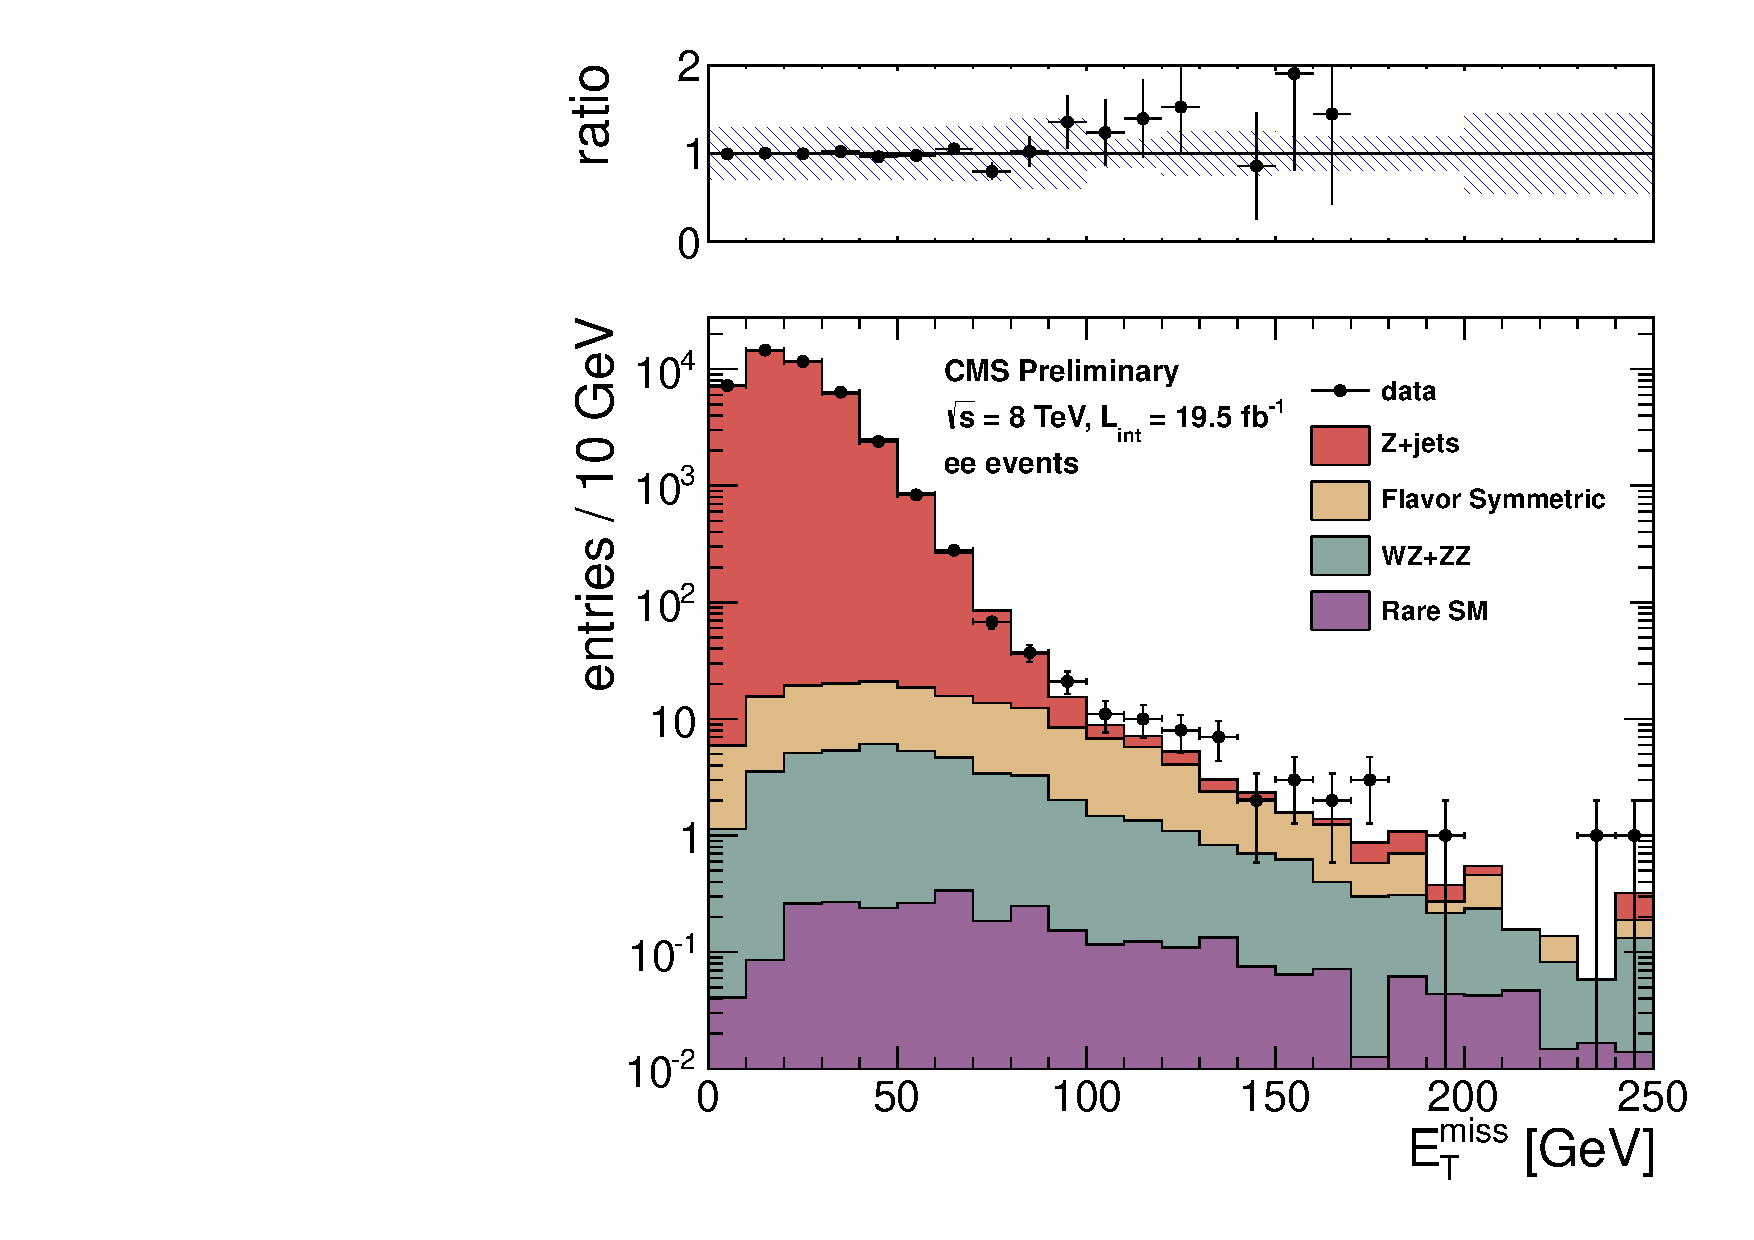
\includegraphics[width=0.5\textwidth]{plots/pfmet_bveto_ee_19p5fb.pdf}
\end{tabular}
\caption{Results of the targeted analysis in the ee channel. The observed \MET\ distribution (black points) is compared with the sum of the predicted \MET\
distributions from \zjets, flavor-symmetric backgrounds, and WZ+ZZ backgrounds. The ratio of observed to predicted yields in each bin is
indicated. The error bars indicate the statistical uncertainty in the data and the shaded band indicates the total background uncertainty.
\label{fig:results_targ_ee}
}
\end{center}
\end{figure}



\begin{table}[htb]
\begin{center}
\footnotesize
\caption{\label{tab:results_targ_ee}\footnotesize Summary of results in the targeted analysis in the ee channel. The total background is the sum of the \zjets\ background predicted from
the \MET\ templates method (\zjets\ bkg), the flavor-symmetric background predicted from e$\mu$ events (FS bkg), and the WZ and ZZ backgrounds predicted from MC
(WZ bkg and ZZ bkg). All uncertainties include both the statistical and systematic components. The Gaussian significance of the deviation between the data 
and total background is indicated for signal regions with at least 20 observed events. }
\begin{tabular}{l|c|c|c|c}

%ee channel: scale em yield by 0.43
%Yields in 0-60 GeV region
%data   : 42990
%gjets  : 43100.4
%OF     : 73.8439
%WZ     : 19.284
%ZZ     : 3.91603
%Rare   : 0.668177
%Scaling gjets by : 0.995172
%SF events 43444
%OF events 2313

%ee events

\hline
\hline
                      &   \MET\ 0--30 GeV   &  \MET\ 30--60 GeV   &  \MET\ 60--80 GeV   & \MET\ 80--100 GeV    \\
\hline
\hline
        \zjets\ bkg   &  33491 $\pm$ 1344   &    9401 $\pm$ 380   &      307 $\pm$ 68   &    28.8 $\pm$ 9.9    \\
             FS bkg   &    31.0 $\pm$ 6.2   &    42.9 $\pm$ 8.5   &    21.4 $\pm$ 4.3   &    15.6 $\pm$ 3.2    \\
             WZ bkg   &     7.3 $\pm$ 3.7   &    12.0 $\pm$ 6.0   &     5.5 $\pm$ 2.8   &     3.3 $\pm$ 1.7    \\
             ZZ bkg   &     1.3 $\pm$ 0.7   &     2.6 $\pm$ 1.3   &     1.5 $\pm$ 0.7   &     1.3 $\pm$ 0.6    \\
        Rare SM bkg   &     0.2 $\pm$ 0.1   &     0.4 $\pm$ 0.2   &     0.3 $\pm$ 0.1   &     0.2 $\pm$ 0.1    \\
\hline
          Total bkg   &  33531 $\pm$ 1344   &    9459 $\pm$ 380   &      335 $\pm$ 68   &   49.2 $\pm$ 10.5    \\
               Data   &             33420   &              9570   &               347   &                58    \\
      %significance   &      -0.1$\sigma$   &       0.3$\sigma$   &       0.2$\sigma$   &       0.7$\sigma$    \\
\hline
\hline
                      &\MET\ 100--120 GeV   &\MET\ 120--150 GeV   &\MET\ 150--200 GeV   & \MET\ $>$ 200 GeV  \\
\hline
\hline
        \zjets\ bkg   &     3.5 $\pm$ 1.4   &     1.6 $\pm$ 0.7   &     0.9 $\pm$ 0.4   &     0.2 $\pm$ 0.2  \\
             FS bkg   &     9.7 $\pm$ 2.0   &     5.9 $\pm$ 1.3   &     2.5 $\pm$ 0.8   &     0.3 $\pm$ 0.2  \\
             WZ bkg   &     1.6 $\pm$ 0.8   &     1.4 $\pm$ 0.7   &     0.8 $\pm$ 0.4   &     0.3 $\pm$ 0.2  \\
             ZZ bkg   &     0.7 $\pm$ 0.4   &     0.7 $\pm$ 0.4   &     0.7 $\pm$ 0.4   &     0.6 $\pm$ 0.3  \\
        Rare SM bkg   &     0.1 $\pm$ 0.1   &     0.1 $\pm$ 0.1   &     0.2 $\pm$ 0.1   &     0.1 $\pm$ 0.1  \\
\hline
          Total bkg   &    15.6 $\pm$ 2.6   &     9.6 $\pm$ 1.7   &     5.1 $\pm$ 1.0   &     1.6 $\pm$ 0.5  \\
               Data   &                21   &                17   &                 9   &                 2  \\
      %significance   &       1.0$\sigma$   &       1.7$\sigma$   &       1.2$\sigma$   &       0.2$\sigma$  \\
\hline
\hline



\end{tabular}
\end{center}
\end{table}


\clearpage

\begin{figure}[!h]
\begin{center}
\begin{tabular}{cc}
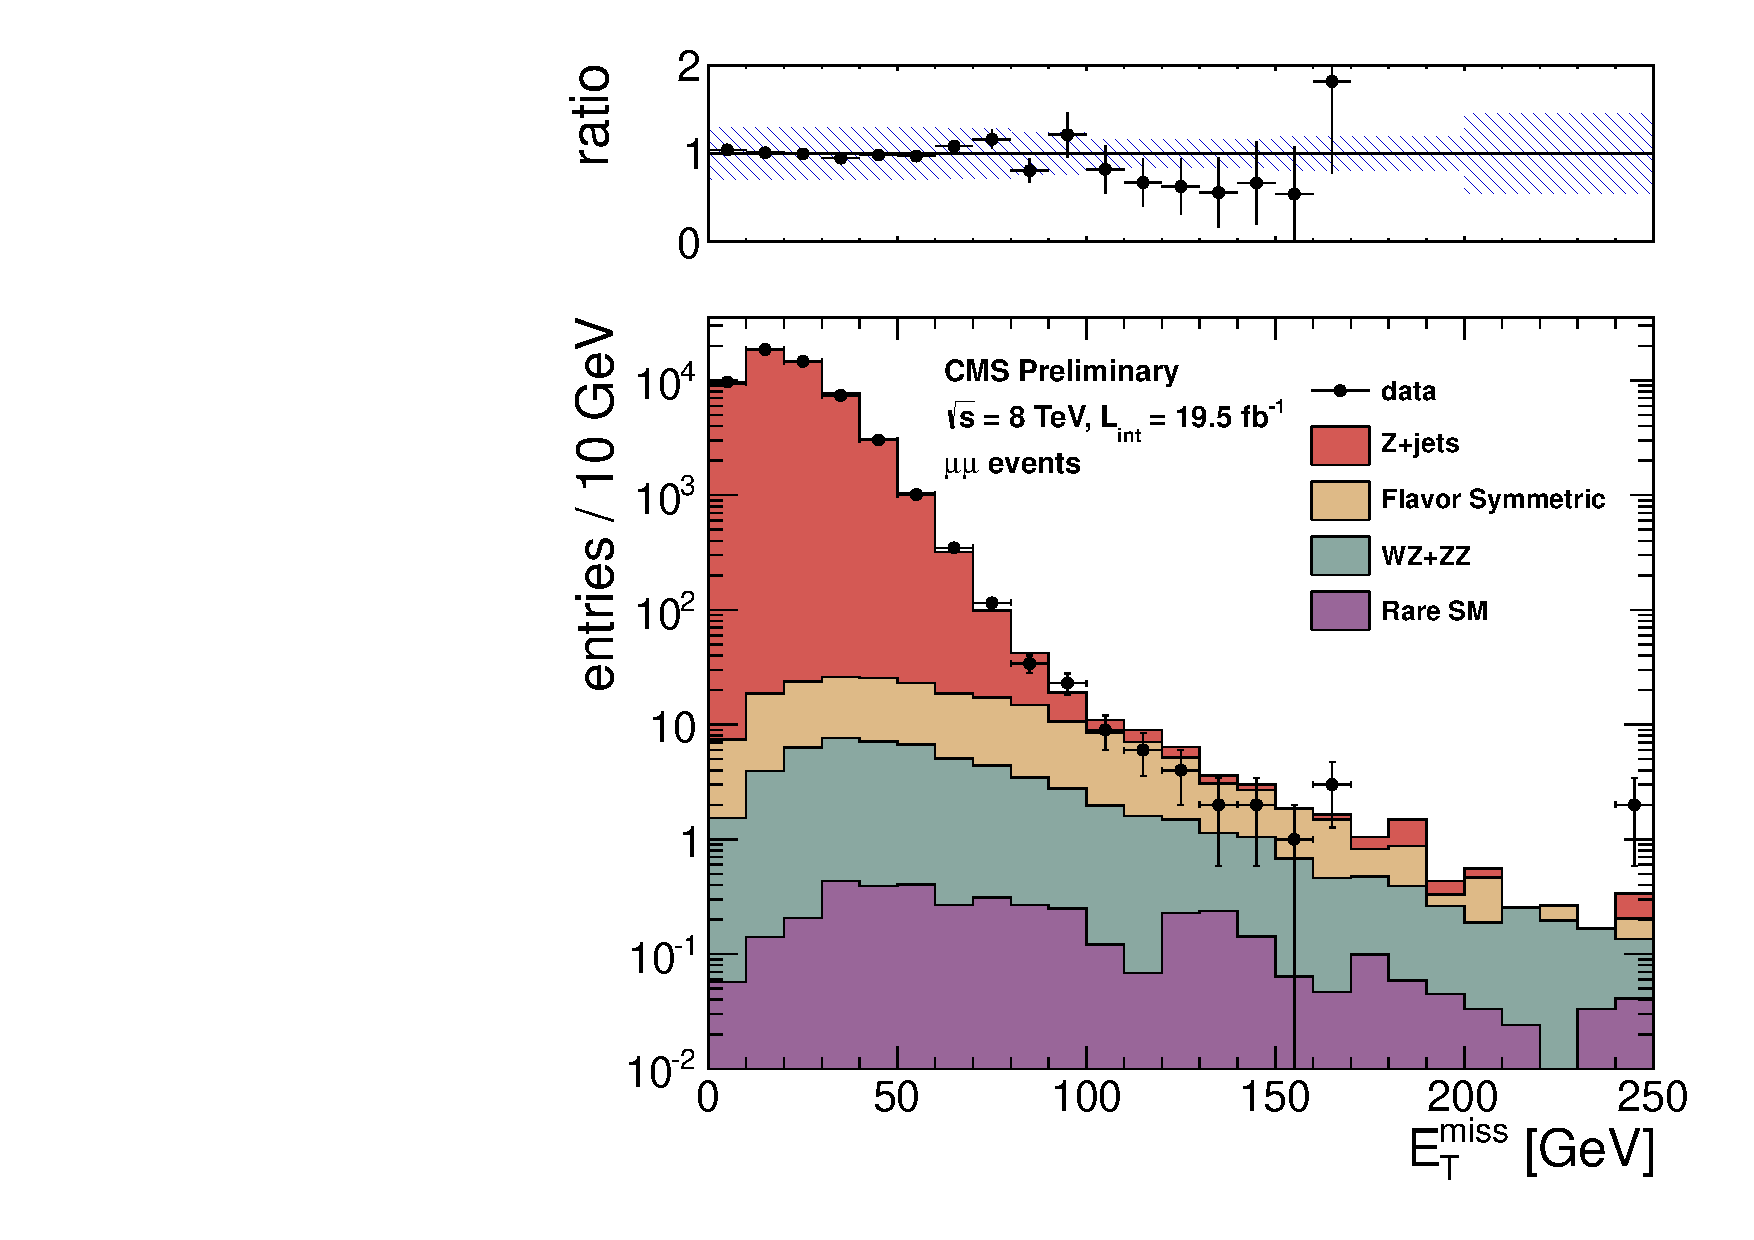
\includegraphics[width=0.5\textwidth]{plots/pfmet_bveto_mm_19p5fb.pdf}
\end{tabular}
\caption{Results of the targeted analysis in the $\mu\mu$ channel. The observed \MET\ distribution (black points) is compared with the sum of the predicted \MET\
distributions from \zjets, flavor-symmetric backgrounds, and WZ+ZZ backgrounds. The ratio of observed to predicted yields in each bin is
indicated. The error bars indicate the statistical uncertainty in the data and the shaded band indicates the total background uncertainty.
\label{fig:results_targ_mm}
}
\end{center}
\end{figure}



\begin{table}[htb]
\begin{center}
\footnotesize
\caption{\label{tab:results_targ_mm}\footnotesize Summary of results in the targeted analysis in the $\mu\mu$ channel. The total background is the sum of 
the \zjets\ background predicted from
the \MET\ templates method (\zjets\ bkg), the flavor-symmetric background predicted from e$\mu$ events (FS bkg), and the WZ and ZZ backgrounds predicted from MC
(WZ bkg and ZZ bkg). All uncertainties include both the statistical and systematic components. The Gaussian significance of the deviation between the data 
and total background is indicated for signal regions with at least 20 observed events. }
\begin{tabular}{l|c|c|c|c}

%mm channel: scale em yield by 0.53
%Yields in 0-60 GeV region
%data   : 54303
%gjets  : 54422
%OF     : 91.0169
%WZ     : 23.941
%ZZ     : 4.90294
%Rare   : 0.790992
%Scaling gjets by : 0.995597
%SF events 54851
%OF events 2313

%#mu#mu events

\hline
\hline
                      &\MET\ 100--120 GeV   &\MET\ 120--150 GeV   &\MET\ 150--200 GeV   & \MET\ $>$ 200 GeV  \\
\hline
\hline
        \zjets\ bkg   &     4.3 $\pm$ 1.7   &     2.1 $\pm$ 0.9   &     1.1 $\pm$ 0.5   &     0.2 $\pm$ 0.2  \\
             FS bkg   &    12.0 $\pm$ 2.5   &     7.2 $\pm$ 1.6   &     3.1 $\pm$ 0.9   &     0.4 $\pm$ 0.2  \\
             WZ bkg   &     2.1 $\pm$ 1.1   &     1.6 $\pm$ 0.8   &     1.0 $\pm$ 0.5   &     0.5 $\pm$ 0.3  \\
             ZZ bkg   &     1.0 $\pm$ 0.5   &     1.2 $\pm$ 0.6   &     0.8 $\pm$ 0.4   &     0.7 $\pm$ 0.3  \\
        Rare SM bkg   &     0.1 $\pm$ 0.0   &     0.3 $\pm$ 0.2   &     0.2 $\pm$ 0.1   &     0.1 $\pm$ 0.1  \\
\hline
          Total bkg   &    19.6 $\pm$ 3.3   &    12.4 $\pm$ 2.1   &     6.2 $\pm$ 1.3   &     1.9 $\pm$ 0.5  \\
               Data   &                15   &                 8   &                 4   &                 2  \\
      %significance   &      -0.9$\sigma$   &      -1.2$\sigma$   &      -0.9$\sigma$   &       0.0$\sigma$  \\
\hline
\hline

                      &\MET\ 100--120 GeV   &\MET\ 120--150 GeV   &\MET\ 150--200 GeV   & \MET\ $>$ 200 GeV  \\
\hline
\hline
        \zjets\ bkg   &     4.3 $\pm$ 1.7   &     2.1 $\pm$ 0.9   &     1.1 $\pm$ 0.5   &     0.2 $\pm$ 0.2  \\
             FS bkg   &    12.0 $\pm$ 2.5   &     7.2 $\pm$ 1.6   &     3.1 $\pm$ 0.9   &     0.4 $\pm$ 0.2  \\
             WZ bkg   &     2.1 $\pm$ 1.1   &     1.6 $\pm$ 0.8   &     1.0 $\pm$ 0.5   &     0.5 $\pm$ 0.3  \\
             ZZ bkg   &     1.0 $\pm$ 0.5   &     1.2 $\pm$ 0.6   &     0.8 $\pm$ 0.4   &     0.7 $\pm$ 0.3  \\
        Rare SM bkg   &     0.1 $\pm$ 0.0   &     0.3 $\pm$ 0.2   &     0.2 $\pm$ 0.1   &     0.1 $\pm$ 0.1  \\
\hline
          Total bkg   &    19.6 $\pm$ 3.3   &    12.4 $\pm$ 2.1   &     6.2 $\pm$ 1.3   &     1.9 $\pm$ 0.5  \\
               Data   &                15   &                 8   &                 4   &                 2  \\
      %significance   &      -0.9$\sigma$   &      -1.2$\sigma$   &      -0.9$\sigma$   &       0.0$\sigma$  \\
\hline
\hline


\end{tabular}
\end{center}
\end{table}


%\input{appendix_WZ.tex}
\clearpage
\section{MET Templates from Photon Sample}
\label{sec:appendix_templates}

In this appendix we display our templates derived from the photon sample 
using the HLTPhoton20 (Fig.~\ref{fig:template20}), HLTPhoton30 (Fig.~\ref{fig:template30}),
HLTPhoton50 (Fig.~\ref{fig:template50}) and HLTPhoton70 (Fig.~\ref{fig:template70}) triggers.


\begin{figure}[hbt]
  \begin{center}
    \resizebox{0.7\linewidth}{!}{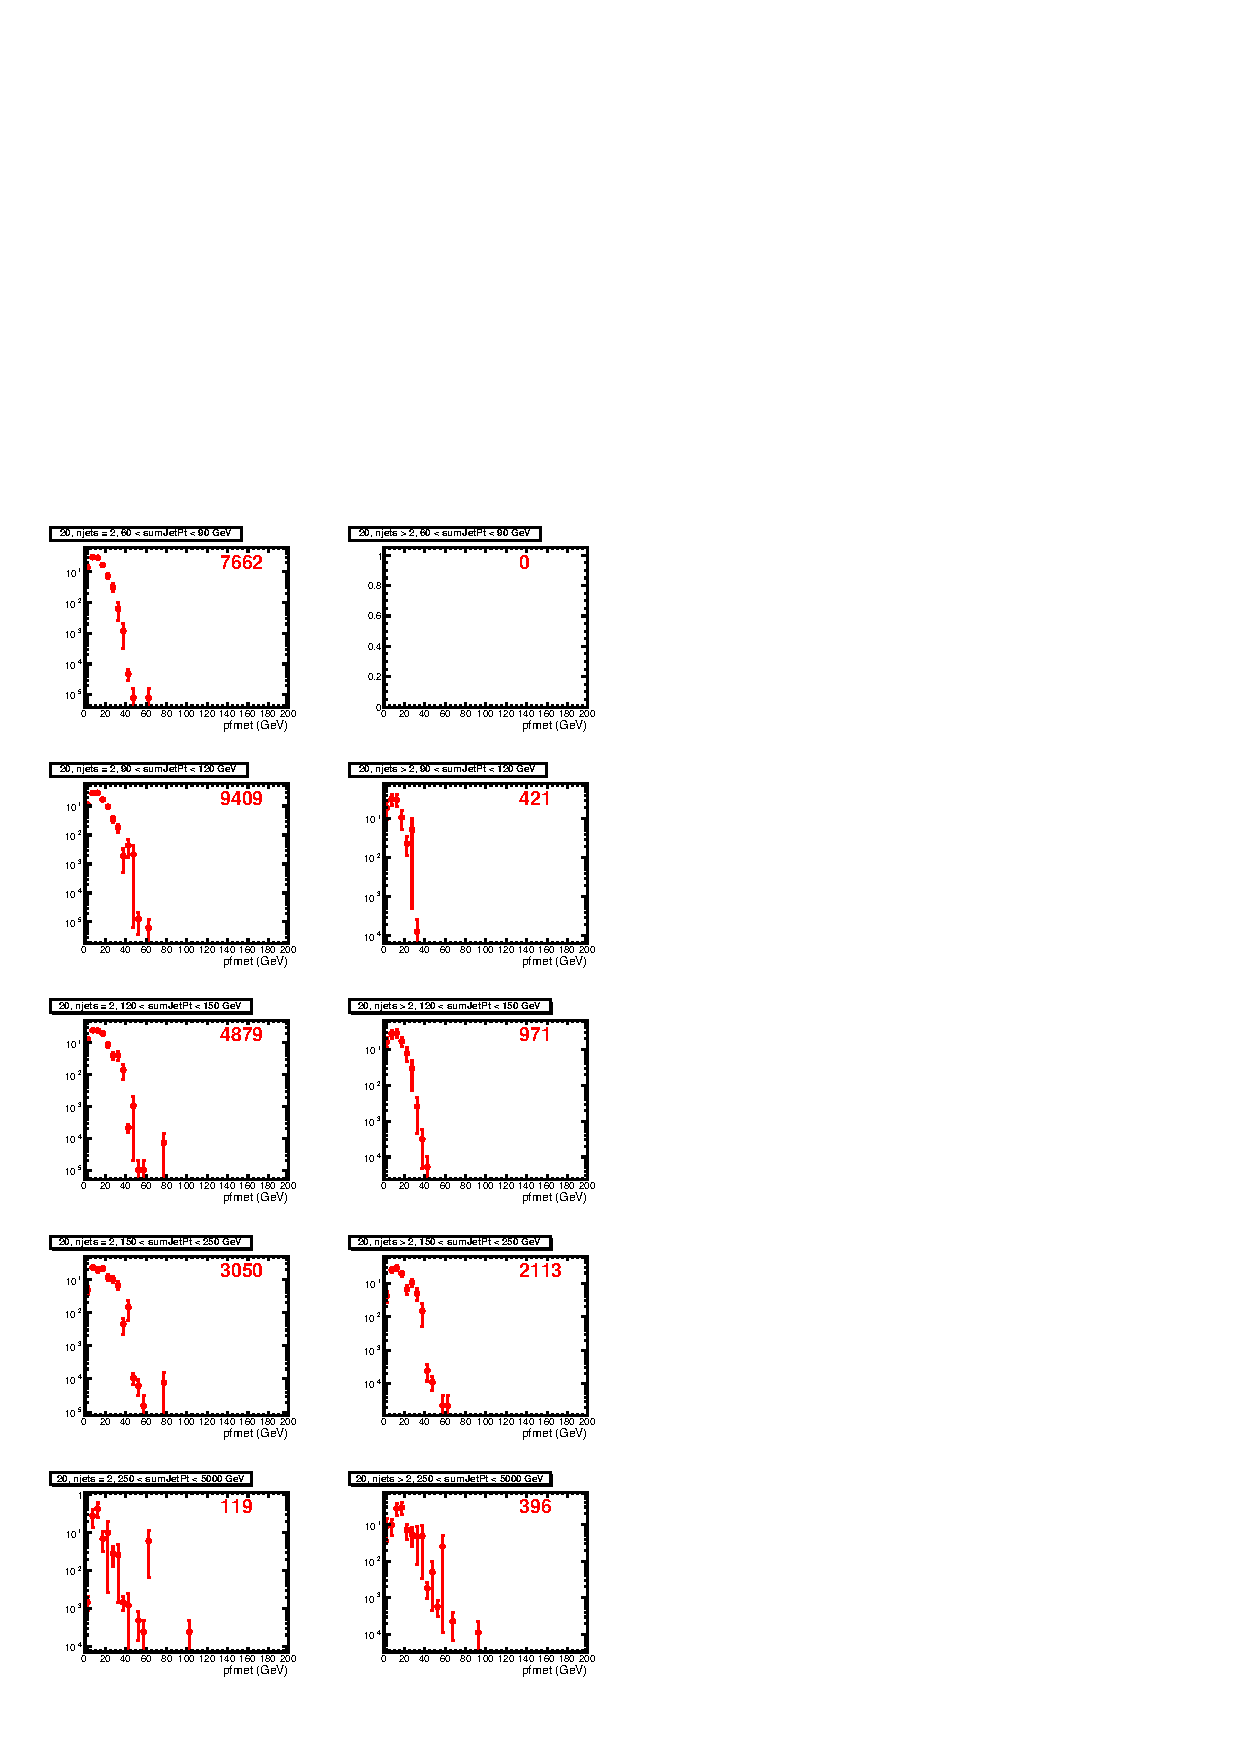
\includegraphics{plots/template_20.pdf}}
    \caption{MET Templates derived from the HLTPhoton20 sample.}
    \label{fig:template20}
  \end{center}
\end{figure}

\begin{figure}[hbt]
  \begin{center}
    \resizebox{0.7\linewidth}{!}{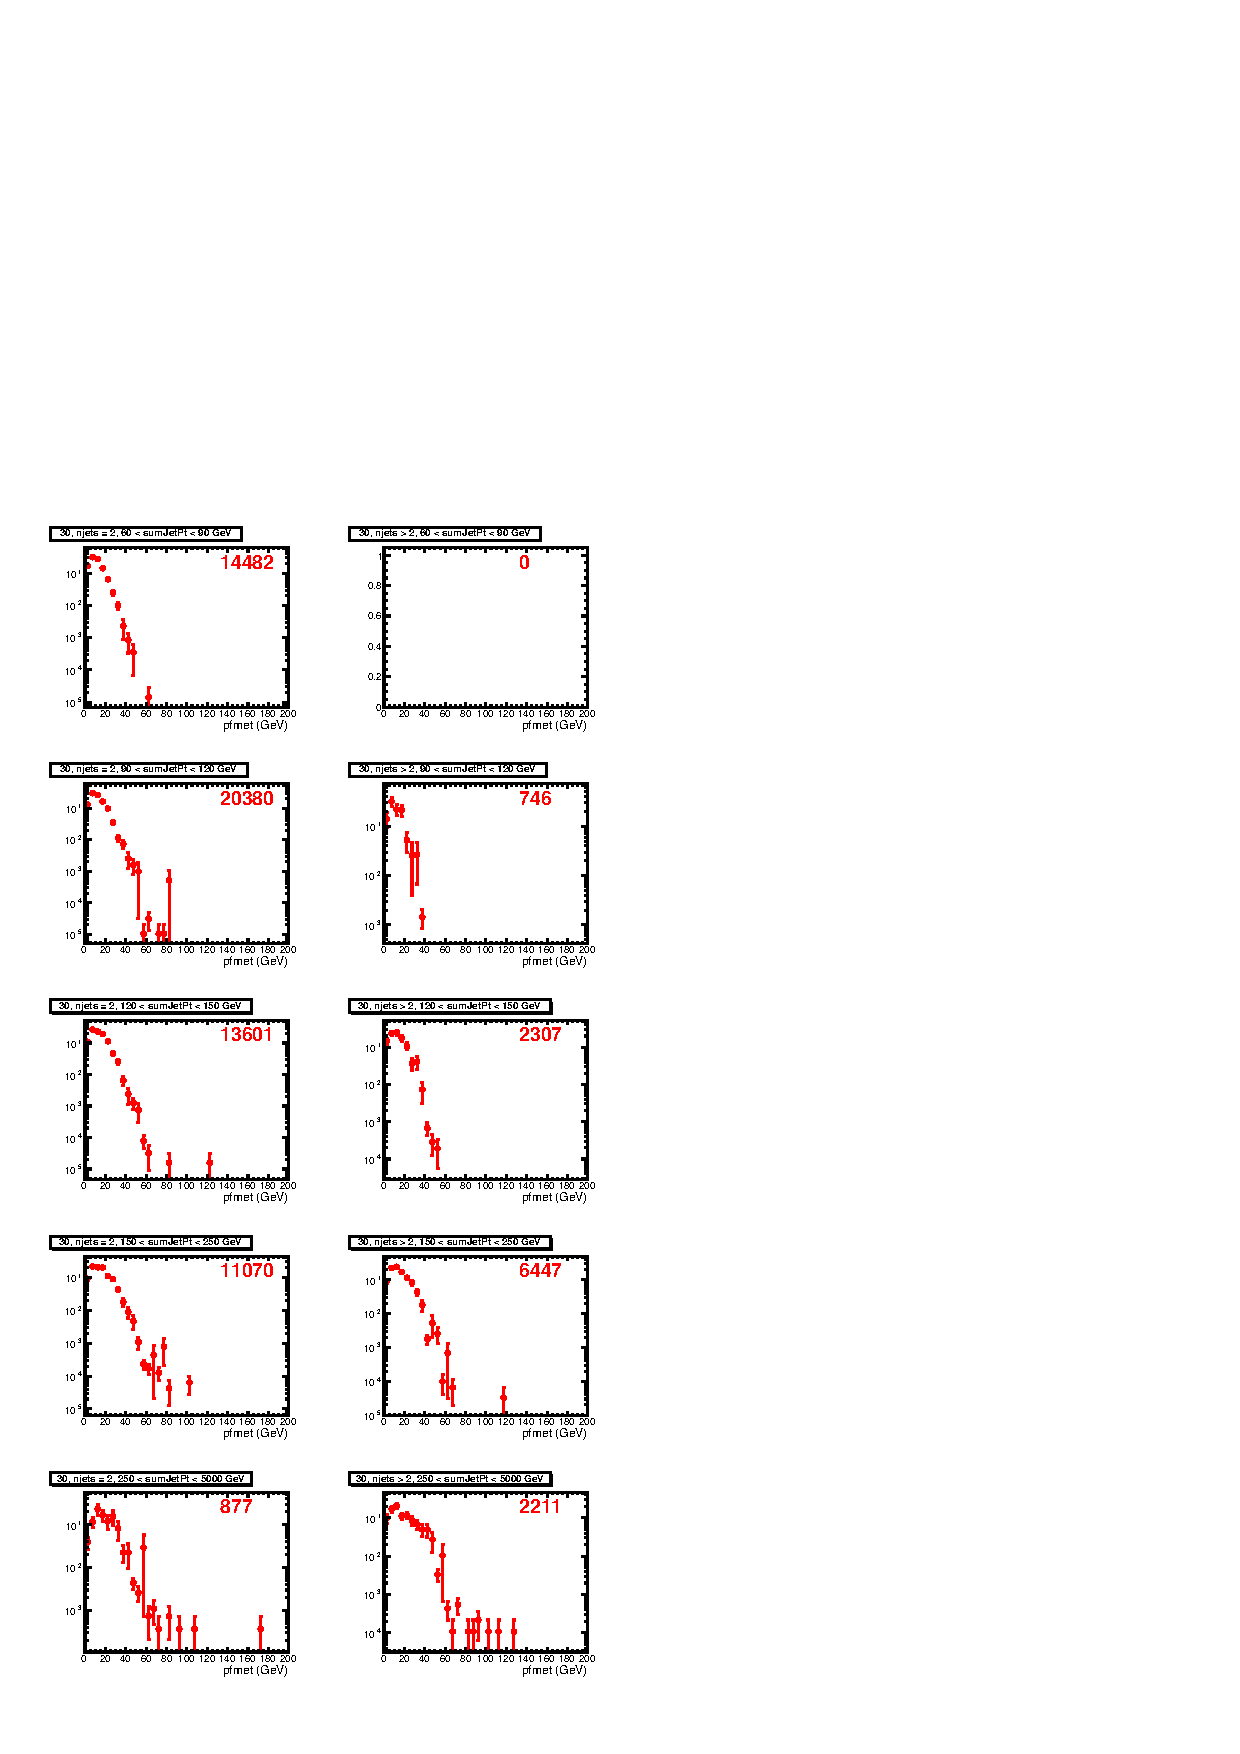
\includegraphics{plots/template_30.pdf}}
    \caption{MET Templates derived from the HLTPhoton30 sample.}
    \label{fig:template30}
  \end{center}
\end{figure}

\begin{figure}[hbt]
  \begin{center}
    \resizebox{0.7\linewidth}{!}{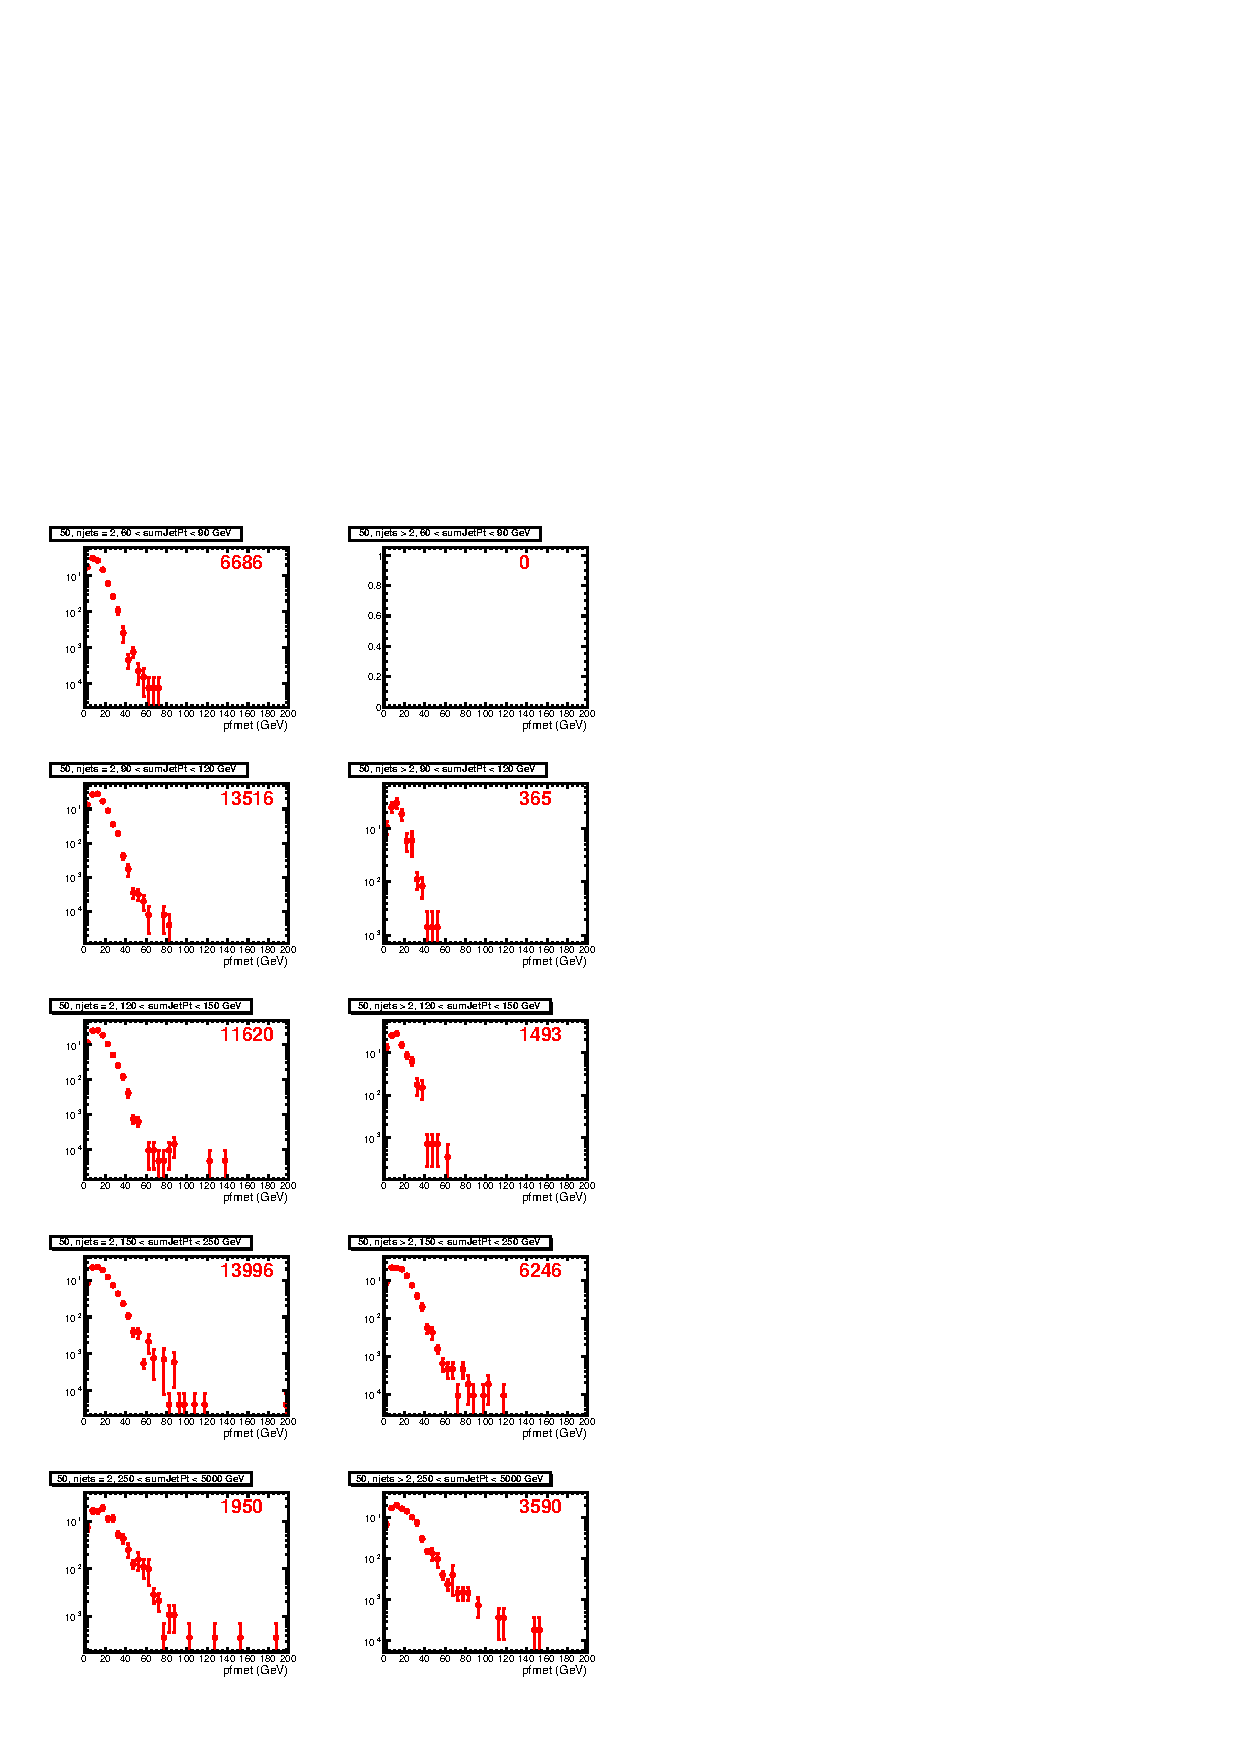
\includegraphics{plots/template_50.pdf}}
    \caption{MET Templates derived from the HLTPhoton50 sample.}
    \label{fig:template50}
  \end{center}
\end{figure}

\begin{figure}[hbt]
  \begin{center}
    \resizebox{0.7\linewidth}{!}{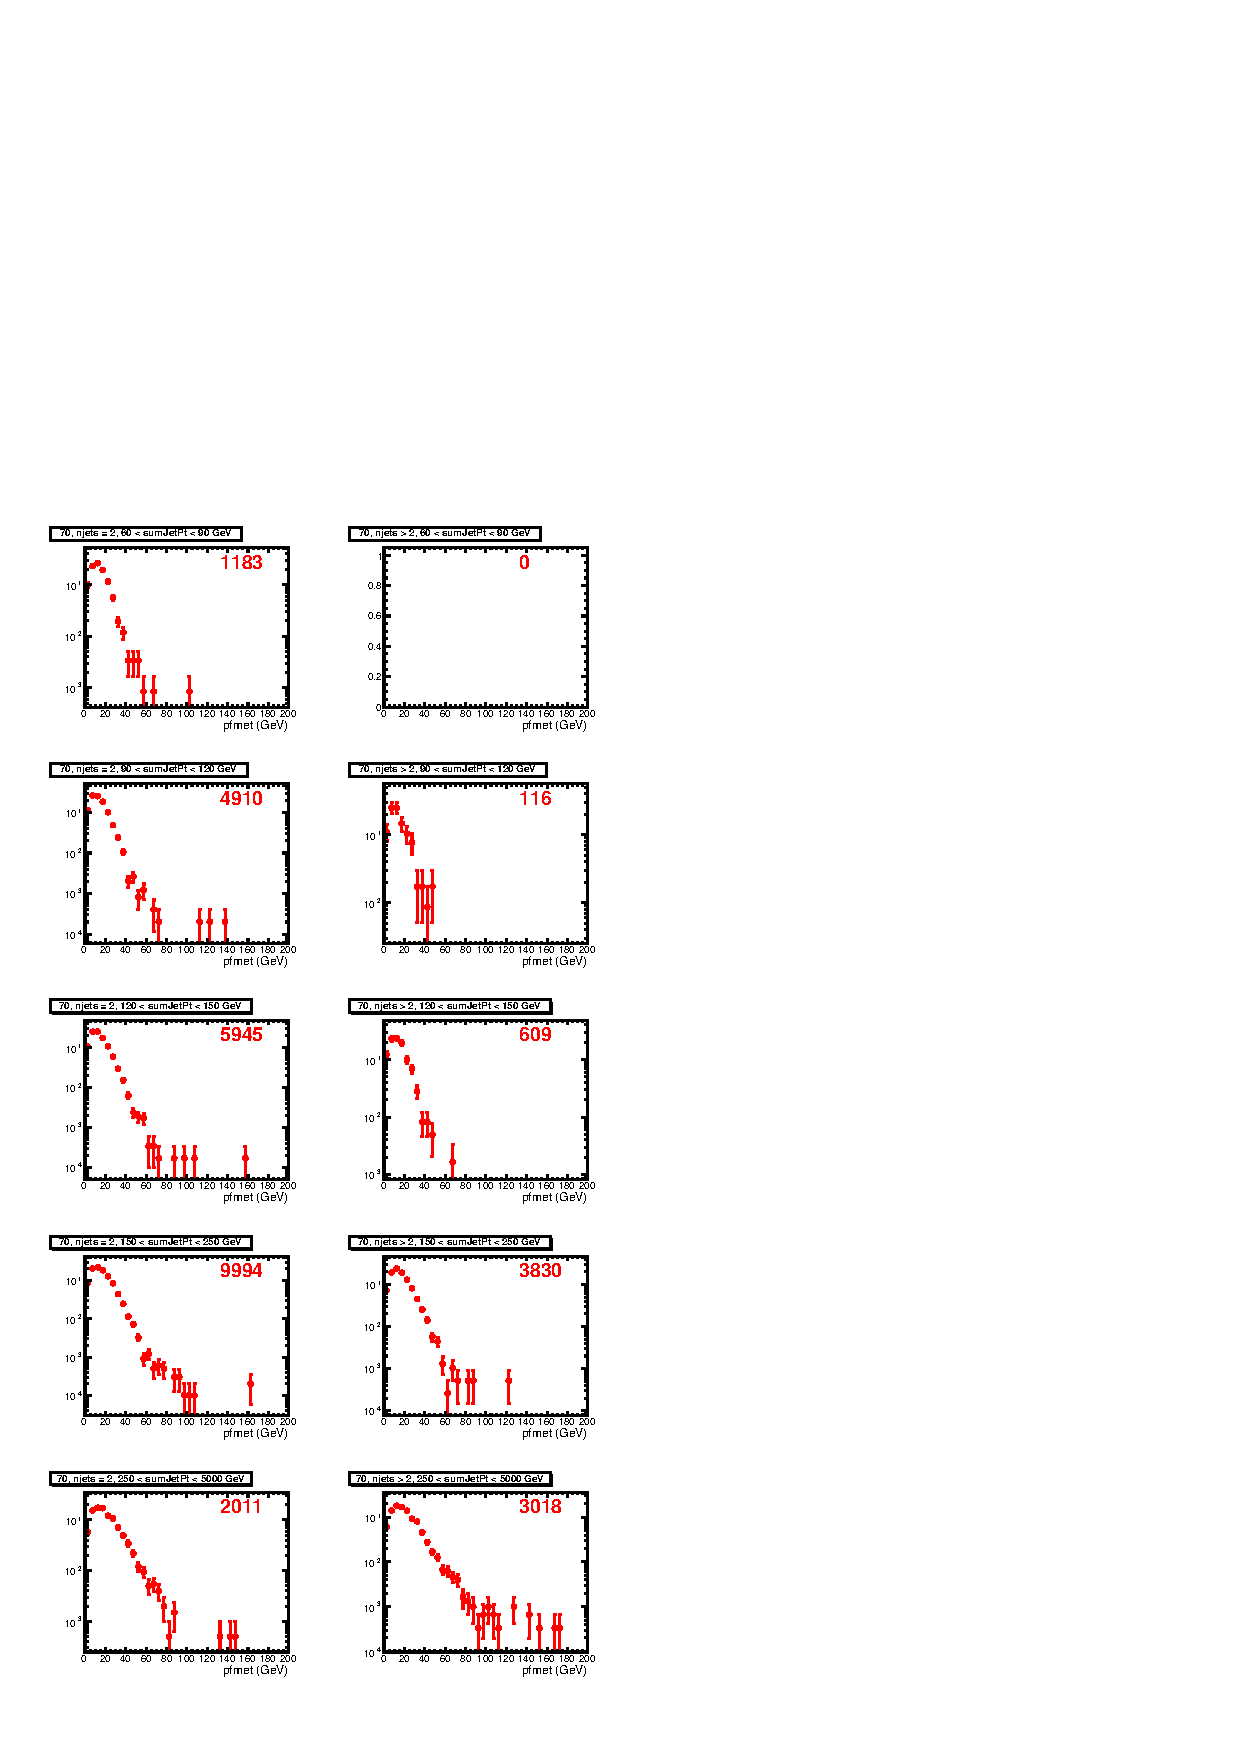
\includegraphics{plots/template_70.pdf}}
    \caption{MET Templates derived from the HLTPhoton70 sample.}
    \label{fig:template70}
  \end{center}
\end{figure}



\end{document}
